\chapter{Experiments}
\label{chap:experiments}

\section{Empirical performance testing}

This section presents the methodology and results of the empirical performance testing of the selected algorithms on the selected benchmarks, using the framework which was designed and implemented for this thesis.
The goal of this phase is to design and run experiments to evaluate the performance of the algorithms on the benchmarks, and based on the empirical results, which are backup-up by statistical tests, formulate
hypotheses on the relative performance of the algorithms given the problem class, and suggest guidelines for the choice of algorithms, as well as for the choice of parameters for these algorithms.

In the following sections, results are presented for each algorithm on the selected benchmark problems they can be applied to, in chronological order of the experiments.
This allows for a detailed analysis of the performance of each of the algorithms and experimentation with various configurations, before comparing them on the same problems, as well as
motivating the different experiments which were conducted. Then, following the comparison, guidelines for the choice of algorithms and parameters are formulated..

\subsection{Methodology}

As it is the case with the literature review, it is important to define a clear and systematic methodology for the empirical performance testing phase. This will ensure the reproducibility of the experiments,
and the validity of the results.

First of all, it is worth noting that the implementation of the different algorithms and benchmarks as parts of a ingle framework, is a key factor in ensuring the fairness of the comparison between the different
algorithms and the validity of the results. Indeed, the different algorithms are implemented in the same language, are queried using a same API, and are run on the same hardware. However, this also means that
errors or small changes in the implementation of the algorithms or benchmarks are possible, and could thus affect the results compared to the original descriptions or implementations.

As one of the goal of the experiments is to evaluate different configurations of the algorithms, the ideal experiment would consist in testing all possible parameters of the algorithms on all possible benchmarks.
However, this is obviously not feasible, as there are infinitely many possible configurations of the algorithms. Therefore, the experiments will be designed to test a subset of the possible configurations, which
will be chosen based on intuition and the literature review. Furthermore, since guidelines for the choice of parameters are sought, experiments will be guided towards
better performance of the algorithms on the problems. This is done by iteratively identifying the parameter values which lead to better performance, and testing more configurations around these values, in order
to refine the choice of parameters.

\subsubsection{Performance measures}

The goal of the experiments is to evaluate the performance of algorithms on benchmark problems, but how is performance defined in this case? The performance of an algorithm can be measured in many way,
depending on the problem and goals. For example, in the case of a sorting algorithm, performance could be measured as the number of comparisons, but in a context where memory usage is important, it is also
worth considering the space complexity of the algorithm.

In the case of this thesis, the following performance measures are considered:

\begin{itemize}
    \item \textbf{Execution time}: the time taken by the algorithm to solve the problem.
    \item \textbf{Quality of the solution}: the quality of the solution found by the algorithm, i.e the fitness of the best performing individual in the final population. For the implemented benchmarks, all
    fitness values are in the range $[0, 1]$, and the higher the fitness, the better the solution.
    \item \textbf{Generations}: the number of generations taken by the algorithm to solve the problem. This metrics only makes sens because of the "early stopping" criterion used in the implementation of the
    algorithms, which stops the algorithm when a fitness threshold is reached.
\end{itemize}

\subsubsection{Testing workflows in practice}

Given the high computational cost induced by the high number of experiments to run, the experiments were run on the high-performance computing cluster (HPC) of DTU.
This will make it possible to benefit from the high number of cores available in the cluster, because of the parallel nature of the implemented testing logic.
More precisely, the central DTU HPC cluster (LSF 10) was used \footnote{\url{https://www.hpc.dtu.dk/?page_id=2520}}.
It contains nodes with 10, 12, 16 or 24 cores. Applications are run on the cluster by mean of job scripts, with the resource manager
parsing the scripts and handling the usage of the available resources. Job scripts contain speciation for the resources requirements, job constraints, a specific queue to use and commands to setup the environment
and run the application. Queues are used to order jobs which are not run immediately.

In addition to running the unit-tests, by having the target set to linux, it also allows to verify that the project should be able to compile on the HPC.
An example of a job script is shown in Listing \ref{lst:job_script}, it runs the $(1 + 1)$ NA algorithm on the \textit{Quarter} benchmark with a resolution of 50 to 1000, and 1000 runs
for each resolution, and saves the results in CSV files. The configuration of the job script is done using the LSF directives, which are comments starting with \texttt{\#BSUB}.

\begin{lstlisting}[language=bash, caption=Example of a job script, label=lst:job_script]
#!/bin/sh

#### General options
### -- specify queue --
#BSUB -q hpc
### -- set the job Name --
#BSUB -J Bench
### -- ask for number of cores (default: 1) --
#BSUB -n 10
### -- specify that the cores must be on the same host --
#BSUB -R "span[hosts=1]"
### -- specify that we need 4GB of memory per core/slot --
#BSUB -R "rusage[mem=4GB]"
### -- specify that we want the job to get killed if it exceeds 5 GB per core/slot --
#BSUB -M 5GB
### -- set walltime limit: hh:mm --
#BSUB -W 24:00
### -- set the email address --
# please uncomment the following line and put in your e-mail address,
# if you want to receive e-mail notifications on a non-default address
#BSUB -u s222887@dtu.dk
### -- send notification at start --
#BSUB -B
### -- send notification at completion --
#BSUB -N
### -- Specify the output and error file. %J is the job-id --
### -- -o and -e mean append, -oo and -eo mean overwrite --
#BSUB -o ~/Output_%J.out
#BSUB -e ~/Output_%J.err

n_runs=1000
problem=quarter
algorithm=oneplusonena

cd ~/code-master

for resolution in $(seq 50 50 1500)
do
    ./target/release/main $algorithm $problem -i 200 -n 1 \\
    -r $resolution -t $n_runs \\
    -o ~/output/$algorithm/$problem/$algorithm_$problem_$resolution.csv
done
\end{lstlisting}

A python script was written to merge the results of the different runs in a single CPU file, extract the relevant metrics and statistics, and output data which directly be used
in the \textt{pgfplots} plots of this report.

\section{Results of the experiments}
\label{sec:results}

This section presents the results of the different experiments which were conducted to highlight properties of the algorithms, observe the impact of different parameters on the performance,
and evaluate the algorithms on the selected benchmarks.

\subsection{Results of the $(1 + 1)$ NA algorithm}

The $(1 + 1)$ NA algorithm can be applied to binary classification problems. Results are thus presented for the unit-sphere classification problems, the \textit{XOR} problem, and
the \texit{Cancer1} classification problem.
The parameters which can be tuned for this algorithm are the resolution and the number of neurons.

\subsubsection{Unit-sphere classification problems}

The unit-sphere classification problems \cite{na} were introduced to evaluate the $(1 + 1)$ NA algorithm. For these simple problems, optimal solutions are known. In particular, these
problems can be used to observe some of the properties of the algorithm.

The first experiment consisted in running the algorithm with different configurations on the simple \texttt{Half} and \texttt{Quarter} benchmarks.
Results for these benchmarks are shown in \Cref{fig:na_maxiter}. The maximum number of iteration was set to $200$, and the evolution stopped when the fitness
was $2\%$ away from the maximal fitness of $1.0$. Since these tasks can be solved with a single neuron, the number of neurons was set to $1$ and different resolutions ranging
from $2$ to $1500$ were tested. The results show that, for small resolutions, the algorithm is unable to solve the problems, and thus stops after $200$ iterations. This is
because such low resolutions do not allow to set the parameters to values which are close enough to the optimal ones. On the other hand,
for resolutions allowing for a finer discretization of the space, the algorithm is always able to find the optimal solutions, and the number of iteration it takes to do so
does not vary with the resolution over the tested range. Lastly, these results also show, that as expected, the CPU time is proportional to the number of iterations,
as the same steps are performed by the algorithm at each generation.

Because of the lack of a stagnation criteria in the previous experiment, the algorithm would only stop when it reached a fitness close enough to the optimal on, or when
the maximum number of iterations was reached. As it can be seen with the results for the lower resolutions, this is far from ideal, as the algorithm continues to run even
though no progress can be made.

\Cref{fig:na_half_stagnation} and \Cref{fig:na_quarter_stagnation} show the results of the $(1 + 1)$ NA algorithm on the \textit{Half} and \textit{Quarter} benchmarks, with a single neuron, over
resolutions ranging from $2$ to $1500$, but with different values of maximum stagnation iterations. The maximum number of iterations was kept at $200$, and the evolution stopped when the fitness
was $2\%$ away from the maximal fitness of $1.0$. Five different values of maximum stagnation iterations were tested, ranging from only $5$ generations to $80$ generations, which is close to
the number of iterations it takes solve the problems, as it can be seen in \Cref{fig:na_maxiter}.

This time, the algorithm is not always solving the problem, even for high-enough resolutions. Higher number of stagnant iterations allow the algorithm to reach a higher fitness, but at the
expanse of more iterations (and thus, more CPU time). As a matter of fact, for the \textit{Half} problem and a resolution of $800$, the algorithm reaches, on average, a fitness of
$0.84$ and stops after $15$ iterations with $5$ stagnant iterations, while it reaches a fitness of $0.98$ after $69$ iterations with $80$ stagnant iterations.
In addition, this stagnation criteria allows to stop the algorithm for the small resolutions of $2$ and $5$, while still letting the algorithm reach the maximal possible fitnesses in these
two cases. Lastly, an interesting phenomenon can be observed on both problems, for stagnant iterations values of $60$ and $80$ arond resolutions of a $100$, where the number of iterations
is at its highest. This can also be observed in the results of the previous experiment, when ignoring the lower resolutions, and could be explained by these resolutions being hgh enough
to allow for setting the parameters to set the parameters to values which are close enough to the optimal ones, but not high enough to make drawing these values as liely as for higher resolutions.
% TODO check and detail

The more complex \textit{TwoQuarters} problem requires two neurons to be solved. With a single neuron, the best fitness that can be achieved is $0.75$, because at least a quarter of the unit sphere
cannot be classified correctly with a single decision line. Such a solution is shown in \Cref{fig:na_twoquarters_single_visual}.
\Cref{fig:na_twoquarters} shows the results of the $(1 + 1)$ NA algorithm on the \textit{TwoQuarters} benchmark, with a single or two neurons,
a fixed resolution of $400$, and values of maximum iterations ranging from $50$ to $2500$. The evolution stopped when the fitness was $2\%$ away from the maximal fitness of $1.0$ or
the maximum number of iterations was reached. The resolution of $400$ was chosen based on the results of the previous experiments, where it could be seen that this value was in the range of
resolutions where the problems could be solved and the number of iterations needed to do so was the lowest and not varying.

\begin{figure}
    \centering
    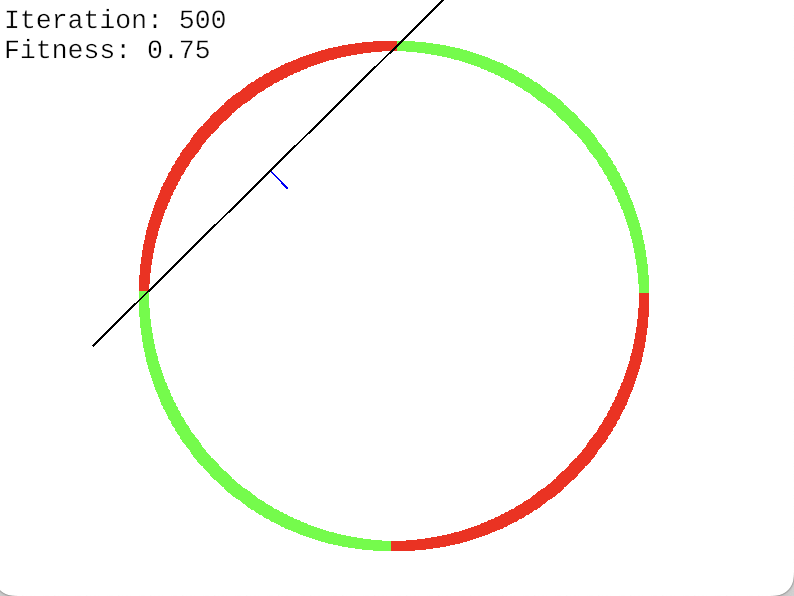
\includegraphics[width=7cm]{Pictures/twoquarters-single}
    \caption{Visualization of a solution with a fitness of $0.75$ after evolution of the $(1 + 1)$ NA algorithm with one neuron on the \textit{TwoQuarters} problem.
    The top-left quarter of the unit sphere is misclassified.}
    \label{fig:na_twoquarters_single_visual}
\end{figure}

As expected, in the case of one neuron, the algorithm is unable to solve the problem, and the maximum fitness of $0.75$ is almost reached at the lowest tested maximum number of iterations of $50$.
As a consequence, it can also be seen that the number of iterations taken by the algorithm is equal to the maximum number of iterations, since the fitness is never within $2\%$ of the optimal one.
In the case of two neurons, the algorithm, which can theoretically solve the problem, achieves a higher average fitness, but is unable to find the optimal solutions on all runs and gets stuck
at a local optima with a fitness of $0.75$. The optimal solution and an example of a local optima are shown in \Cref{fig:na_twoquarters_visual}.
It can be seen that the number of iterations taken by the algorithm in the case of two neurons is lower than for one neuron. However, the CPU time is higher, because of iterations being more
computationally expensive, as the algorithm has to evolve two neurons instead of one.
Furthermore, the average fitness, iterations and CPU time all seem to grow logarithmically with the maximum number of iterations.

\begin{figure}
    \centering
    \begin{subfigure}{0.45\textwidth}
        \centering
        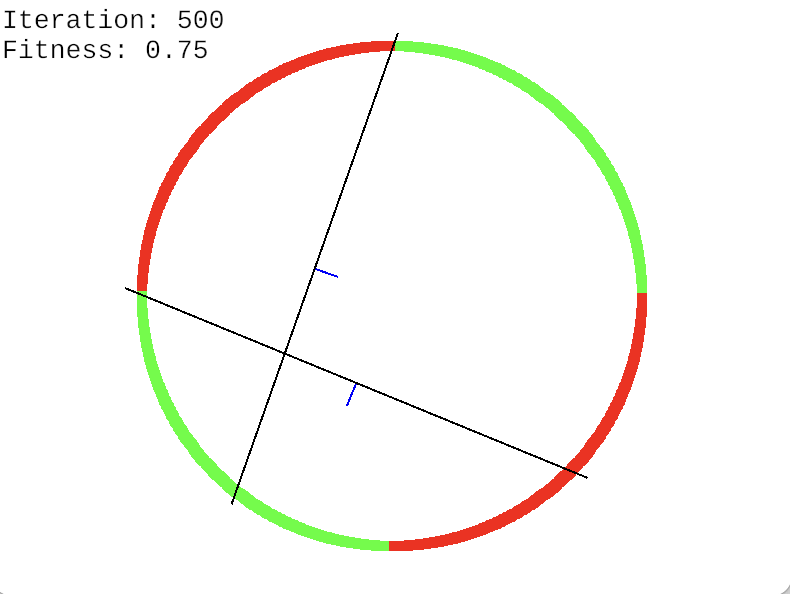
\includegraphics[width=0.9\textwidth]{Pictures/twoquarters-localopt}
       \caption{Local optima}
    \end{subfigure}\hfill
    \begin{subfigure}{0.45\textwidth}
        \centering
        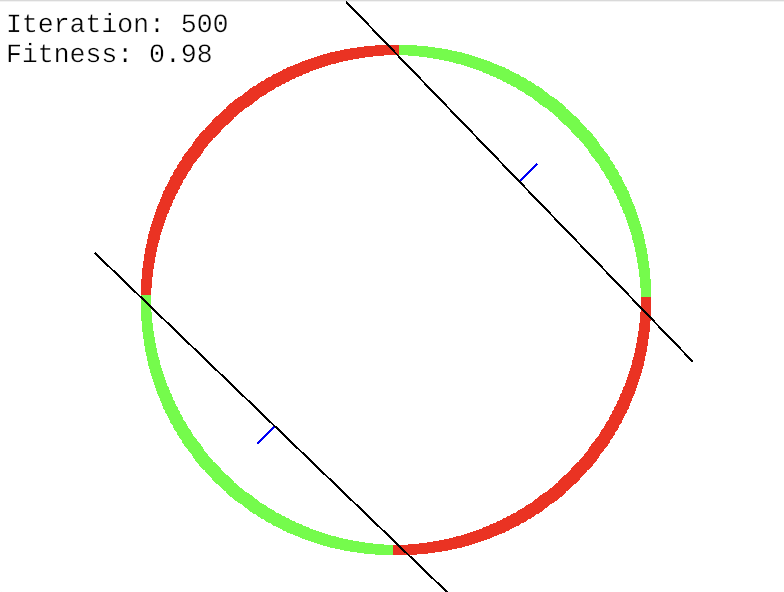
\includegraphics[width=0.9\textwidth]{Pictures/twoquarters-opt}
        \caption{Optimal solution}
    \end{subfigure}
    \caption{Visualization of two configurations of the $(1 + 1)$ NA algorithm, with two neurons, after evolution on the \textit{TwoQuarters} problem.}
    \label{fig:na_twoquarters_visual}
\end{figure}

In \Cref{fig:na_twoquarters_stag}, the results of the algorithm, with two neurons, on the \textit{TwoQuarters} problem are shown with different values of maximum stagnation iterations. The other
parameters were kept the same as in the previous experiment, and the number of stagnant iterations was varied from $5$ to $1000$ with a step size of $20$. On average, the algorithm stops before $1200$
iterations, without always solving the task, even when it is allowed to stagnate for $1000$ iterations. This shows how hard it is for the algorithm to leave the local optima it gets stuck in.

Finally, the \textit{LocalOpt} problem requires three neurons to be solved. For this problem, there are local optima with fitnesses of $0.75$ and $0.9$, as shown in \Cref{fig:na_localopt_visual}.
\Cref{fig:na_localopt} shows the results of the algorithm on this problem, with a fixed resolution of $400$, one, two or three neurons, and maximum number of iterations ranging from $50$ to $2000$.
The evolution stopped when the fitness was $2\%$ away from the maximal fitness of $1.0$ or the maximum number of iterations was reached. For all configurations, the algorithm was unable to solve
the problem. In the case of one neuron, it reaches the maximum possible fitness of $0.75$ after approximately $200$ iterations. The fitness curve for two and three neurons are almost identical,
and converge to a fitness of $0.85$. Since the algorithm was unable to find the optimal solution, the maximum number of iterations was always reached, while the CPU time results reflect the
impact of the number of neurons on the computational cost of the algorithm.

\begin{figure}
    \centering
    \begin{subfigure}{0.45\textwidth}
        \centering
        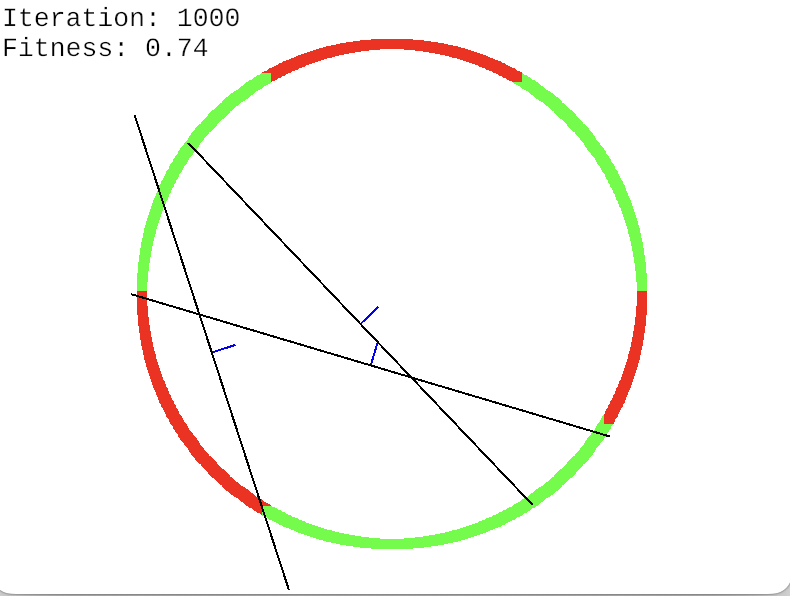
\includegraphics[width=0.9\textwidth]{Pictures/localopt_75}
       \caption{Local optima with fitness of $0.75$}
    \end{subfigure}\hfill
    \begin{subfigure}{0.45\textwidth}
        \centering
        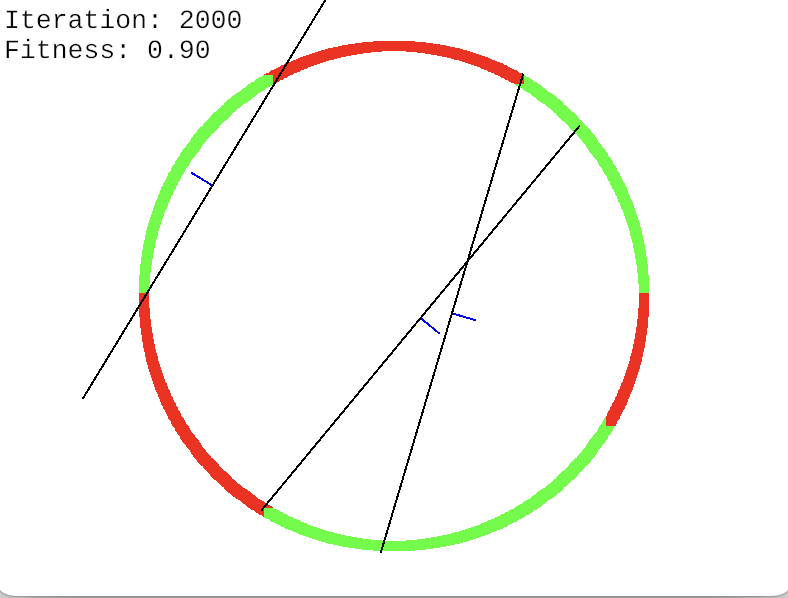
\includegraphics[width=0.9\textwidth]{Pictures/localopt_90}
        \caption{Local optima with fitness of $0.9$}
    \end{subfigure}
    \caption{Visualization of two configurations of the $(1 + 1)$ NA algorithm, with three neurons, after evolution on the \textit{LocalOpt} problem.}
    \label{fig:na_localopt_visual}
\end{figure}

% TODO discuss how initialization is more important, greedy nature, lack of exploration, cpu time vs number of neurons, more iterations are for fine-tuning, not linearly separable but one neuron is best etc.

\begin{figure}
    \begin{center}
        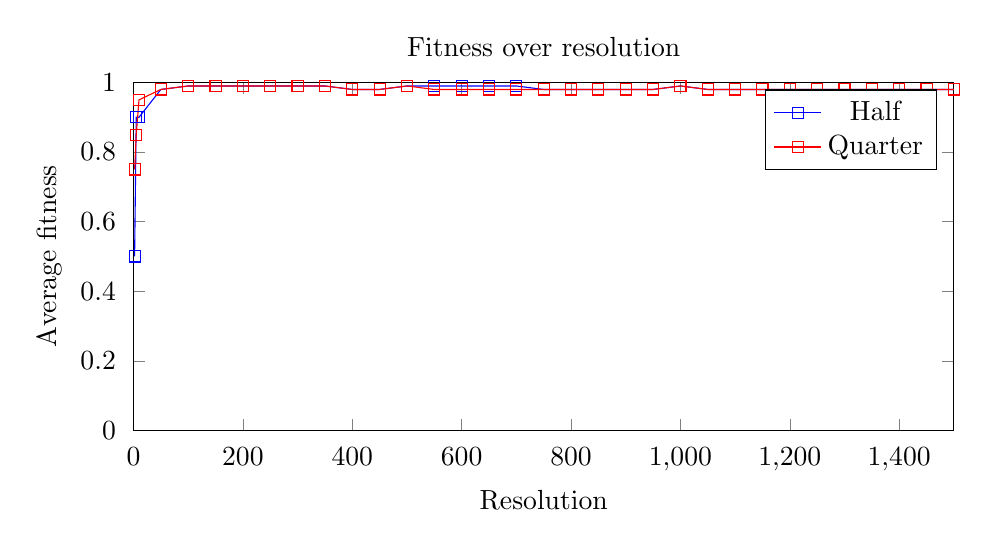
\begin{tikzpicture}
        \begin{axis}[
            width=12cm,
            height=6cm,
            title={Fitness over resolution},
            xlabel={Resolution},
            ylabel={Average fitness},
            enlargelimits=false,
            xmin=0,
            ymin=0, ymax=1,
            ytick={0,0.2,...,1},
            xticklabel shift={.1cm},
            yticklabel shift={.1cm} ]
        ]

        \addplot[
            color=blue,
            mark=square,
            ]
            coordinates {
                (2,0.50)(5,0.90)(10,0.90)(50,0.98)(100,0.99)(150,0.99)(200,0.99)(250,0.99)(300,0.99)(350,0.99)(400,0.98)(450,0.98)(500,0.99)(550,0.99)(600,0.99)(650,0.99)(700,0.99)(750,0.98)(800,0.98)(850,0.98)(900,0.98)(950,0.98)(1000,0.99)(1050,0.98)(1100,0.98)(1150,0.98)(1200,0.98)(1250,0.98)(1300,0.98)(1350,0.98)(1400,0.98)(1450,0.98)(1500,0.98)
            };
            \addlegendentry{Half}
        \addplot[
            color=red,
            mark=square,
            ]
            coordinates {
                (2,0.75)(5,0.85)(10,0.95)(50,0.98)(100,0.99)(150,0.99)(200,0.99)(250,0.99)(300,0.99)(350,0.99)(400,0.98)(450,0.98)(500,0.99)(550,0.98)(600,0.98)(650,0.98)(700,0.98)(750,0.98)(800,0.98)(850,0.98)(900,0.98)(950,0.98)(1000,0.99)(1050,0.98)(1100,0.98)(1150,0.98)(1200,0.98)(1250,0.98)(1300,0.98)(1350,0.98)(1400,0.98)(1450,0.98)(1500,0.98)
            };
            \addlegendentry{Quarter}
        \end{axis}
        \end{tikzpicture}
        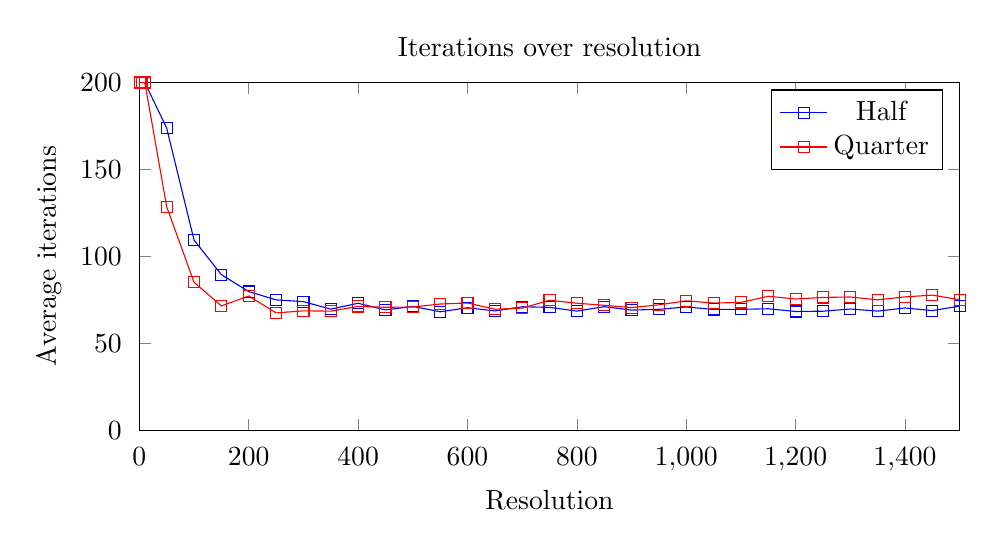
\begin{tikzpicture}
        \begin{axis}[
            width=12cm,
            height=6cm,
            title={Iterations over resolution},
            xlabel={Resolution},
            ylabel={Average iterations},
            xmin=0,
            ymin=0,
            enlargelimits=false,
            xticklabel shift={.1cm},
            yticklabel shift={.1cm} ]
        ]

        \addplot[
            color=blue,
            mark=square,
            ]
            coordinates {
                (2,200.00)(5,200.00)(10,200.00)(50,173.75)(100,109.39)(150,89.55)(200,79.81)(250,75.03)(300,74.03)(350,69.72)(400,73.08)(450,69.26)(500,71.27)(550,68.19)(600,70.51)(650,68.69)(700,71.07)(750,70.74)(800,68.57)(850,71.13)(900,69.16)(950,69.63)(1000,70.95)(1050,69.54)(1100,69.62)(1150,69.92)(1200,68.36)(1250,68.52)(1300,69.78)(1350,68.57)(1400,70.38)(1450,68.86)(1500,71.47)
            };
            \addlegendentry{Half}
        \addplot[
            color=red,
            mark=square,
            ]
            coordinates {
                (2,200.00)(5,200.00)(10,200.00)(50,128.58)(100,85.14)(150,71.56)(200,77.29)(250,67.54)(300,68.72)(350,68.57)(400,71.26)(450,70.78)(500,70.92)(550,72.64)(600,73.26)(650,69.66)(700,70.31)(750,74.80)(800,73.12)(850,71.89)(900,70.59)(950,72.19)(1000,74.49)(1050,73.20)(1100,73.56)(1150,77.10)(1200,75.52)(1250,76.44)(1300,76.69)(1350,75.07)(1400,76.75)(1450,77.77)(1500,75.14)
            };
            \addlegendentry{Quarter}
        \end{axis}
        \end{tikzpicture}
        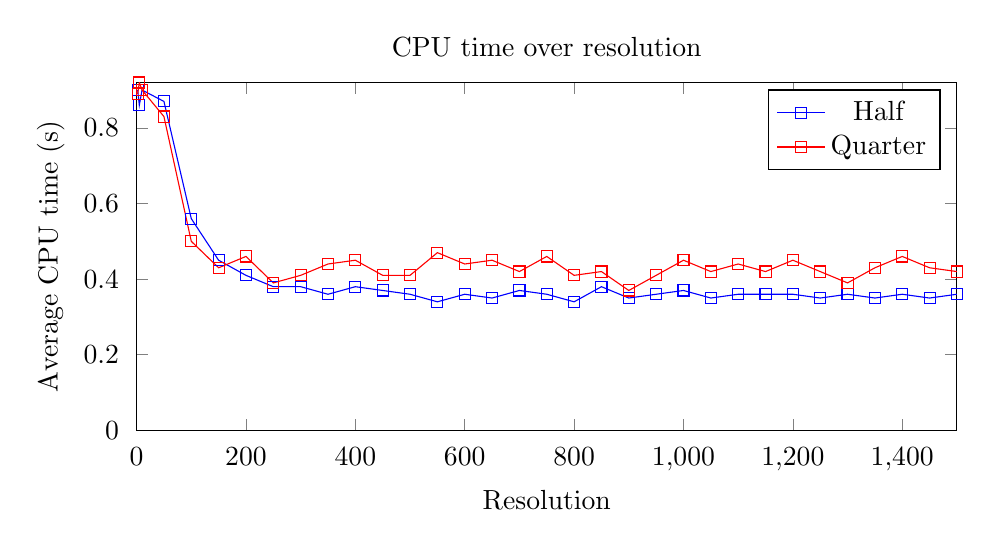
\begin{tikzpicture}
        \begin{axis}[
            width=12cm,
            height=6cm,
            title={CPU time over resolution},
            xlabel={Resolution},
            ylabel={Average CPU time (s)},
            xmin=0,
            ymin=0,
            enlargelimits=false,
            xticklabel shift={.1cm},
            yticklabel shift={.1cm} ]
        ]

        \addplot[
            color=blue,
            mark=square,
            ]
            coordinates {
                (2,0.90)(5,0.86)(10,0.90)(50,0.87)(100,0.56)(150,0.45)(200,0.41)(250,0.38)(300,0.38)(350,0.36)(400,0.38)(450,0.37)(500,0.36)(550,0.34)(600,0.36)(650,0.35)(700,0.37)(750,0.36)(800,0.34)(850,0.38)(900,0.35)(950,0.36)(1000,0.37)(1050,0.35)(1100,0.36)(1150,0.36)(1200,0.36)(1250,0.35)(1300,0.36)(1350,0.35)(1400,0.36)(1450,0.35)(1500,0.36)
            };
            \addlegendentry{Half}
        \addplot[
            color=red,
            mark=square,
            ]
            coordinates {
                (2,0.89)(5,0.92)(10,0.90)(50,0.83)(100,0.50)(150,0.43)(200,0.46)(250,0.39)(300,0.41)(350,0.44)(400,0.45)(450,0.41)(500,0.41)(550,0.47)(600,0.44)(650,0.45)(700,0.42)(750,0.46)(800,0.41)(850,0.42)(900,0.37)(950,0.41)(1000,0.45)(1050,0.42)(1100,0.44)(1150,0.42)(1200,0.45)(1250,0.42)(1300,0.39)(1350,0.43)(1400,0.46)(1450,0.43)(1500,0.42)
            };
            \addlegendentry{Quarter}
        \end{axis}
        \end{tikzpicture}
    \end{center}
    \caption{Performance metrics of the $(1 + 1)$ NA algorithm on the \textit{Half} and \texit{Quarter} benchmarks, with a single neuron, over different resolutions.
    The evolution stopped when the fitness was $2\%$ away from the maximal fitness of $1.0$. The maximum number of iterations was set to $200$.}
    \label{fig:na_maxiter}
\end{figure}

\begin{figure}
    \begin{center}
        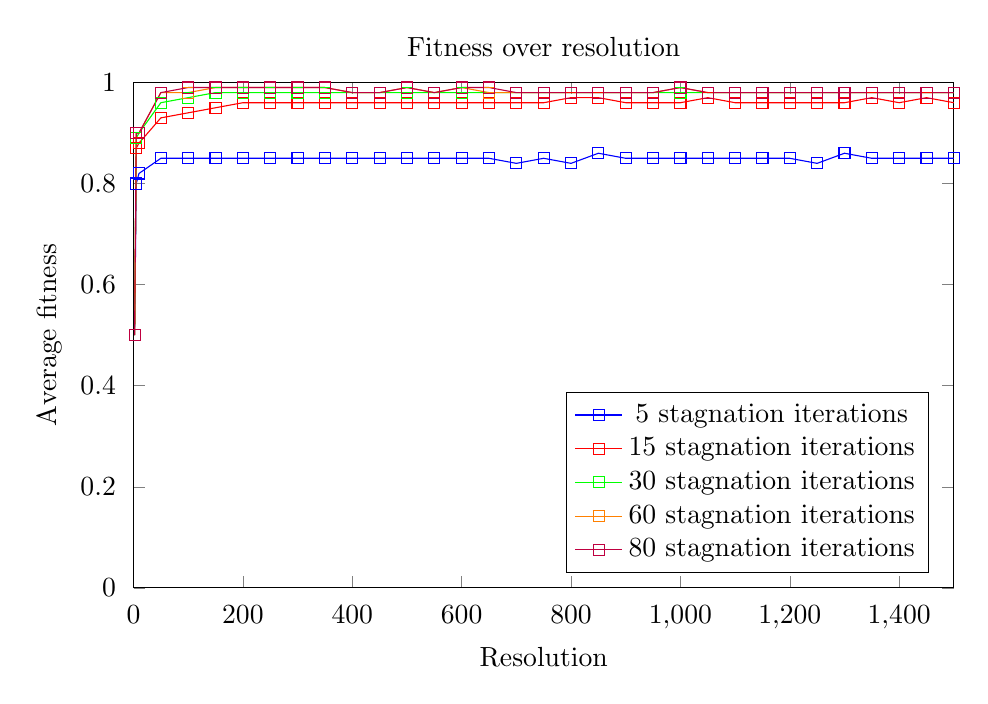
\begin{tikzpicture}
        \begin{axis}[
            width=12cm,
            height=8cm,
            title={Fitness over resolution},
            xlabel={Resolution},
            ylabel={Average fitness},
            enlargelimits=false,
            legend pos=south east,
            xmin=0,
            ymin=0, ymax=1,
            ytick={0,0.2,...,1},
            xticklabel shift={.1cm},
            yticklabel shift={.1cm} ]
        ]

        \addplot[
            color=blue,
            mark=square,
            ]
            coordinates {
                (2,0.50)(5,0.80)(10,0.82)(50,0.85)(100,0.85)(150,0.85)(200,0.85)(250,0.85)(300,0.85)(350,0.85)(400,0.85)(450,0.85)(500,0.85)(550,0.85)(600,0.85)(650,0.85)(700,0.84)(750,0.85)(800,0.84)(850,0.86)(900,0.85)(950,0.85)(1000,0.85)(1050,0.85)(1100,0.85)(1150,0.85)(1200,0.85)(1250,0.84)(1300,0.86)(1350,0.85)(1400,0.85)(1450,0.85)(1500,0.85)
            };
            \addlegendentry{5 stagnation iterations}
        \addplot[
            color=red,
            mark=square,
            ]
            coordinates {
                (2,0.50)(5,0.87)(10,0.88)(50,0.93)(100,0.94)(150,0.95)(200,0.96)(250,0.96)(300,0.96)(350,0.96)(400,0.96)(450,0.96)(500,0.96)(550,0.96)(600,0.96)(650,0.96)(700,0.96)(750,0.96)(800,0.97)(850,0.97)(900,0.96)(950,0.96)(1000,0.96)(1050,0.97)(1100,0.96)(1150,0.96)(1200,0.96)(1250,0.96)(1300,0.96)(1350,0.97)(1400,0.96)(1450,0.97)(1500,0.96)
            };
            \addlegendentry{15 stagnation iterations}
        \addplot[
            color=green,
            mark=square,
            ]
            coordinates {
                (2,0.50)(5,0.89)(10,0.90)(50,0.96)(100,0.97)(150,0.98)(200,0.98)(250,0.98)(300,0.98)(350,0.98)(400,0.98)(450,0.98)(500,0.98)(550,0.98)(600,0.98)(650,0.98)(700,0.98)(750,0.98)(800,0.98)(850,0.98)(900,0.98)(950,0.98)(1000,0.98)(1050,0.98)(1100,0.98)(1150,0.98)(1200,0.98)(1250,0.98)(1300,0.98)(1350,0.98)(1400,0.98)(1450,0.98)(1500,0.98)
            };
            \addlegendentry{30 stagnation iterations}
        \addplot[
            color=orange,
            mark=square,
            ]
            coordinates {
                (2,0.50)(5,0.90)(10,0.90)(50,0.98)(100,0.98)(150,0.99)(200,0.99)(250,0.99)(300,0.99)(350,0.99)(400,0.98)(450,0.98)(500,0.99)(550,0.98)(600,0.99)(650,0.98)(700,0.98)(750,0.98)(800,0.98)(850,0.98)(900,0.98)(950,0.98)(1000,0.99)(1050,0.98)(1100,0.98)(1150,0.98)(1200,0.98)(1250,0.98)(1300,0.98)(1350,0.98)(1400,0.98)(1450,0.98)(1500,0.98)
            };
            \addlegendentry{60 stagnation iterations}
        \addplot[
            color=purple,
            mark=square,
            ]
            coordinates {
                (2,0.50)(5,0.90)(10,0.90)(50,0.98)(100,0.99)(150,0.99)(200,0.99)(250,0.99)(300,0.99)(350,0.99)(400,0.98)(450,0.98)(500,0.99)(550,0.98)(600,0.99)(650,0.99)(700,0.98)(750,0.98)(800,0.98)(850,0.98)(900,0.98)(950,0.98)(1000,0.99)(1050,0.98)(1100,0.98)(1150,0.98)(1200,0.98)(1250,0.98)(1300,0.98)(1350,0.98)(1400,0.98)(1450,0.98)(1500,0.98)
            };
            \addlegendentry{80 stagnation iterations}
        \end{axis}
        \end{tikzpicture}
        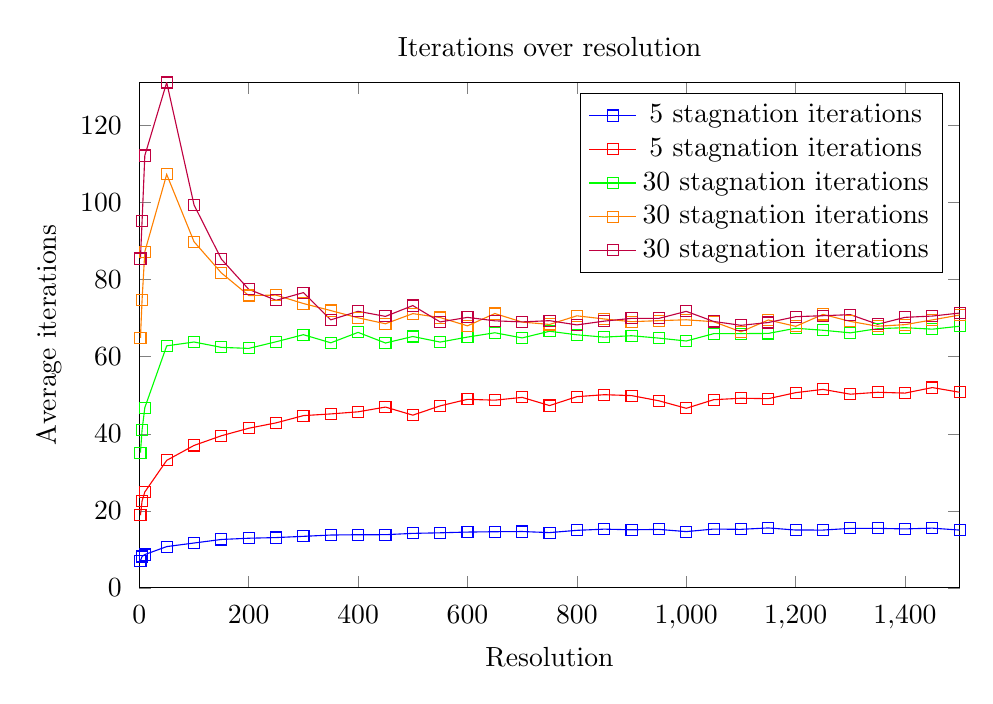
\begin{tikzpicture}
        \begin{axis}[
            width=12cm,
            height=8cm,
            title={Iterations over resolution},
            xlabel={Resolution},
            ylabel={Average iterations},
            xmin=0,
            ymin=0,
            enlargelimits=false,
            xticklabel shift={.1cm},
            yticklabel shift={.1cm} ]
        ]

        \addplot[
            color=blue,
            mark=square,
            ]
            coordinates {
                (2,7.06)(5,8.15)(10,8.65)(50,10.72)(100,11.65)(150,12.57)(200,12.89)(250,13.06)(300,13.38)(350,13.72)(400,13.80)(450,13.81)(500,14.15)(550,14.30)(600,14.49)(650,14.58)(700,14.63)(750,14.35)(800,14.94)(850,15.25)(900,15.08)(950,15.18)(1000,14.61)(1050,15.27)(1100,15.20)(1150,15.56)(1200,15.02)(1250,15.01)(1300,15.45)(1350,15.45)(1400,15.31)(1450,15.51)(1500,15.00)
            };
            \addlegendentry{5 stagnation iterations}
        \addplot[
            color=red,
            mark=square,
            ]
            coordinates {
                (2,18.86)(5,22.58)(10,24.90)(50,33.10)(100,36.98)(150,39.49)(200,41.44)(250,42.84)(300,44.72)(350,45.16)(400,45.71)(450,46.94)(500,44.84)(550,47.25)(600,48.95)(650,48.73)(700,49.45)(750,47.33)(800,49.64)(850,50.15)(900,49.92)(950,48.57)(1000,46.62)(1050,48.85)(1100,49.23)(1150,49.12)(1200,50.68)(1250,51.53)(1300,50.28)(1350,50.78)(1400,50.57)(1450,52.00)(1500,50.78)
            };
            \addlegendentry{5 stagnation iterations}
        \addplot[
            color=green,
            mark=square,
            ]
            coordinates {
                (2,35.10)(5,41.03)(10,46.80)(50,62.83)(100,63.83)(150,62.44)(200,62.17)(250,63.89)(300,65.73)(350,63.62)(400,66.33)(450,63.57)(500,65.26)(550,63.81)(600,65.11)(650,66.23)(700,64.89)(750,66.62)(800,65.70)(850,65.10)(900,65.46)(950,64.84)(1000,64.09)(1050,65.99)(1100,66.01)(1150,66.06)(1200,67.40)(1250,66.88)(1300,66.21)(1350,67.29)(1400,67.55)(1450,67.16)(1500,67.93)
            };
            \addlegendentry{30 stagnation iterations}
        \addplot[
            color=orange,
            mark=square,
            ]
            coordinates {
                (2,64.93)(5,74.80)(10,87.27)(50,107.34)(100,89.86)(150,81.76)(200,75.90)(250,75.99)(300,73.82)(350,71.99)(400,70.11)(450,68.57)(500,71.20)(550,70.18)(600,68.02)(650,71.22)(700,69.00)(750,68.39)(800,70.63)(850,69.81)(900,69.11)(950,69.37)(1000,69.60)(1050,69.10)(1100,66.48)(1150,69.54)(1200,67.90)(1250,70.99)(1300,69.18)(1350,67.92)(1400,68.34)(1450,69.57)(1500,70.84)
            };
            \addlegendentry{30 stagnation iterations}
        \addplot[
            color=purple,
            mark=square,
            ]
            coordinates {
                (2,85.50)(5,95.21)(10,112.23)(50,131.20)(100,99.42)(150,85.34)(200,77.51)(250,74.66)(300,76.65)(350,69.58)(400,71.80)(450,70.48)(500,73.29)(550,69.04)(600,70.22)(650,69.33)(700,69.05)(750,69.37)(800,68.27)(850,69.25)(900,69.97)(950,69.96)(1000,71.79)(1050,69.17)(1100,68.16)(1150,68.89)(1200,70.40)(1250,70.66)(1300,70.93)(1350,68.44)(1400,70.23)(1450,70.57)(1500,71.35)
            };
            \addlegendentry{30 stagnation iterations}
        \end{axis}
        \end{tikzpicture}
    \end{center}
    \caption{Performance metrics of the $(1 + 1)$ NA algorithm on the \textit{Half} benchmark, with a single neuron, over different resolutions.
    The evolution stopped when the fitness was $2\%$ away from the maximal fitness of $1.0$ or the maximum number of stagnation iteration was reached.}
    \label{fig:na_half_stagnation}
\end{figure}

\begin{figure}
    \begin{center}
        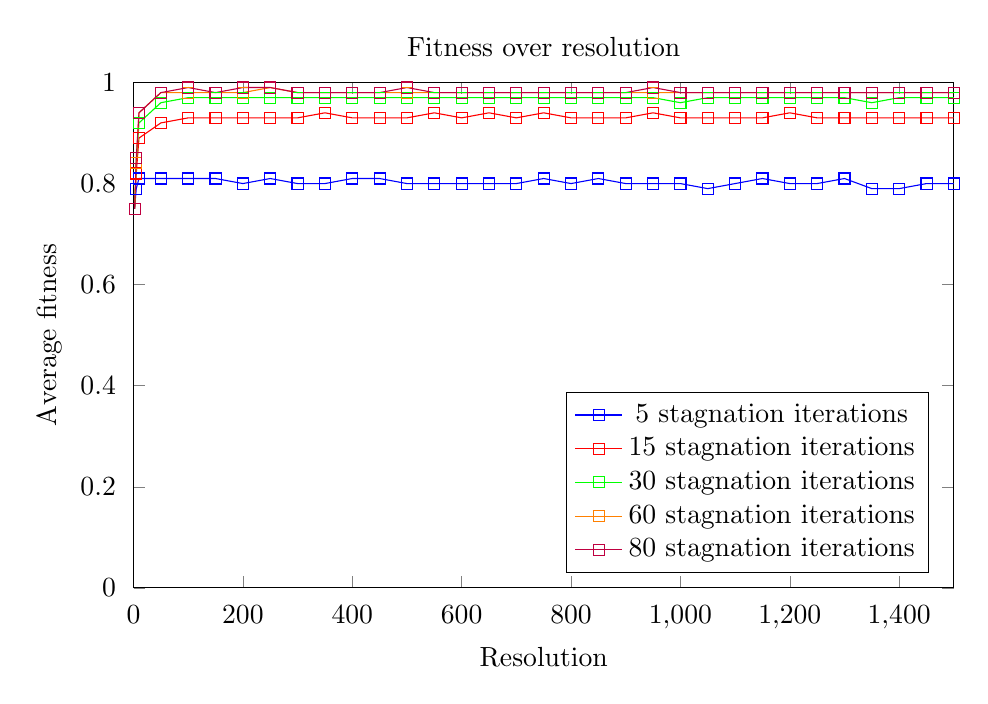
\begin{tikzpicture}
        \begin{axis}[
            width=12cm,
            height=8cm,
            title={Fitness over resolution},
            xlabel={Resolution},
            ylabel={Average fitness},
            enlargelimits=false,
            legend pos=south east,
            xmin=0,
            ymin=0, ymax=1,
            ytick={0,0.2,...,1},
            xticklabel shift={.1cm},
            yticklabel shift={.1cm} ]
        ]

        \addplot[
            color=blue,
            mark=square,
            ]
            coordinates {
                (2,0.75)(5,0.79)(10,0.81)(50,0.81)(100,0.81)(150,0.81)(200,0.80)(250,0.81)(300,0.80)(350,0.80)(400,0.81)(450,0.81)(500,0.80)(550,0.80)(600,0.80)(650,0.80)(700,0.80)(750,0.81)(800,0.80)(850,0.81)(900,0.80)(950,0.80)(1000,0.80)(1050,0.79)(1100,0.80)(1150,0.81)(1200,0.80)(1250,0.80)(1300,0.81)(1350,0.79)(1400,0.79)(1450,0.80)(1500,0.80)
            };
            \addlegendentry{5 stagnation iterations}
        \addplot[
            color=red,
            mark=square,
            ]
            coordinates {
                (2,0.75)(5,0.82)(10,0.89)(50,0.92)(100,0.93)(150,0.93)(200,0.93)(250,0.93)(300,0.93)(350,0.94)(400,0.93)(450,0.93)(500,0.93)(550,0.94)(600,0.93)(650,0.94)(700,0.93)(750,0.94)(800,0.93)(850,0.93)(900,0.93)(950,0.94)(1000,0.93)(1050,0.93)(1100,0.93)(1150,0.93)(1200,0.94)(1250,0.93)(1300,0.93)(1350,0.93)(1400,0.93)(1450,0.93)(1500,0.93)
            };
            \addlegendentry{15 stagnation iterations}
        \addplot[
            color=green,
            mark=square,
            ]
            coordinates {
                (2,0.75)(5,0.84)(10,0.92)(50,0.96)(100,0.97)(150,0.97)(200,0.97)(250,0.97)(300,0.97)(350,0.97)(400,0.97)(450,0.97)(500,0.97)(550,0.97)(600,0.97)(650,0.97)(700,0.97)(750,0.97)(800,0.97)(850,0.97)(900,0.97)(950,0.97)(1000,0.96)(1050,0.97)(1100,0.97)(1150,0.97)(1200,0.97)(1250,0.97)(1300,0.97)(1350,0.96)(1400,0.97)(1450,0.97)(1500,0.97)
            };
            \addlegendentry{30 stagnation iterations}
        \addplot[
            color=orange,
            mark=square,
            ]
            coordinates {
                (2,0.75)(5,0.84)(10,0.94)(50,0.98)(100,0.98)(150,0.98)(200,0.98)(250,0.99)(300,0.98)(350,0.98)(400,0.98)(450,0.98)(500,0.98)(550,0.98)(600,0.98)(650,0.98)(700,0.98)(750,0.98)(800,0.98)(850,0.98)(900,0.98)(950,0.98)(1000,0.98)(1050,0.98)(1100,0.98)(1150,0.98)(1200,0.98)(1250,0.98)(1300,0.98)(1350,0.98)(1400,0.98)(1450,0.98)(1500,0.98)
            };
            \addlegendentry{60 stagnation iterations}
        \addplot[
            color=purple,
            mark=square,
            ]
            coordinates {
                (2,0.75)(5,0.85)(10,0.94)(50,0.98)(100,0.99)(150,0.98)(200,0.99)(250,0.99)(300,0.98)(350,0.98)(400,0.98)(450,0.98)(500,0.99)(550,0.98)(600,0.98)(650,0.98)(700,0.98)(750,0.98)(800,0.98)(850,0.98)(900,0.98)(950,0.99)(1000,0.98)(1050,0.98)(1100,0.98)(1150,0.98)(1200,0.98)(1250,0.98)(1300,0.98)(1350,0.98)(1400,0.98)(1450,0.98)(1500,0.98)
            };
            \addlegendentry{80 stagnation iterations}
        \end{axis}
        \end{tikzpicture}
        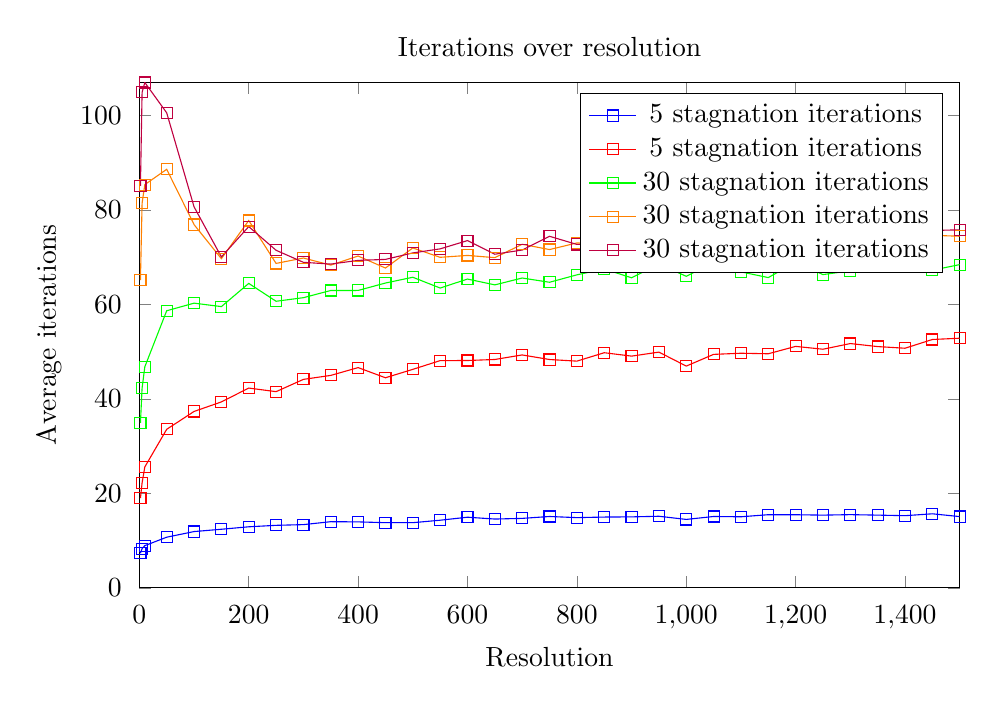
\begin{tikzpicture}
        \begin{axis}[
            width=12cm,
            height=8cm,
            title={Iterations over resolution},
            xlabel={Resolution},
            ylabel={Average iterations},
            xmin=0,
            ymin=0,
            enlargelimits=false,
            xticklabel shift={.1cm},
            yticklabel shift={.1cm} ]
        ]

        \addplot[
            color=blue,
            mark=square,
            ]
            coordinates {
                (2,7.32)(5,8.31)(10,8.94)(50,10.73)(100,11.92)(150,12.41)(200,12.93)(250,13.24)(300,13.39)(350,14.01)(400,13.97)(450,13.80)(500,13.80)(550,14.32)(600,14.96)(650,14.57)(700,14.71)(750,15.11)(800,14.87)(850,14.99)(900,15.03)(950,15.16)(1000,14.49)(1050,15.11)(1100,15.05)(1150,15.49)(1200,15.48)(1250,15.40)(1300,15.50)(1350,15.40)(1400,15.28)(1450,15.68)(1500,15.09)
            };
            \addlegendentry{5 stagnation iterations}
        \addplot[
            color=red,
            mark=square,
            ]
            coordinates {
                (2,19.01)(5,22.21)(10,25.60)(50,33.56)(100,37.34)(150,39.36)(200,42.29)(250,41.53)(300,44.13)(350,44.97)(400,46.62)(450,44.47)(500,46.25)(550,48.10)(600,48.12)(650,48.34)(700,49.30)(750,48.33)(800,47.99)(850,49.77)(900,49.05)(950,49.90)(1000,46.94)(1050,49.42)(1100,49.66)(1150,49.55)(1200,51.11)(1250,50.51)(1300,51.71)(1350,51.07)(1400,50.72)(1450,52.57)(1500,52.84)
            };
            \addlegendentry{5 stagnation iterations}
        \addplot[
            color=green,
            mark=square,
            ]
            coordinates {
                (2,34.90)(5,42.26)(10,46.79)(50,58.65)(100,60.26)(150,59.53)(200,64.44)(250,60.66)(300,61.42)(350,62.94)(400,62.95)(450,64.52)(500,65.74)(550,63.46)(600,65.36)(650,64.13)(700,65.58)(750,64.68)(800,66.25)(850,67.50)(900,65.62)(950,68.56)(1000,65.94)(1050,68.91)(1100,66.88)(1150,65.67)(1200,68.95)(1250,66.30)(1300,67.12)(1350,68.57)(1400,68.28)(1450,67.23)(1500,68.42)
            };
            \addlegendentry{30 stagnation iterations}
        \addplot[
            color=orange,
            mark=square,
            ]
            coordinates {
                (2,65.12)(5,81.40)(10,85.35)(50,88.59)(100,76.89)(150,69.67)(200,77.75)(250,68.67)(300,69.81)(350,68.31)(400,70.23)(450,67.69)(500,71.94)(550,69.96)(600,70.36)(650,69.89)(700,72.72)(750,71.60)(800,73.00)(850,72.79)(900,70.43)(950,72.85)(1000,73.94)(1050,73.24)(1100,71.88)(1150,70.81)(1200,73.85)(1250,72.48)(1300,72.25)(1350,72.97)(1400,74.65)(1450,74.62)(1500,74.42)
            };
            \addlegendentry{30 stagnation iterations}
        \addplot[
            color=purple,
            mark=square,
            ]
            coordinates {
                (2,85.07)(5,104.87)(10,106.96)(50,100.54)(100,80.65)(150,70.04)(200,76.46)(250,71.45)(300,68.90)(350,68.53)(400,69.31)(450,69.52)(500,70.89)(550,71.75)(600,73.50)(650,70.62)(700,71.50)(750,74.41)(800,72.69)(850,72.92)(900,73.98)(950,70.70)(1000,76.71)(1050,73.13)(1100,73.70)(1150,76.53)(1200,71.96)(1250,75.06)(1300,73.11)(1350,76.36)(1400,77.01)(1450,75.64)(1500,75.78)
            };
            \addlegendentry{30 stagnation iterations}
        \end{axis}
        \end{tikzpicture}
    \end{center}
    \caption{Performance metrics of the $(1 + 1)$ NA algorithm on the \textit{Quarter} benchmark, with a single neuron, over different resolutions.
    The evolution stopped when the fitness was $2\%$ away from the maximal fitness of $1.0$ or the maximum number of stagnation iteration was reached.}
    \label{fig:na_quarter_stagnation}
\end{figure}

\begin{figure}
    \begin{center}
        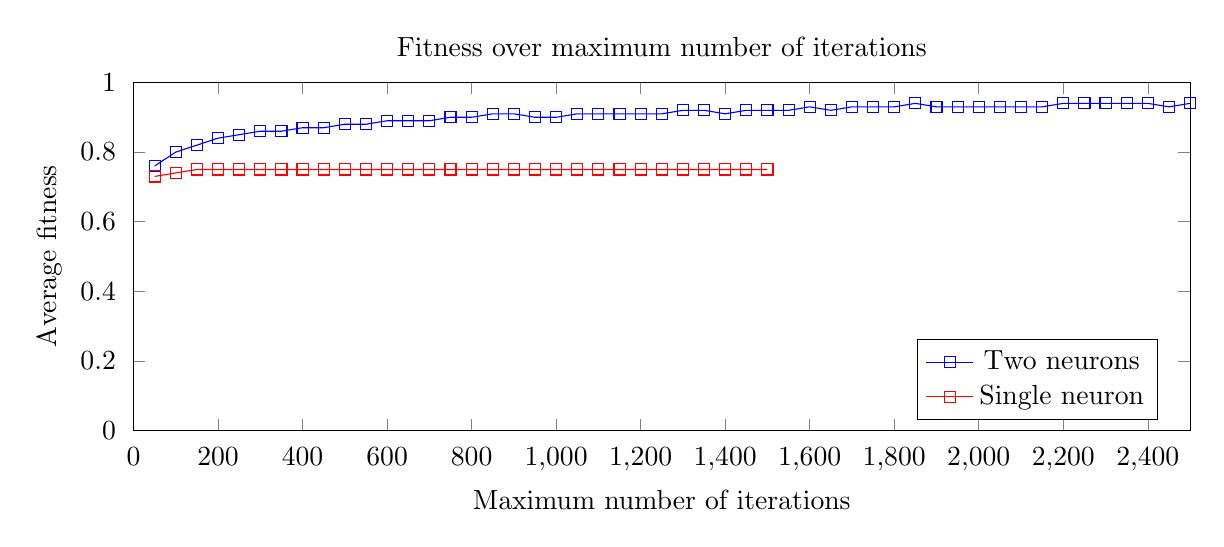
\begin{tikzpicture}
        \begin{axis}[
            width=15cm,
            height=6cm,
            title={Fitness over maximum number of iterations},
            legend pos=south east,
            xlabel={Maximum number of iterations},
            ylabel={Average fitness},
            enlargelimits=false,
            xmin=0,
            ymin=0, ymax=1,
            ytick={0,0.2,...,1},
            xticklabel shift={.1cm},
            yticklabel shift={.1cm} ]
        ]

        \addplot[
            color=blue,
            mark=square,
            ]
            coordinates {
                (50,0.76)(100,0.80)(150,0.82)(200,0.84)(250,0.85)(300,0.86)(350,0.86)(400,0.87)(450,0.87)(500,0.88)(550,0.88)(600,0.89)(650,0.89)(700,0.89)(750,0.90)(800,0.90)(850,0.91)(900,0.91)(950,0.90)(1000,0.90)(1050,0.91)(1100,0.91)(1150,0.91)(1200,0.91)(1250,0.91)(1300,0.92)(1350,0.92)(1400,0.91)(1450,0.92)(1500,0.92)(1550,0.92)(1600,0.93)(1650,0.92)(1700,0.93)(1750,0.93)(1800,0.93)(1850,0.94)(1900,0.93)(1950,0.93)(2000,0.93)(2050,0.93)(2100,0.93)(2150,0.93)(2200,0.94)(2250,0.94)(2300,0.94)(2350,0.94)(2400,0.94)(2450,0.93)(2500,0.94)
            };
            \addlegendentry{Two neurons}
        \addplot[
            color=red,
            mark=square,
            ]
            coordinates {
                (50,0.73)(100,0.74)(150,0.75)(200,0.75)(250,0.75)(300,0.75)(350,0.75)(400,0.75)(450,0.75)(500,0.75)(550,0.75)(600,0.75)(650,0.75)(700,0.75)(750,0.75)(800,0.75)(850,0.75)(900,0.75)(950,0.75)(1000,0.75)(1050,0.75)(1100,0.75)(1150,0.75)(1200,0.75)(1250,0.75)(1300,0.75)(1350,0.75)(1400,0.75)(1450,0.75)(1500,0.75)
            };
            \addlegendentry{Single neuron}
        \end{axis}
        \end{tikzpicture}
        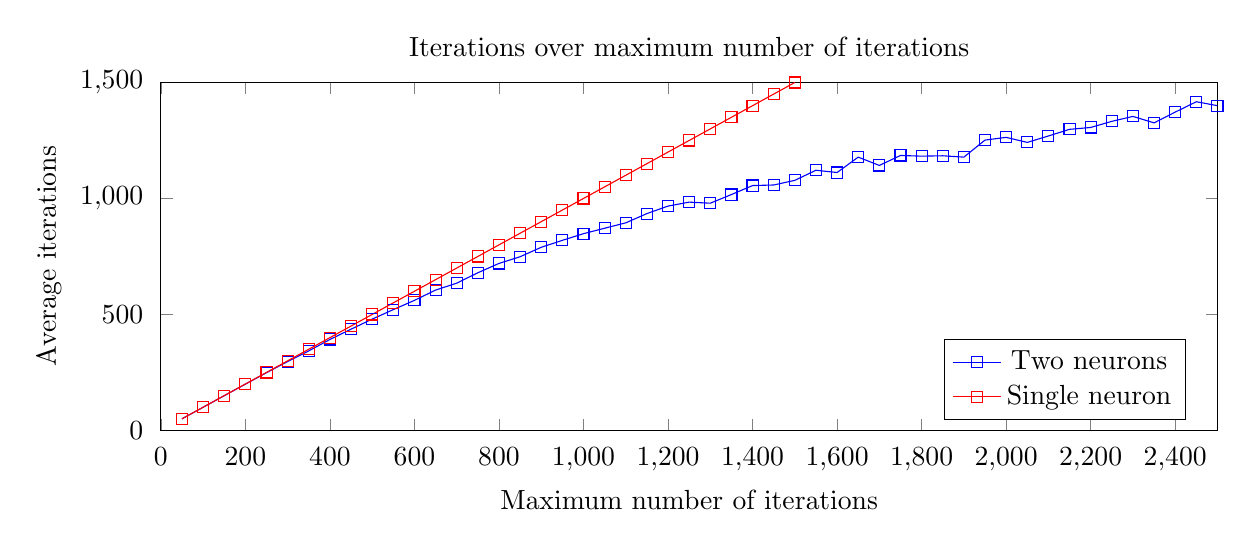
\begin{tikzpicture}
        \begin{axis}[
            width=15cm,
            height=6cm,
            legend pos=south east,
            title={Iterations over maximum number of iterations},
            xlabel={Maximum number of iterations},
            ylabel={Average iterations},
            xmin=0,
            ymin=0,
            enlargelimits=false,
            xticklabel shift={.1cm},
            yticklabel shift={.1cm} ]
        ]

        \addplot[
            color=blue,
            mark=square,
            ]
            coordinates {
                (50,49.97)(100,99.88)(150,149.73)(200,199.47)(250,248.90)(300,296.92)(350,342.93)(400,392.04)(450,436.46)(500,479.91)(550,520.86)(600,560.64)(650,604.99)(700,634.84)(750,679.66)(800,719.92)(850,748.80)(900,789.45)(950,819.47)(1000,848.19)(1050,871.68)(1100,894.90)(1150,934.78)(1200,967.18)(1250,984.16)(1300,979.59)(1350,1016.89)(1400,1055.63)(1450,1058.06)(1500,1078.15)(1550,1121.60)(1600,1111.85)(1650,1178.21)(1700,1142.42)(1750,1185.41)(1800,1182.37)(1850,1184.01)(1900,1178.17)(1950,1251.66)(2000,1263.44)(2050,1241.68)(2100,1269.41)(2150,1298.02)(2200,1306.06)(2250,1332.45)(2300,1353.79)(2350,1325.92)(2400,1372.23)(2450,1417.02)(2500,1400.06)
            };
            \addlegendentry{Two neurons}
        \addplot[
            color=red,
            mark=square,
            ]
            coordinates {
                (50,50.00)(100,100.00)(150,150.00)(200,200.00)(250,250.00)(300,300.00)(350,350.00)(400,400.00)(450,450.00)(500,500.00)(550,550.00)(600,600.00)(650,650.00)(700,700.00)(750,750.00)(800,800.00)(850,850.00)(900,900.00)(950,950.00)(1000,1000.00)(1050,1050.00)(1100,1100.00)(1150,1150.00)(1200,1200.00)(1250,1250.00)(1300,1300.00)(1350,1350.00)(1400,1400.00)(1450,1450.00)(1500,1500.00)
            };
            \addlegendentry{Single neuron}
        \end{axis}
        \end{tikzpicture}
        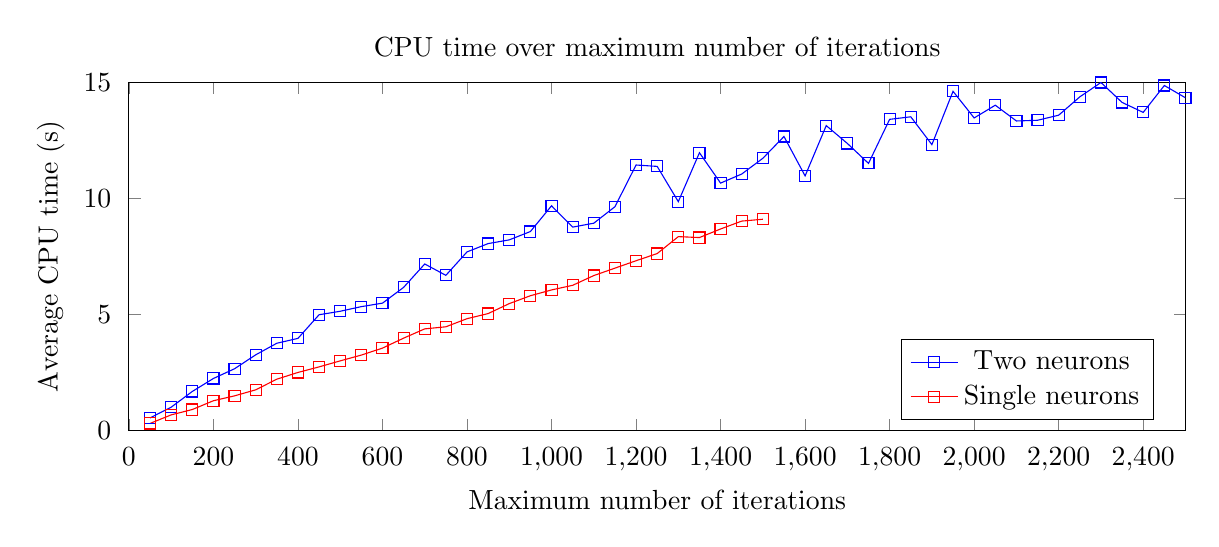
\begin{tikzpicture}
        \begin{axis}[
            width=15cm,
            height=6cm,
            legend pos=south east,
            title={CPU time over maximum number of iterations},
            xlabel={Maximum number of iterations},
            ylabel={Average CPU time (s)},
            xmin=0,
            ymin=0,
            enlargelimits=false,
            xticklabel shift={.1cm},
            yticklabel shift={.1cm} ]
        ]

        \addplot[
            color=blue,
            mark=square,
            ]
            coordinates {
                (50,0.54)(100,1.00)(150,1.68)(200,2.24)(250,2.66)(300,3.26)(350,3.76)(400,3.97)(450,4.99)(500,5.14)(550,5.34)(600,5.49)(650,6.17)(700,7.18)(750,6.69)(800,7.70)(850,8.06)(900,8.22)(950,8.58)(1000,9.69)(1050,8.77)(1100,8.94)(1150,9.65)(1200,11.45)(1250,11.39)(1300,9.87)(1350,11.98)(1400,10.67)(1450,11.06)(1500,11.74)(1550,12.68)(1600,10.98)(1650,13.15)(1700,12.38)(1750,11.52)(1800,13.42)(1850,13.53)(1900,12.33)(1950,14.63)(2000,13.48)(2050,14.03)(2100,13.35)(2150,13.38)(2200,13.60)(2250,14.39)(2300,15.01)(2350,14.15)(2400,13.72)(2450,14.88)(2500,14.35)
            };
            \addlegendentry{Two neurons}
        \addplot[
            color=red,
            mark=square,
            ]
            coordinates {
                (50,0.30)(100,0.67)(150,0.90)(200,1.28)(250,1.49)(300,1.75)(350,2.21)(400,2.50)(450,2.74)(500,3.00)(550,3.25)(600,3.55)(650,3.98)(700,4.38)(750,4.47)(800,4.82)(850,5.04)(900,5.47)(950,5.81)(1000,6.06)(1050,6.26)(1100,6.68)(1150,7.00)(1200,7.32)(1250,7.63)(1300,8.36)(1350,8.32)(1400,8.69)(1450,9.03)(1500,9.11)
            };
            \addlegendentry{Single neurons}
        \end{axis}
        \end{tikzpicture}
    \end{center}
    \caption{Performance metrics of the $(1 + 1)$ NA algorithm on the \textit{TwoQuarters} benchmark, over different maximum iterations.
    The evolution stopped when the fitness was $2\%$ away from the maximal fitness of $1.0$ or the maximum number of iterations was reached.}
    \label{fig:na_twoquarters}
\end{figure}

\begin{figure}
    \begin{center}
        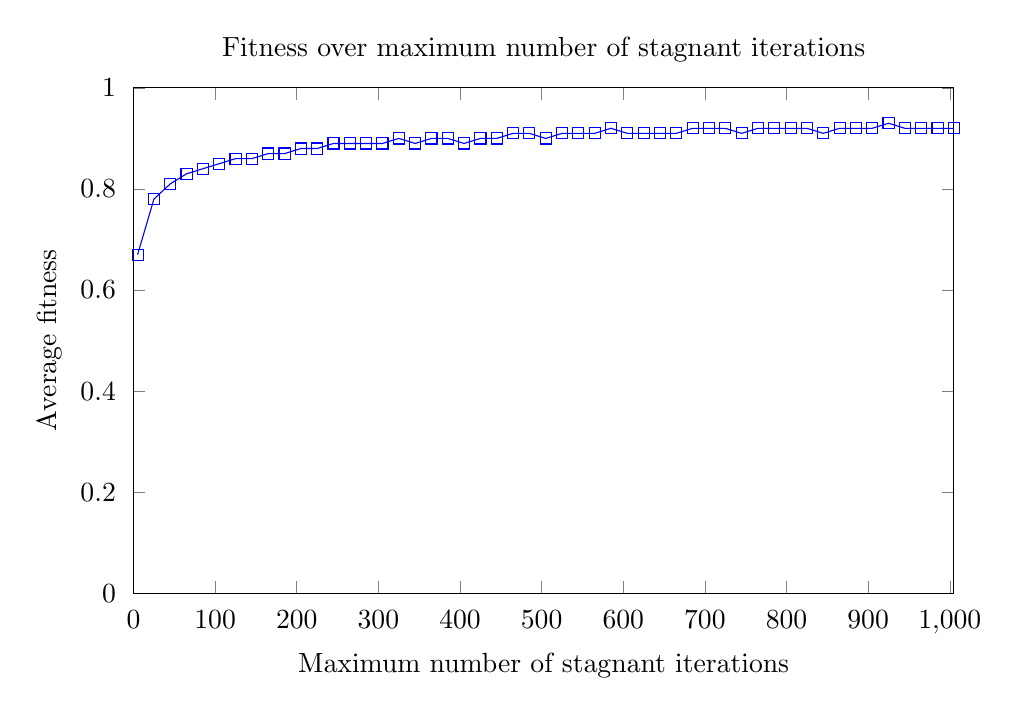
\begin{tikzpicture}
        \begin{axis}[
            width=12cm,
            height=8cm,
            title={Fitness over maximum number of stagnant iterations},
            xlabel={Maximum number of stagnant iterations},
            ylabel={Average fitness},
            enlargelimits=false,
            xmin=0,
            ymin=0, ymax=1,
            ytick={0,0.2,...,1},
            xticklabel shift={.1cm},
            yticklabel shift={.1cm} ]
        ]

        \addplot[
            color=blue,
            mark=square,
            ]
            coordinates {
                (5,0.67)(25,0.78)(45,0.81)(65,0.83)(85,0.84)(105,0.85)(125,0.86)(145,0.86)(165,0.87)(185,0.87)(205,0.88)(225,0.88)(245,0.89)(265,0.89)(285,0.89)(305,0.89)(325,0.90)(345,0.89)(365,0.90)(385,0.90)(405,0.89)(425,0.90)(445,0.90)(465,0.91)(485,0.91)(505,0.90)(525,0.91)(545,0.91)(565,0.91)(585,0.92)(605,0.91)(625,0.91)(645,0.91)(665,0.91)(685,0.92)(705,0.92)(725,0.92)(745,0.91)(765,0.92)(785,0.92)(805,0.92)(825,0.92)(845,0.91)(865,0.92)(885,0.92)(905,0.92)(925,0.93)(945,0.92)(965,0.92)(985,0.92)(1005,0.92)
            };
        \end{axis}
        \end{tikzpicture}
        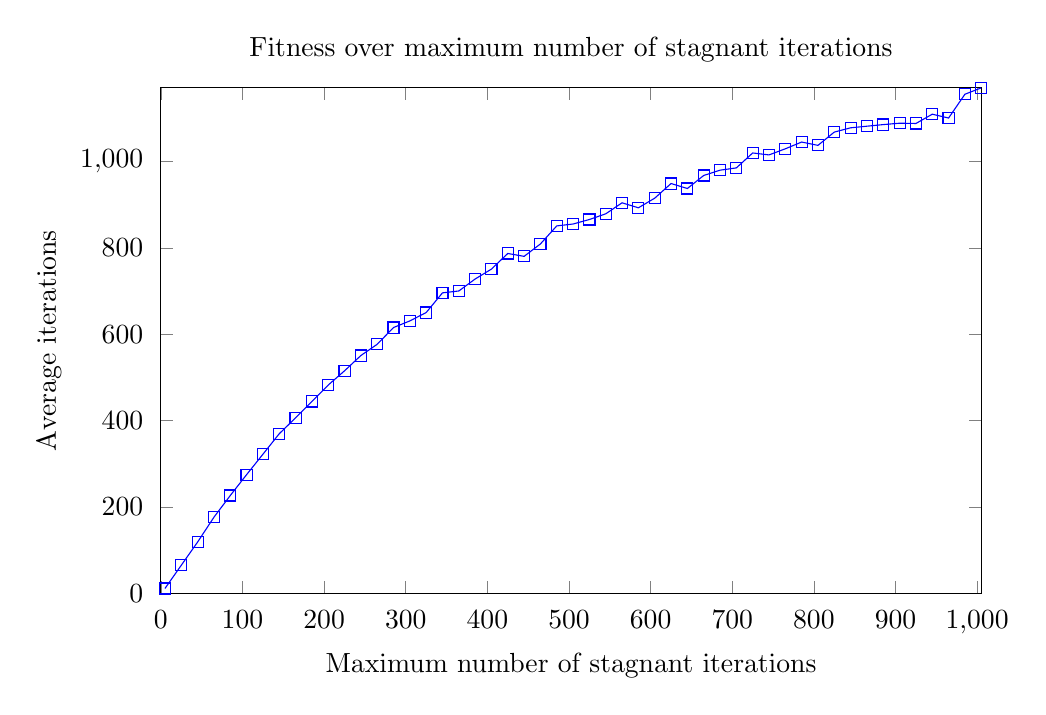
\begin{tikzpicture}
        \begin{axis}[
            width=12cm,
            height=8cm,
            title={Fitness over maximum number of stagnant iterations},
            xlabel={Maximum number of stagnant iterations},
            ylabel={Average iterations},
            xmin=0,
            ymin=0,
            enlargelimits=false,
            xticklabel shift={.1cm},
            yticklabel shift={.1cm} ]
        ]

        \addplot[
            color=blue,
            mark=square,
            ]
            coordinates {
                (5,11.08)(25,64.92)(45,118.66)(65,176.18)(85,226.47)(105,274.75)(125,322.09)(145,369.60)(165,406.29)(185,444.36)(205,482.35)(225,515.39)(245,550.76)(265,576.87)(285,615.67)(305,630.95)(325,650.39)(345,696.00)(365,700.34)(385,728.06)(405,751.11)(425,787.23)(445,780.55)(465,809.38)(485,851.13)(505,855.51)(525,865.96)(545,879.14)(565,904.62)(585,893.06)(605,915.34)(625,949.31)(645,937.78)(665,967.92)(685,980.22)(705,985.50)(725,1020.09)(745,1015.59)(765,1029.75)(785,1045.41)(805,1037.69)(825,1068.49)(845,1078.37)(865,1082.12)(885,1085.85)(905,1089.08)(925,1088.42)(945,1109.95)(965,1101.04)(985,1156.12)(1005,1170.91)
            };
        \end{axis}
        \end{tikzpicture}
    \end{center}
    \caption{Performance metrics of the $(1 + 1)$ NA algorithm on the \textit{TwoQuarters} benchmark with two  neurons, over different numbers of maximum stagnant iterations.
    The evolution stopped when the fitness was $2\%$ away from the maximal fitness of $1.0$, when $2500$ iterations was reached, or the maximum number of stagnant iterations was reached.}
    \label{fig:na_twoquarters_stag}
\end{figure}

\begin{figure}
    \begin{center}
        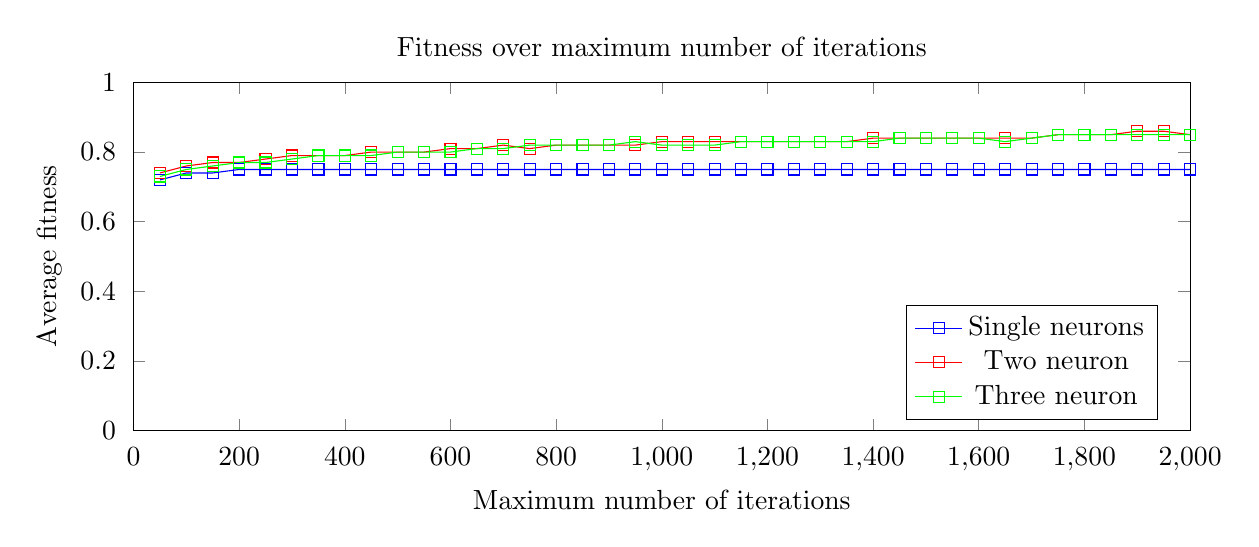
\begin{tikzpicture}
        \begin{axis}[
            width=15cm,
            height=6cm,
            title={Fitness over maximum number of iterations},
            legend pos=south east,
            xlabel={Maximum number of iterations},
            ylabel={Average fitness},
            enlargelimits=false,
            xmin=0,
            ymin=0, ymax=1,
            ytick={0,0.2,...,1},
            xticklabel shift={.1cm},
            yticklabel shift={.1cm} ]
        ]

        \addplot[
            color=blue,
            mark=square,
            ]
            coordinates {
                (50,0.72)(100,0.74)(150,0.74)(200,0.75)(250,0.75)(300,0.75)(350,0.75)(400,0.75)(450,0.75)(500,0.75)(550,0.75)(600,0.75)(650,0.75)(700,0.75)(750,0.75)(800,0.75)(850,0.75)(900,0.75)(950,0.75)(1000,0.75)(1050,0.75)(1100,0.75)(1150,0.75)(1200,0.75)(1250,0.75)(1300,0.75)(1350,0.75)(1400,0.75)(1450,0.75)(1500,0.75)(1550,0.75)(1600,0.75)(1650,0.75)(1700,0.75)(1750,0.75)(1800,0.75)(1850,0.75)(1900,0.75)(1950,0.75)(2000,0.75)
            };
            \addlegendentry{Single neurons}
        \addplot[
            color=red,
            mark=square,
            ]
            coordinates {
                (50,0.74)(100,0.76)(150,0.77)(200,0.77)(250,0.78)(300,0.79)(350,0.79)(400,0.79)(450,0.80)(500,0.80)(550,0.80)(600,0.81)(650,0.81)(700,0.82)(750,0.81)(800,0.82)(850,0.82)(900,0.82)(950,0.82)(1000,0.83)(1050,0.83)(1100,0.83)(1150,0.83)(1200,0.83)(1250,0.83)(1300,0.83)(1350,0.83)(1400,0.84)(1450,0.84)(1500,0.84)(1550,0.84)(1600,0.84)(1650,0.84)(1700,0.84)(1750,0.85)(1800,0.85)(1850,0.85)(1900,0.86)(1950,0.86)(2000,0.85)
            };
            \addlegendentry{Two neuron}
        \addplot[
            color=green,
            mark=square,
            ]
            coordinates {
                (50,0.73)(100,0.75)(150,0.76)(200,0.77)(250,0.77)(300,0.78)(350,0.79)(400,0.79)(450,0.79)(500,0.80)(550,0.80)(600,0.80)(650,0.81)(700,0.81)(750,0.82)(800,0.82)(850,0.82)(900,0.82)(950,0.83)(1000,0.82)(1050,0.82)(1100,0.82)(1150,0.83)(1200,0.83)(1250,0.83)(1300,0.83)(1350,0.83)(1400,0.83)(1450,0.84)(1500,0.84)(1550,0.84)(1600,0.84)(1650,0.83)(1700,0.84)(1750,0.85)(1800,0.85)(1850,0.85)(1900,0.85)(1950,0.85)(2000,0.85)
            };
            \addlegendentry{Three neuron}
        \end{axis}
        \end{tikzpicture}
        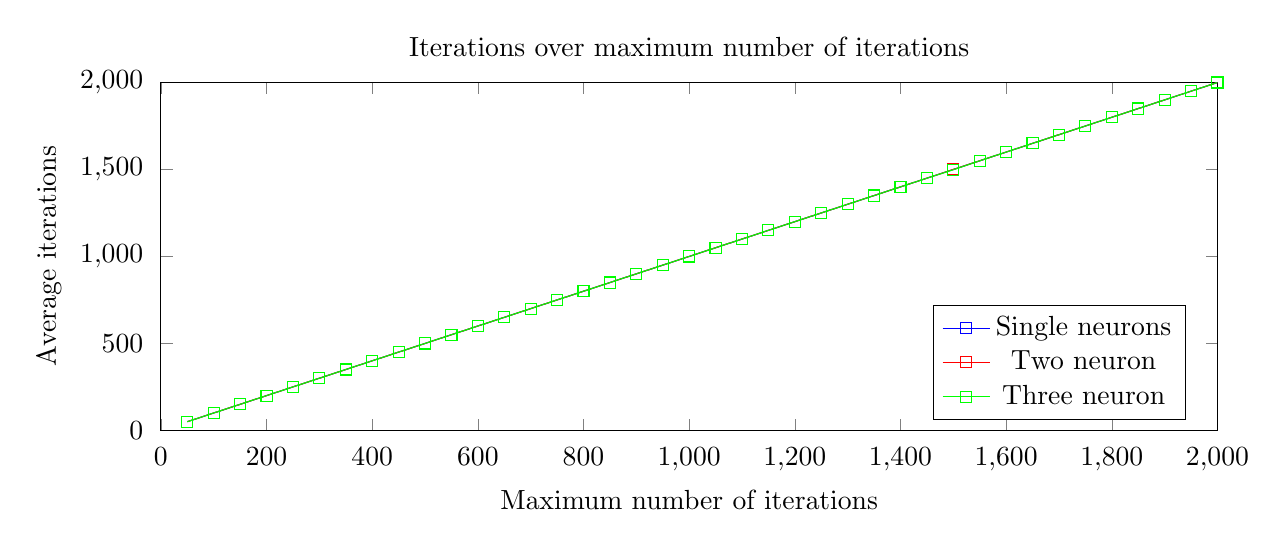
\begin{tikzpicture}
        \begin{axis}[
            width=15cm,
            height=6cm,
            legend pos=south east,
            title={Iterations over maximum number of iterations},
            xlabel={Maximum number of iterations},
            ylabel={Average iterations},
            xmin=0,
            ymin=0,
            enlargelimits=false,
            xticklabel shift={.1cm},
            yticklabel shift={.1cm} ]
        ]

        \addplot[
            color=blue,
            mark=square,
            ]
            coordinates {
                (50,50.00)(100,100.00)(150,150.00)(200,200.00)(250,250.00)(300,300.00)(350,350.00)(400,400.00)(450,450.00)(500,500.00)(550,550.00)(600,600.00)(650,650.00)(700,700.00)(750,750.00)(800,800.00)(850,850.00)(900,900.00)(950,950.00)(1000,1000.00)(1050,1050.00)(1100,1100.00)(1150,1150.00)(1200,1200.00)(1250,1250.00)(1300,1300.00)(1350,1350.00)(1400,1400.00)(1450,1450.00)(1500,1500.00)(1550,1550.00)(1600,1600.00)(1650,1650.00)(1700,1700.00)(1750,1750.00)(1800,1800.00)(1850,1850.00)(1900,1900.00)(1950,1950.00)(2000,2000.00)
            };
            \addlegendentry{Single neurons}
        \addplot[
            color=red,
            mark=square,
            ]
            coordinates {
                (50,50.00)(100,100.00)(150,150.00)(200,200.00)(250,250.00)(300,300.00)(350,350.00)(400,400.00)(450,450.00)(500,500.00)(550,550.00)(600,600.00)(650,650.00)(700,700.00)(750,750.00)(800,800.00)(850,850.00)(900,900.00)(950,950.00)(1000,1000.00)(1050,1050.00)(1100,1100.00)(1150,1150.00)(1200,1200.00)(1250,1250.00)(1300,1300.00)(1350,1350.00)(1400,1400.00)(1450,1450.00)(1500,1500.00)(1550,1550.00)(1600,1600.00)(1650,1650.00)(1700,1700.00)(1750,1750.00)(1800,1800.00)(1850,1850.00)(1900,1900.00)(1950,1950.00)(2000,2000.00)
            };
            \addlegendentry{Two neuron}
        \addplot[
            color=green,
            mark=square,
            ]
            coordinates {
                (50,50.00)(100,100.00)(150,150.00)(200,200.00)(250,250.00)(300,300.00)(350,350.00)(400,400.00)(450,450.00)(500,500.00)(550,550.00)(600,600.00)(650,650.00)(700,700.00)(750,750.00)(800,800.00)(850,850.00)(900,900.00)(950,950.00)(1000,1000.00)(1050,1050.00)(1100,1100.00)(1150,1150.00)(1200,1200.00)(1250,1250.00)(1300,1300.00)(1350,1350.00)(1400,1400.00)(1450,1450.00)(1500,1498.40)(1550,1550.00)(1600,1600.00)(1650,1650.00)(1700,1700.00)(1750,1750.00)(1800,1800.00)(1850,1850.00)(1900,1900.00)(1950,1950.00)(2000,2000.00)
            };
            \addlegendentry{Three neuron}
        \end{axis}
        \end{tikzpicture}
        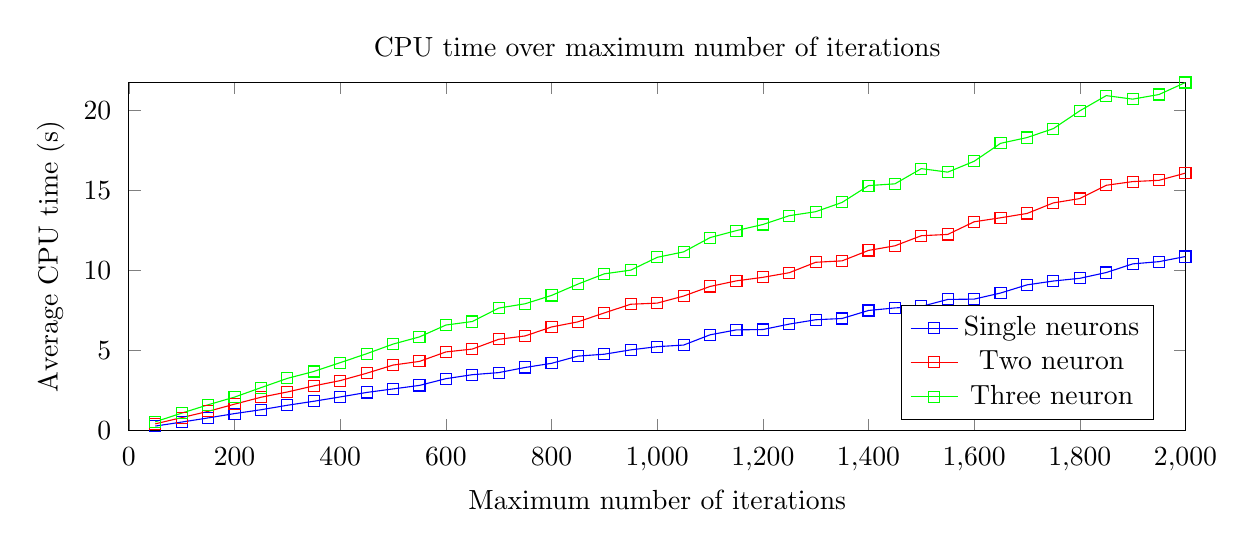
\begin{tikzpicture}
        \begin{axis}[
            width=15cm,
            height=6cm,
            legend pos=south east,
            title={CPU time over maximum number of iterations},
            xlabel={Maximum number of iterations},
            ylabel={Average CPU time (s)},
            xmin=0,
            ymin=0,
            enlargelimits=false,
            xticklabel shift={.1cm},
            yticklabel shift={.1cm} ]
        ]

        \addplot[
            color=blue,
            mark=square,
            ]
            coordinates {
                (50,0.27)(100,0.52)(150,0.78)(200,1.05)(250,1.29)(300,1.57)(350,1.82)(400,2.09)(450,2.37)(500,2.59)(550,2.81)(600,3.23)(650,3.48)(700,3.61)(750,3.93)(800,4.19)(850,4.64)(900,4.76)(950,5.03)(1000,5.23)(1050,5.33)(1100,5.97)(1150,6.28)(1200,6.30)(1250,6.64)(1300,6.91)(1350,6.99)(1400,7.49)(1450,7.65)(1500,7.74)(1550,8.18)(1600,8.20)(1650,8.58)(1700,9.09)(1750,9.33)(1800,9.50)(1850,9.86)(1900,10.40)(1950,10.54)(2000,10.86)
            };
            \addlegendentry{Single neurons}
        \addplot[
            color=red,
            mark=square,
            ]
            coordinates {
                (50,0.41)(100,0.80)(150,1.19)(200,1.64)(250,2.07)(300,2.40)(350,2.78)(400,3.11)(450,3.57)(500,4.08)(550,4.31)(600,4.90)(650,5.08)(700,5.69)(750,5.90)(800,6.46)(850,6.78)(900,7.34)(950,7.88)(1000,7.95)(1050,8.39)(1100,8.99)(1150,9.34)(1200,9.56)(1250,9.85)(1300,10.50)(1350,10.59)(1400,11.24)(1450,11.53)(1500,12.16)(1550,12.24)(1600,13.03)(1650,13.28)(1700,13.55)(1750,14.21)(1800,14.48)(1850,15.31)(1900,15.54)(1950,15.62)(2000,16.07)
            };
            \addlegendentry{Two neuron}
        \addplot[
            color=green,
            mark=square,
            ]
            coordinates {
                (50,0.54)(100,1.08)(150,1.60)(200,2.08)(250,2.67)(300,3.25)(350,3.68)(400,4.23)(450,4.79)(500,5.39)(550,5.84)(600,6.58)(650,6.80)(700,7.64)(750,7.91)(800,8.43)(850,9.14)(900,9.78)(950,10.01)(1000,10.81)(1050,11.15)(1100,12.04)(1150,12.48)(1200,12.86)(1250,13.41)(1300,13.66)(1350,14.24)(1400,15.29)(1450,15.40)(1500,16.35)(1550,16.13)(1600,16.81)(1650,17.93)(1700,18.29)(1750,18.85)(1800,19.96)(1850,20.91)(1900,20.69)(1950,20.98)(2000,21.73)
            };
            \addlegendentry{Three neuron}
        \end{axis}
        \end{tikzpicture}
    \end{center}
    \caption{Performance metrics of the $(1 + 1)$ NA algorithm on the \textit{LocalOpt} benchmark, over different maximum iterations.
    The evolution stopped when the fitness was $2\%$ away from the maximal fitness of $1.0$ or the maximum number of iterations was reached.}
    \label{fig:na_localopt}
\end{figure}

\subsubsection{XOR problem}

The \textit{XOR} problem requires two neurons to be solved. The results of the $(1 + 1)$ NA algorithm on this problem are shown in Table \ref{tab:na_xor}. The evolution stopped
when the fitness was $2\%$ away from the maximal fitness of $1.0$ or the maximum number of $200$ stagnant iterations was reached, and the resolution was set to $400$.
For one neuron, the maximum reachable fitness is $0.75$, while this value corresponds to a local optima in the case of two neurons. A solution and a local optima are shown in Figure \ref{fig:na_xor_visual}.
As it was the case with the \textit{LocalOpt} and \textit{TwoQuarters} benchmarks, even though two neurons are enough to solve the problem, the algorithm often gets stuck in a local optima.
The average fitness is $0.79$ for two neurons, and the number of iterations is $174$, which shows that the algorithm was able to converge to the optimal solution in some cases, but ended up in a local optimla
in most cases.

\begin{figure}
    \centering
    \begin{subfigure}{0.45\textwidth}
        \centering
        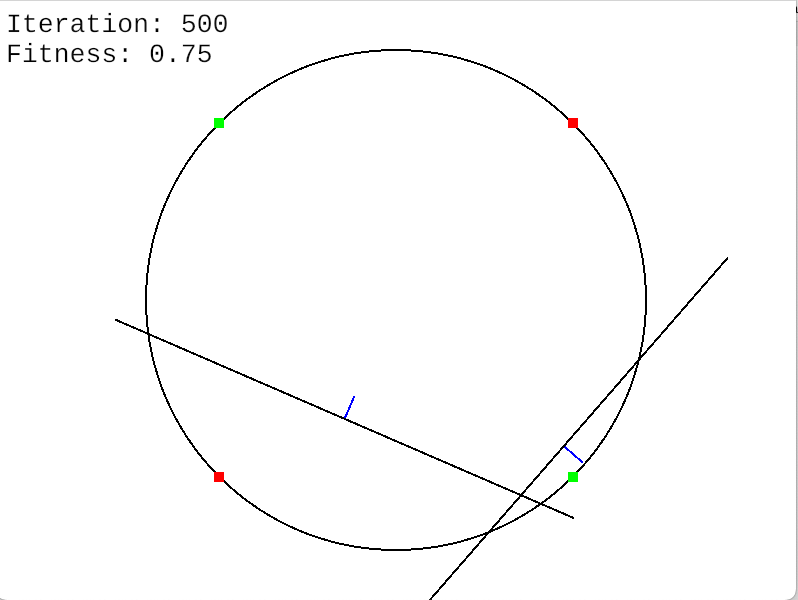
\includegraphics[width=0.9\textwidth]{Pictures/na-xor-localopt}
       \caption{Local optima}
    \end{subfigure}\hfill
    \begin{subfigure}{0.45\textwidth}
        \centering
        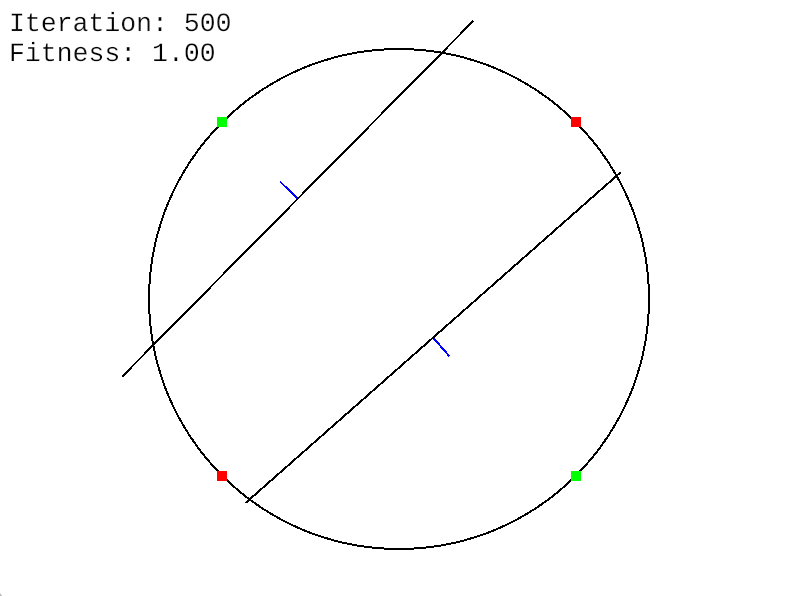
\includegraphics[width=0.9\textwidth]{Pictures/na-xor-opt}
        \caption{Optimal solution}
    \end{subfigure}
    \caption{Visualization of two configurations of the $(1 + 1)$ NA algorithm, with two neurons, after evolution on the \textit{XOR} problem.}
    \label{fig:na_xor_visual}
\end{figure}

\begin{table}
    \caption{Results of the $1 + 1$ NA algorithm on the \textit{XOR} problem. The algorithm was tested with a maximum number of stagnant iterations of $200$.}
    \centering
    \label{tab:na_xor}
    \begin{tabular}{ |c|c|c|c| }
        \hline
        Number of neurons & Average fitness & Average iterations & Average CPU time (s) \\
        \hline
        1 & 0.75 & 200 & 0.01 \\
        \hline
        2 & 0.83 & 168 & 0.01 \\
        \hline\hline
    \end{tabular}
\end{table}

\subsubsection{Proben1 classification problem}

The last problem on which the $(1 + 1)$ NA algorithm was tested is the \textit{Proben1 Cancer1} benchmark. This problem differrs from the previous ones in the sense that the data which
was used to evolve the algorithm is different from the data which was used to evaluate it. In addition, no optimal solution, which would allow us to set the number of neurons, is known in this case,
and the input space is higher-dimensional, as it contains $9$ features. Hence, an interesting experiment consists in testing the algorithm with different number of neurons.
The results are shown in Figure \ref{fig:na_proben1}. Fitness for both the train and test sets is shown.

First of all, it can be seen that the fitness on the train set and test set are very close, which shows that the algorithm did not ovrfit the train set.. In addition, the algorithm performs
best with one neuron, where it reaches an average fitness of $094$ on both sets. However, this is not coherent with the results of the previous experiments, a higher number of neurons should
not result in a decrease in average fitness. This would suggest that the stagnation termination criteria, or at least setting it to a value of $200$, is not well-suited for getting high fitness values
on this problem. One could then try to use a maximum number iteration criteria or set the stagnation criteria to a higher value. Results for the maximum number of iterations set to $10000$ are shown in
\Cref{tab:na_proben1} for one to three neurons. With this high number of maximum iterations, the algorithm was able to reach higher fitness values, which confirms that the stagnation criteria was too low.
However, this value is still too low starting from three neurons. The one neuron case still gets the best result, but more importantly, the CPU time is already way higher than for the other problems.

\begin{table}
    \caption{Results of the $1 + 1$ NA algorithm on the \textit{Proben1 Cancer1} problem. The algorithm was tested with $10000$ iterations.}
    \centering
    \label{tab:na_proben1}
    \begin{tabular}{ |c|c|c|c| }
        \hline
        Number of neurons & Average test fitness & Average CPU time (s) \\
        \hline
        1 & 0.96 & 72 \\
        \hline
        2 & 0.96 & 137 \\
        \hline
        3 & 0.92 & 205 \\
        \hline
        4 & 0.84 & 258 \\
        \hline\hline
    \end{tabular}
\end{table}

\begin{figure}
    \begin{center}
        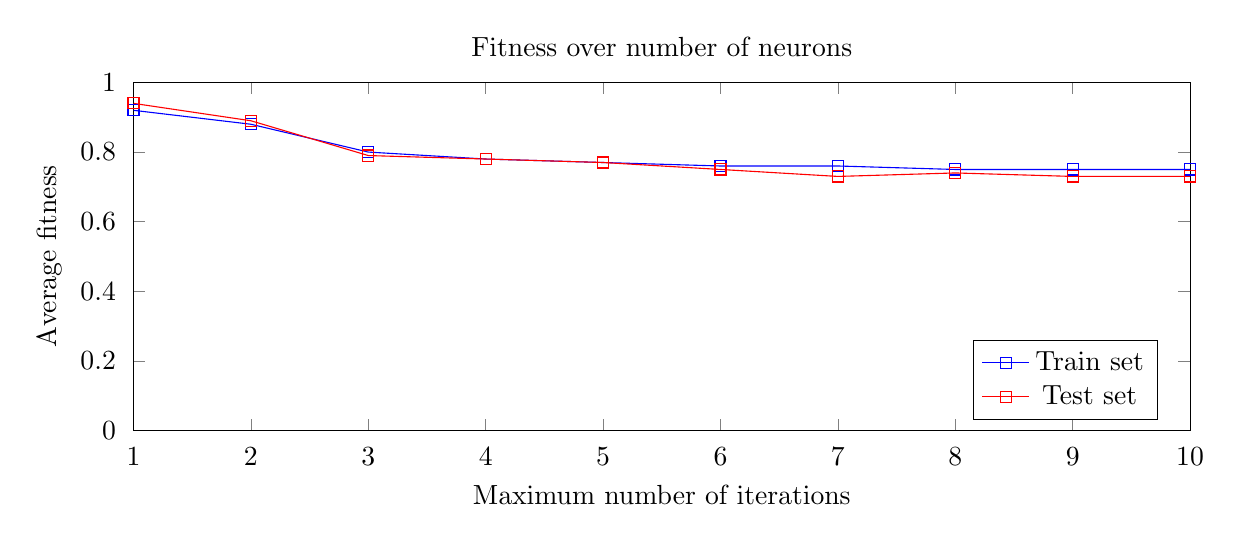
\begin{tikzpicture}
        \begin{axis}[
            width=15cm,
            height=6cm,
            title={Fitness over number of neurons},
            legend pos=south east,
            xlabel={Maximum number of iterations},
            ylabel={Average fitness},
            enlargelimits=false,
            xmin=1,
            ymin=0, ymax=1,
            ytick={0,0.2,...,1},
            xticklabel shift={.1cm},
            yticklabel shift={.1cm} ]
        ]

        \addplot[
            color=blue,
            mark=square,
            ]
            coordinates {
                (1,0.92)(2,0.88)(3,0.80)(4,0.78)(5,0.77)(6,0.76)(7,0.76)(8,0.75)(9,0.75)(10,0.75)
            };
            \addlegendentry{Train set}
        \addplot[
            color=red,
            mark=square,
            ]
            coordinates {
                (1,0.94)(2,0.89)(3,0.79)(4,0.78)(5,0.77)(6,0.75)(7,0.73)(8,0.74)(9,0.73)(10,0.73)
            };
            \addlegendentry{Test set}
        \end{axis}
        \end{tikzpicture}
        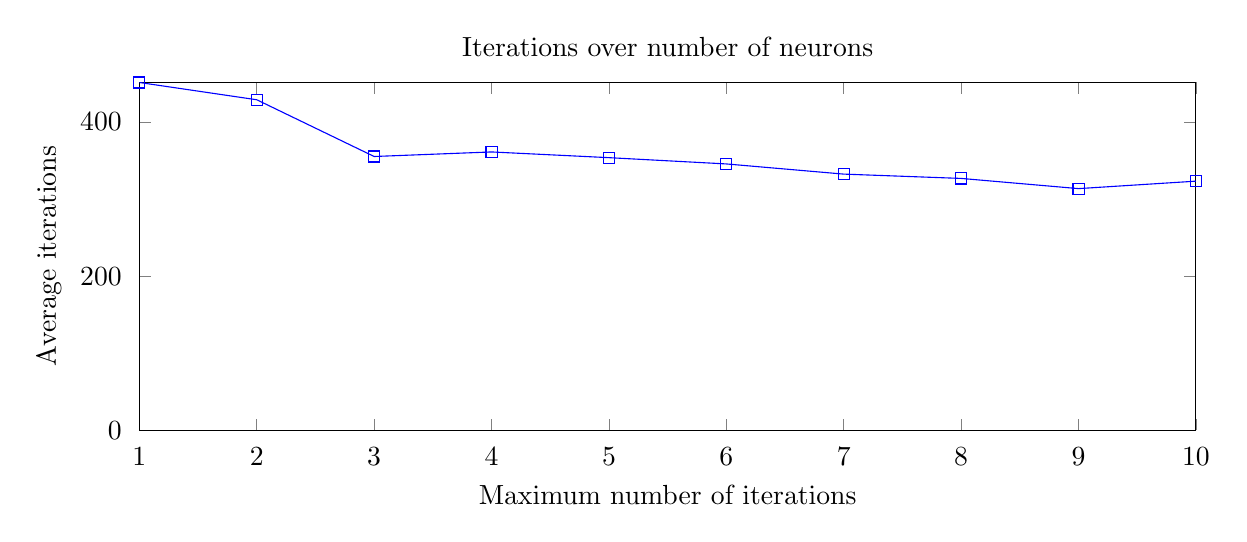
\begin{tikzpicture}
        \begin{axis}[
            width=15cm,
            height=6cm,
            legend pos=south east,
            title={Iterations over number of neurons},
            xlabel={Maximum number of iterations},
            ylabel={Average iterations},
            xmin=1,
            ymin=0,
            enlargelimits=false,
            xticklabel shift={.1cm},
            yticklabel shift={.1cm} ]
        ]

        \addplot[
            color=blue,
            mark=square,
            ]
            coordinates {
                (1,451.20)(2,428.81)(3,355.22)(4,361.13)(5,353.71)(6,345.58)(7,332.38)(8,326.79)(9,313.57)(10,323.24)
            };
        \end{axis}
        \end{tikzpicture}
        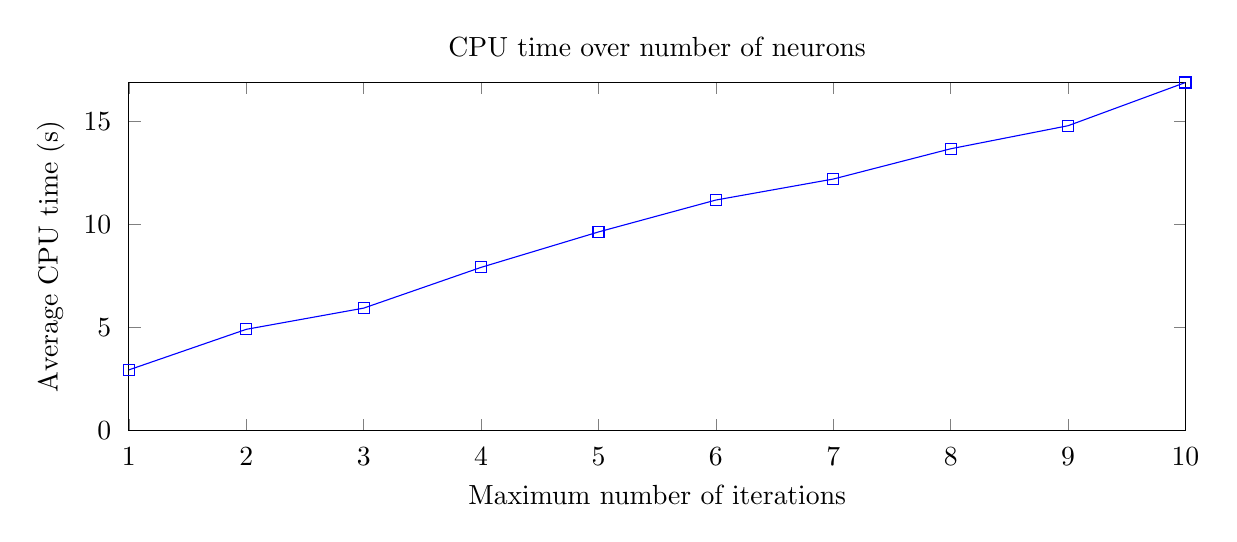
\begin{tikzpicture}
        \begin{axis}[
            width=15cm,
            height=6cm,
            legend pos=south east,
            title={CPU time over number of neurons},
            xlabel={Maximum number of iterations},
            ylabel={Average CPU time (s)},
            xmin=1,
            ymin=0,
            enlargelimits=false,
            xticklabel shift={.1cm},
            yticklabel shift={.1cm} ]
        ]

        \addplot[
            color=blue,
            mark=square,
            ]
            coordinates {
                (1,2.94)(2,4.91)(3,5.94)(4,7.92)(5,9.64)(6,11.19)(7,12.21)(8,13.68)(9,14.80)(10,16.90)
            };
        \end{axis}
        \end{tikzpicture}
    \end{center}
    \caption{Performance metrics of the $(1 + 1)$ NA algorithm on the \textit{Proben1 Cancer1} benchmark, over different number of neurons.
    The evolution stopped when the fitness was $2\%$ away from the maximal fitness of $1.0$ or the maximum number of $200$ stagnant iterations was reached.}
    \label{fig:na_proben1}
\end{figure}

\subsection{Results of the BNA algorithm}

The BNA algorithm can be applied to binary classification problems. As it is the case for the $(1 + 1)$ NA algorithm, the BNA algorithm was tested on the spere classification problems,
the \textit{XOR} problem and the \textit{Cancer1} classification problem. The parameters which can be tuned for this algorithm are the resolution and the number of V-neurons,
Varying the resolution would simply highlight the same properties as the ones observed for the $(1 + 1)$ NA algorithm. Thus the focus will be on the number of V-neurons and the the termination
criteria for the algorithm. For the following experiments, the resolution was set to $400$.

\subsubsection{Unit-sphere classification problems}

The first experiment consisted in testing the algorithm on the \textit{Half} and \textit{Quarter} benchmarks. The results are shown in Figure \ref{fig:bna_half_quarter}. The algorithm
was tested with a maximum number of iterations ranging from $5$ to $300$. The evolution stopped when the fitness was $2\%$ away from the maximal fitness of $1.0$ or the maximum number
of iterations was reached. For both problems, it can be seen that the fitness converges to $1.0$ and the number of iterations taken by the algorithm plateaus around $110$ iterations. Furthermore,
as it was the case for the $(1 + 1)$ NA algorithm, the results on the two problems were almost identical, and the CPU time graphs reflect how the CPU time is proportional to the number of iterations.

\begin{figure}
    \begin{center}
        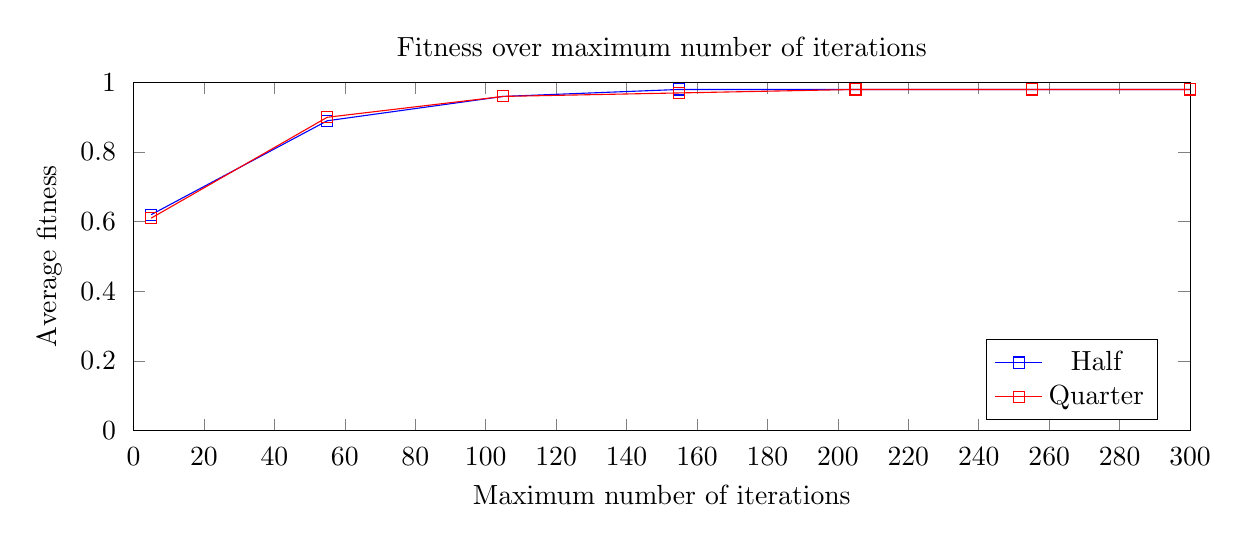
\begin{tikzpicture}
        \begin{axis}[
            width=15cm,
            height=6cm,
            title={Fitness over maximum number of iterations},
            legend pos=south east,
            xlabel={Maximum number of iterations},
            ylabel={Average fitness},
            enlargelimits=false,
            xmin=0,
            ymin=0, ymax=1,
            ytick={0,0.2,...,1},
            xticklabel shift={.1cm},
            yticklabel shift={.1cm} ]
        ]

        \addplot[
            color=blue,
            mark=square,
            ]
            coordinates {
                (5,0.62)(55,0.89)(105,0.96)(155,0.98)(205,0.98)(255,0.98)(300,0.98)
            };
            \addlegendentry{Half}
        \addplot[
            color=red,
            mark=square,
            ]
            coordinates {
                (5,0.61)(55,0.90)(105,0.96)(155,0.97)(205,0.98)(255,0.98)(300,0.98)
            };
            \addlegendentry{Quarter}
        \end{axis}
        \end{tikzpicture}
        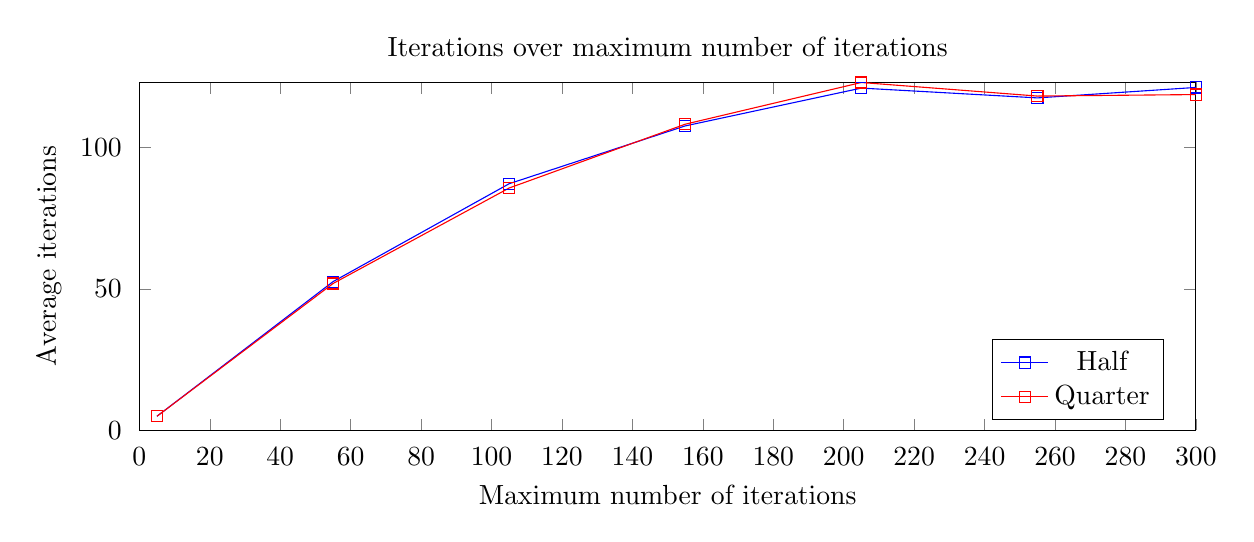
\begin{tikzpicture}
        \begin{axis}[
            width=15cm,
            height=6cm,
            legend pos=south east,
            title={Iterations over maximum number of iterations},
            xlabel={Maximum number of iterations},
            ylabel={Average iterations},
            xmin=0,
            ymin=0,
            enlargelimits=false,
            xticklabel shift={.1cm},
            yticklabel shift={.1cm} ]
        ]

        \addplot[
            color=blue,
            mark=square,
            ]
            coordinates {
                (5,5.00)(55,52.63)(105,87.26)(155,107.71)(205,121.09)(255,117.62)(300,121.32)
            };
            \addlegendentry{Half}
        \addplot[
            color=red,
            mark=square,
            ]
            coordinates {
                (5,5.00)(55,51.96)(105,85.74)(155,108.32)(205,123.07)(255,118.27)(300,118.80)
            };
            \addlegendentry{Quarter}
        \end{axis}
        \end{tikzpicture}
        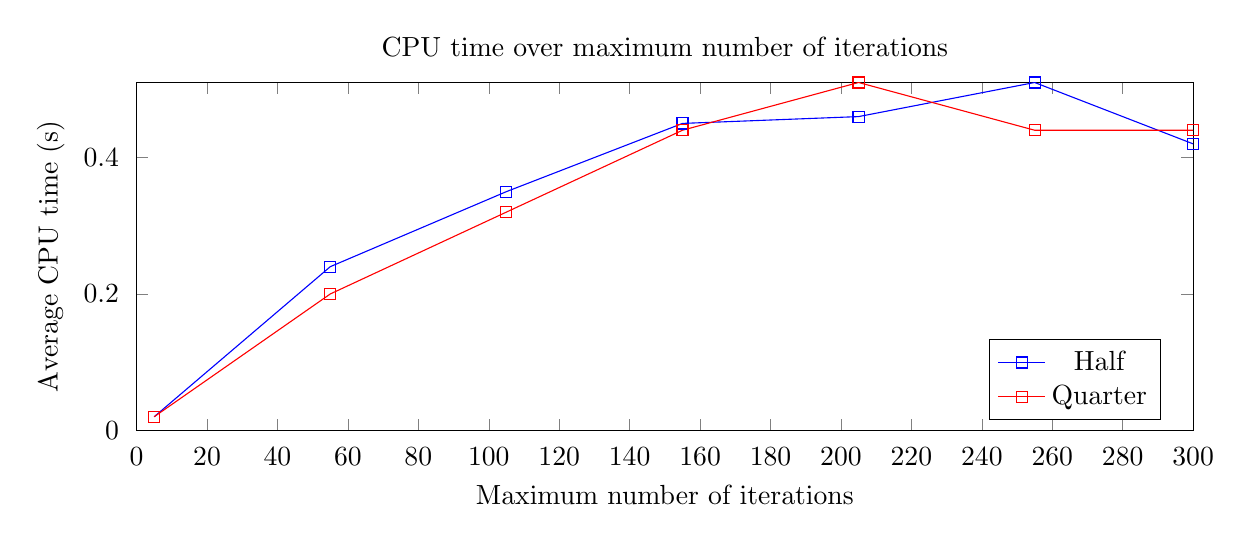
\begin{tikzpicture}
        \begin{axis}[
            width=15cm,
            height=6cm,
            legend pos=south east,
            title={CPU time over maximum number of iterations},
            xlabel={Maximum number of iterations},
            ylabel={Average CPU time (s)},
            xmin=0,
            ymin=0,
            enlargelimits=false,
            xticklabel shift={.1cm},
            yticklabel shift={.1cm} ]
        ]

        \addplot[
            color=blue,
            mark=square,
            ]
            coordinates {
                (5,0.02)(55,0.24)(105,0.35)(155,0.45)(205,0.46)(255,0.51)(300,0.42)
            };
            \addlegendentry{Half}
        \addplot[
            color=red,
            mark=square,
            ]
            coordinates {
                (5,0.02)(55,0.20)(105,0.32)(155,0.44)(205,0.51)(255,0.44)(300,0.44)
            };
            \addlegendentry{Quarter}
        \end{axis}
        \end{tikzpicture}
    \end{center}
    \caption{Performance metrics of the BNA algorithm on the \textit{Half} and \textit{Quarter} benchmarks, over different maximum iterations.
    The evolution stopped when the fitness was $2\%$ away from the maximal fitness of $1.0$ or the maximum number of iterations was reached.}
    \label{fig:bna_half_quarter}
\end{figure}

The results for the \textit{TwoQuarters} benchmark are shown in \Cref{fig:bna_twoquarters} and the results for the \textit{LocalOpt} benchmark are shown in \Cref{fig:bna_localopt}.
For both problems, the same observations can be made as for the $(1 + 1)$ NA algorithm. For the \textit{TwoQuarters} benchmark, with two V-neurons, the fitness converges to approximately $0.85$,
while the algorithm quickly reaches the maximal fitness of $0.75$ in the case of one V-neuron. Regarding the \texit{LocalOpt} benchmark, it was able to find the optimal solution once and also
got stcuk in local optima, with an average fitness converging to $0.75$ for all three cases. Examples of local optima and optimal solutions are shown in \Cref{fig:bna_twoquarters_visual}
and \Cref{fig:bna_localopt_visual}.

\begin{figure}
    \centering
    \begin{subfigure}{0.45\textwidth}
        \centering
        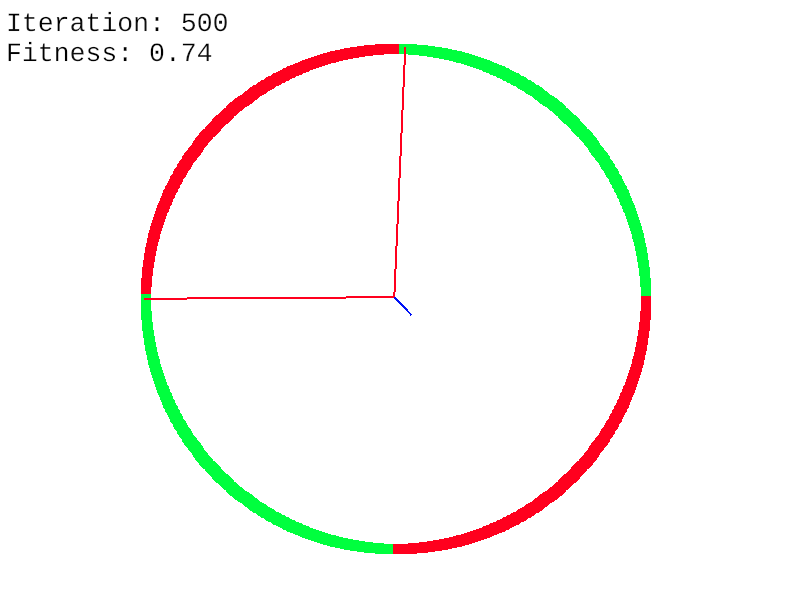
\includegraphics[width=0.9\textwidth]{Pictures/bna-twoquarters-localopt}
       \caption{Local optima}
    \end{subfigure}\hfill
    \begin{subfigure}{0.45\textwidth}
        \centering
        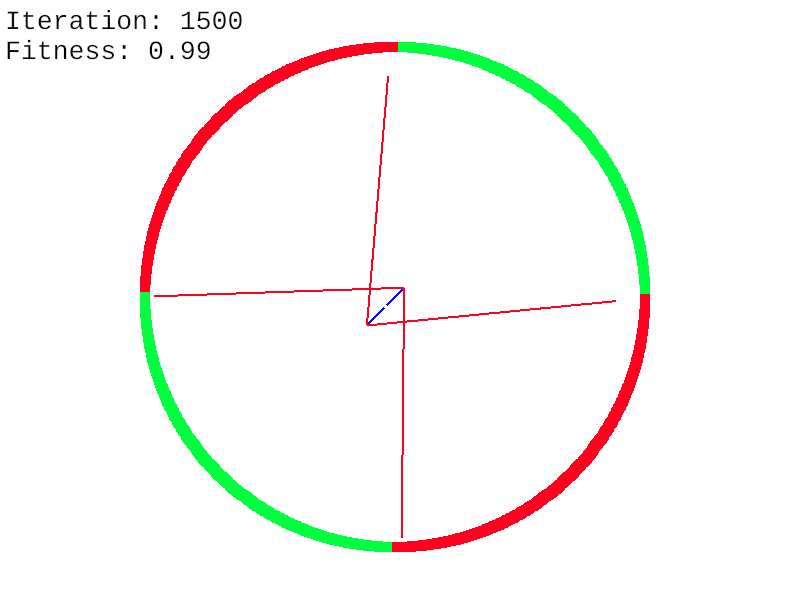
\includegraphics[width=0.9\textwidth]{Pictures/bna-twoquarters-opt}
        \caption{Optimal solution}
    \end{subfigure}
    \caption{Visualization of two configurations of the BNA algorithm, with two V-neurons, after evolution on the \textit{TwoQuarters} problem.}
    \label{fig:bna_twoquarters_visual}
\end{figure}

\begin{figure}
    \centering
    \begin{subfigure}{0.3\textwidth}
        \centering
        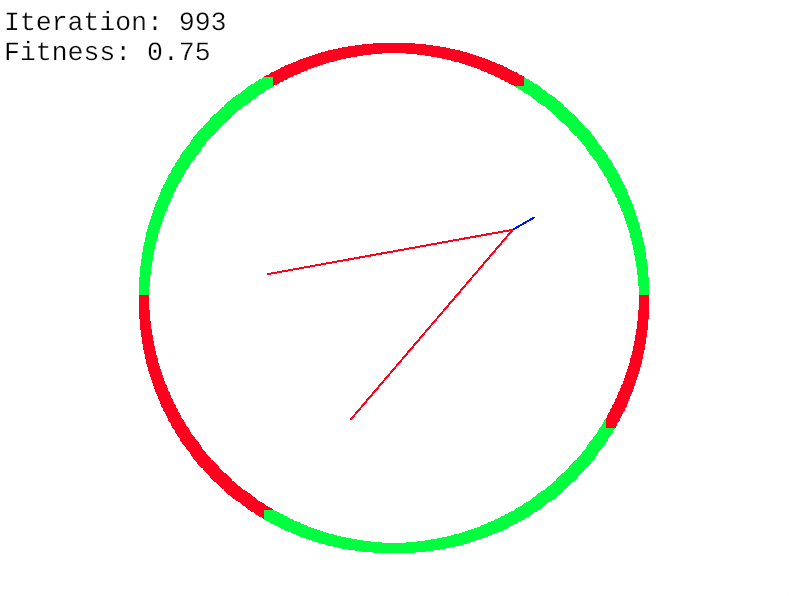
\includegraphics[width=0.9\textwidth]{Pictures/bna-localopt-75}
       \caption{Local optima.}
    \end{subfigure}\hfill
    \begin{subfigure}{0.3\textwidth}
        \centering
        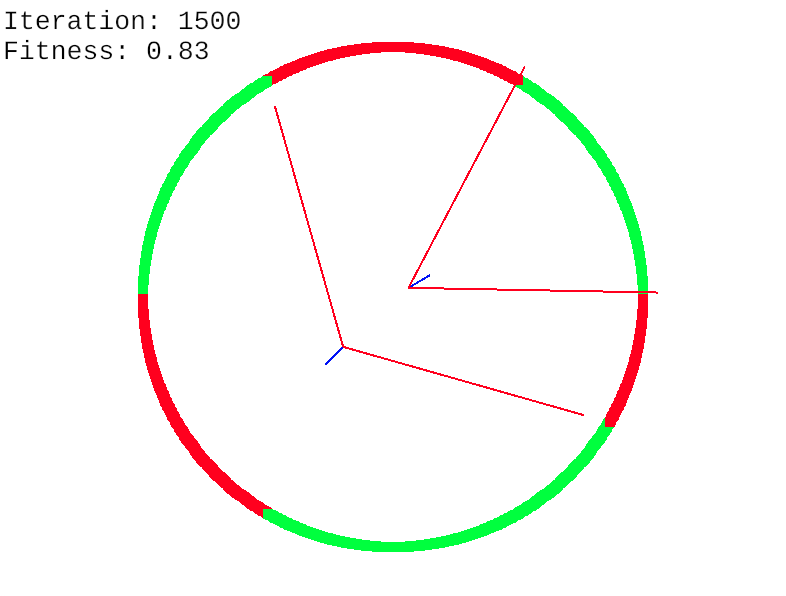
\includegraphics[width=0.9\textwidth]{Pictures/bna-localopt-83}
        \caption{Local optima.}
    \end{subfigure}\hfill
    \begin{subfigure}{0.3\textwidth}
        \centering
        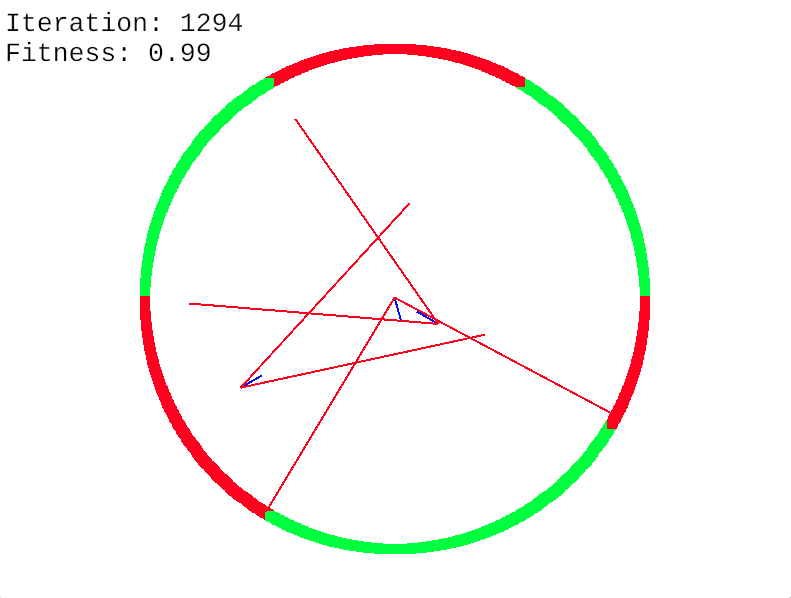
\includegraphics[width=0.9\textwidth]{Pictures/bna-localopt-1}
        \caption{Optimal solution.}
    \end{subfigure}
    \caption{Visualization of two configurations of the BNA algorithm, with three V-neurons, after evolution on the \textit{LocalOpt} problem.}
    \label{fig:bna_localopt_visual}
\end{figure}

\begin{figure}
    \begin{center}
        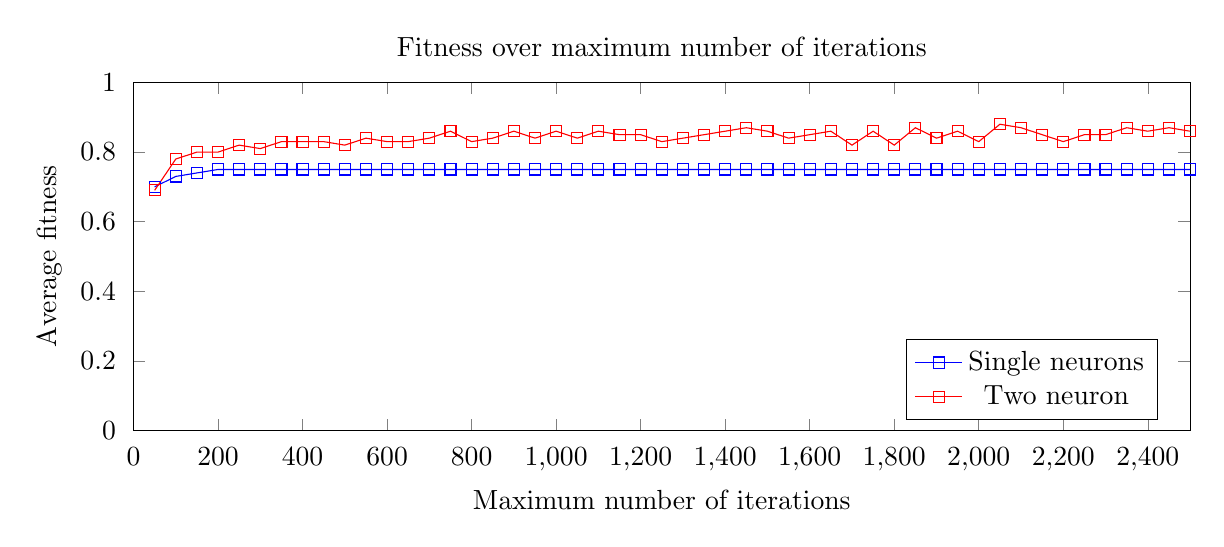
\begin{tikzpicture}
        \begin{axis}[
            width=15cm,
            height=6cm,
            title={Fitness over maximum number of iterations},
            legend pos=south east,
            xlabel={Maximum number of iterations},
            ylabel={Average fitness},
            enlargelimits=false,
            xmin=0,
            ymin=0, ymax=1,
            ytick={0,0.2,...,1},
            xticklabel shift={.1cm},
            yticklabel shift={.1cm} ]
        ]

        \addplot[
            color=blue,
            mark=square,
            ]
            coordinates {
(50,0.70)(100,0.73)(150,0.74)(200,0.75)(250,0.75)(300,0.75)(350,0.75)(400,0.75)(450,0.75)(500,0.75)(550,0.75)(600,0.75)(650,0.75)(700,0.75)(750,0.75)(800,0.75)(850,0.75)(900,0.75)(950,0.75)(1000,0.75)(1050,0.75)(1100,0.75)(1150,0.75)(1200,0.75)(1250,0.75)(1300,0.75)(1350,0.75)(1400,0.75)(1450,0.75)(1500,0.75)(1550,0.75)(1600,0.75)(1650,0.75)(1700,0.75)(1750,0.75)(1800,0.75)(1850,0.75)(1900,0.75)(1950,0.75)(2000,0.75)(2050,0.75)(2100,0.75)(2150,0.75)(2200,0.75)(2250,0.75)(2300,0.75)(2350,0.75)(2400,0.75)(2450,0.75)(2500,0.75)
            };
            \addlegendentry{Single neurons}
        \addplot[
            color=red,
            mark=square,
            ]
            coordinates {
(50,0.69)(100,0.78)(150,0.80)(200,0.80)(250,0.82)(300,0.81)(350,0.83)(400,0.83)(450,0.83)(500,0.82)(550,0.84)(600,0.83)(650,0.83)(700,0.84)(750,0.86)(800,0.83)(850,0.84)(900,0.86)(950,0.84)(1000,0.86)(1050,0.84)(1100,0.86)(1150,0.85)(1200,0.85)(1250,0.83)(1300,0.84)(1350,0.85)(1400,0.86)(1450,0.87)(1500,0.86)(1550,0.84)(1600,0.85)(1650,0.86)(1700,0.82)(1750,0.86)(1800,0.82)(1850,0.87)(1900,0.84)(1950,0.86)(2000,0.83)(2050,0.88)(2100,0.87)(2150,0.85)(2200,0.83)(2250,0.85)(2300,0.85)(2350,0.87)(2400,0.86)(2450,0.87)(2500,0.86)
            };
            \addlegendentry{Two neuron}
        \end{axis}
        \end{tikzpicture}
        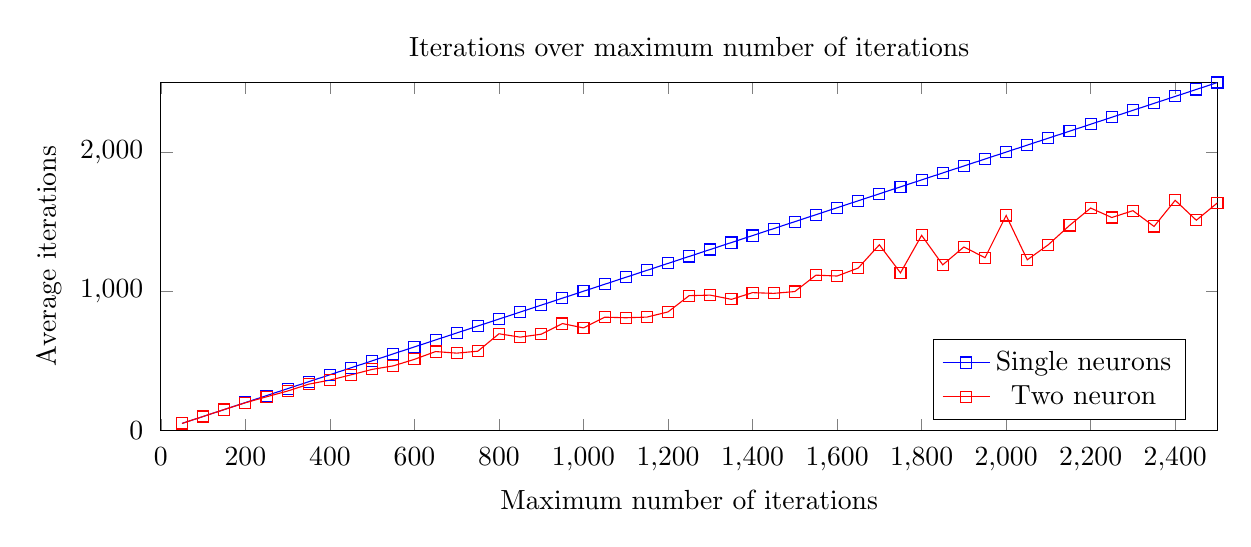
\begin{tikzpicture}
        \begin{axis}[
            width=15cm,
            height=6cm,
            legend pos=south east,
            title={Iterations over maximum number of iterations},
            xlabel={Maximum number of iterations},
            ylabel={Average iterations},
            xmin=0,
            ymin=0,
            enlargelimits=false,
            xticklabel shift={.1cm},
            yticklabel shift={.1cm} ]
        ]

        \addplot[
            color=blue,
            mark=square,
            ]
            coordinates {
(50,50.00)(100,100.00)(150,150.00)(200,200.00)(250,250.00)(300,300.00)(350,350.00)(400,400.00)(450,450.00)(500,500.00)(550,550.00)(600,600.00)(650,650.00)(700,700.00)(750,750.00)(800,800.00)(850,850.00)(900,900.00)(950,950.00)(1000,1000.00)(1050,1050.00)(1100,1100.00)(1150,1150.00)(1200,1200.00)(1250,1250.00)(1300,1300.00)(1350,1350.00)(1400,1400.00)(1450,1450.00)(1500,1500.00)(1550,1550.00)(1600,1600.00)(1650,1650.00)(1700,1700.00)(1750,1750.00)(1800,1800.00)(1850,1850.00)(1900,1900.00)(1950,1950.00)(2000,2000.00)(2050,2050.00)(2100,2100.00)(2150,2150.00)(2200,2200.00)(2250,2250.00)(2300,2300.00)(2350,2350.00)(2400,2400.00)(2450,2450.00)(2500,2500.00)
            };
            \addlegendentry{Single neurons}
        \addplot[
            color=red,
            mark=square,
            ]
            coordinates {
(50,50.00)(100,99.92)(150,150.00)(200,198.51)(250,241.50)(300,282.96)(350,332.40)(400,361.51)(450,399.29)(500,438.45)(550,463.70)(600,510.75)(650,566.58)(700,555.12)(750,569.20)(800,694.31)(850,670.17)(900,691.26)(950,767.70)(1000,736.54)(1050,813.48)(1100,809.46)(1150,814.14)(1200,851.38)(1250,968.46)(1300,972.02)(1350,941.72)(1400,989.87)(1450,984.70)(1500,997.75)(1550,1115.48)(1600,1109.32)(1650,1166.71)(1700,1333.93)(1750,1132.14)(1800,1401.49)(1850,1189.76)(1900,1318.19)(1950,1240.79)(2000,1544.52)(2050,1225.65)(2100,1334.69)(2150,1472.85)(2200,1597.69)(2250,1529.85)(2300,1578.75)(2350,1465.73)(2400,1653.33)(2450,1510.16)(2500,1635.20)
            };
            \addlegendentry{Two neuron}
        \end{axis}
        \end{tikzpicture}
        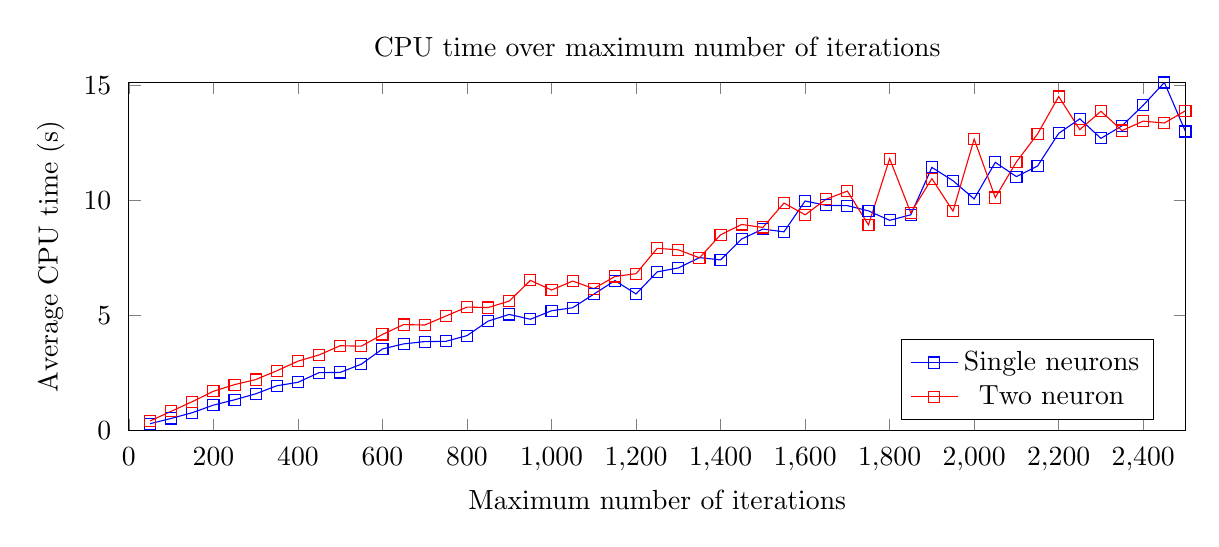
\begin{tikzpicture}
        \begin{axis}[
            width=15cm,
            height=6cm,
            legend pos=south east,
            title={CPU time over maximum number of iterations},
            xlabel={Maximum number of iterations},
            ylabel={Average CPU time (s)},
            xmin=0,
            ymin=0,
            enlargelimits=false,
            xticklabel shift={.1cm},
            yticklabel shift={.1cm} ]
        ]

        \addplot[
            color=blue,
            mark=square,
            ]
            coordinates {
(50,0.29)(100,0.52)(150,0.77)(200,1.10)(250,1.33)(300,1.59)(350,1.94)(400,2.09)(450,2.51)(500,2.52)(550,2.88)(600,3.54)(650,3.76)(700,3.86)(750,3.87)(800,4.12)(850,4.75)(900,5.04)(950,4.83)(1000,5.20)(1050,5.33)(1100,5.92)(1150,6.51)(1200,5.93)(1250,6.89)(1300,7.06)(1350,7.51)(1400,7.41)(1450,8.32)(1500,8.75)(1550,8.63)(1600,9.97)(1650,9.78)(1700,9.77)(1750,9.54)(1800,9.13)(1850,9.37)(1900,11.43)(1950,10.85)(2000,10.06)(2050,11.65)(2100,11.03)(2150,11.49)(2200,12.91)(2250,13.54)(2300,12.69)(2350,13.24)(2400,14.13)(2450,15.12)(2500,12.99)
            };
            \addlegendentry{Single neurons}
        \addplot[
            color=red,
            mark=square,
            ]
            coordinates {
(50,0.41)(100,0.83)(150,1.25)(200,1.70)(250,1.99)(300,2.21)(350,2.59)(400,3.01)(450,3.28)(500,3.68)(550,3.66)(600,4.17)(650,4.60)(700,4.58)(750,4.97)(800,5.36)(850,5.34)(900,5.62)(950,6.52)(1000,6.10)(1050,6.49)(1100,6.16)(1150,6.69)(1200,6.81)(1250,7.91)(1300,7.85)(1350,7.50)(1400,8.50)(1450,8.95)(1500,8.82)(1550,9.88)(1600,9.37)(1650,10.05)(1700,10.40)(1750,8.93)(1800,11.81)(1850,9.46)(1900,10.94)(1950,9.53)(2000,12.66)(2050,10.12)(2100,11.67)(2150,12.88)(2200,14.51)(2250,13.07)(2300,13.87)(2350,13.03)(2400,13.44)(2450,13.36)(2500,13.89)
            };
            \addlegendentry{Two neuron}
        \end{axis}
        \end{tikzpicture}
    \end{center}
    \caption{Performance metrics of the BNA algorithm on the \textit{TwoQuarters} benchmark, over different maximum iterations.
    The evolution stopped when the fitness was $2\%$ away from the maximal fitness of $1.0$ or the maximum number of iterations was reached.}
    \label{fig:bna_twoquarters}
\end{figure}

\begin{figure}
    \begin{center}
        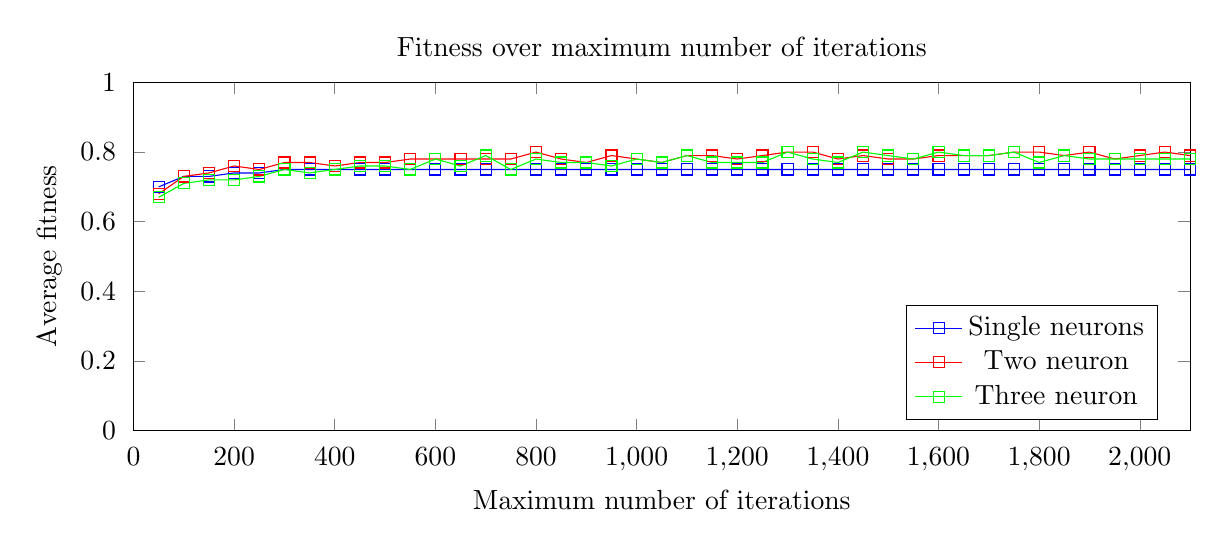
\begin{tikzpicture}
        \begin{axis}[
            width=15cm,
            height=6cm,
            title={Fitness over maximum number of iterations},
            legend pos=south east,
            xlabel={Maximum number of iterations},
            ylabel={Average fitness},
            enlargelimits=false,
            xmin=0,
            ymin=0, ymax=1,
            ytick={0,0.2,...,1},
            xticklabel shift={.1cm},
            yticklabel shift={.1cm} ]
        ]

        \addplot[
            color=blue,
            mark=square,
            ]
            coordinates {
                (50,0.70)(100,0.73)(150,0.73)(200,0.74)(250,0.74)(300,0.75)(350,0.75)(400,0.75)(450,0.75)(500,0.75)(550,0.75)(600,0.75)(650,0.75)(700,0.75)(750,0.75)(800,0.75)(850,0.75)(900,0.75)(950,0.75)(1000,0.75)(1050,0.75)(1100,0.75)(1150,0.75)(1200,0.75)(1250,0.75)(1300,0.75)(1350,0.75)(1400,0.75)(1450,0.75)(1500,0.75)(1550,0.75)(1600,0.75)(1650,0.75)(1700,0.75)(1750,0.75)(1800,0.75)(1850,0.75)(1900,0.75)(1950,0.75)(2000,0.75)(2050,0.75)(2100,0.75)
            };
            \addlegendentry{Single neurons}
        \addplot[
            color=red,
            mark=square,
            ]
            coordinates {
                (50,0.68)(100,0.73)(150,0.74)(200,0.76)(250,0.75)(300,0.77)(350,0.77)(400,0.76)(450,0.77)(500,0.77)(550,0.78)(600,0.78)(650,0.78)(700,0.78)(750,0.78)(800,0.80)(850,0.78)(900,0.77)(950,0.79)(1000,0.78)(1050,0.77)(1100,0.79)(1150,0.79)(1200,0.78)(1250,0.79)(1300,0.80)(1350,0.80)(1400,0.78)(1450,0.79)(1500,0.78)(1550,0.78)(1600,0.79)(1650,0.79)(1700,0.79)(1750,0.80)(1800,0.80)(1850,0.79)(1900,0.80)(1950,0.78)(2000,0.79)(2050,0.80)(2100,0.79)
            };
            \addlegendentry{Two neuron}
        \addplot[
            color=green,
            mark=square,
            ]
            coordinates {
                (50,0.67)(100,0.71)(150,0.72)(200,0.72)(250,0.73)(300,0.75)(350,0.74)(400,0.75)(450,0.76)(500,0.76)(550,0.75)(600,0.78)(650,0.76)(700,0.79)(750,0.75)(800,0.78)(850,0.77)(900,0.77)(950,0.76)(1000,0.78)(1050,0.77)(1100,0.79)(1150,0.77)(1200,0.77)(1250,0.77)(1300,0.80)(1350,0.78)(1400,0.77)(1450,0.80)(1500,0.79)(1550,0.78)(1600,0.80)(1650,0.79)(1700,0.79)(1750,0.80)(1800,0.77)(1850,0.79)(1900,0.78)(1950,0.78)(2000,0.78)(2050,0.78)(2100,0.78)
            };
            \addlegendentry{Three neuron}
        \end{axis}
        \end{tikzpicture}
        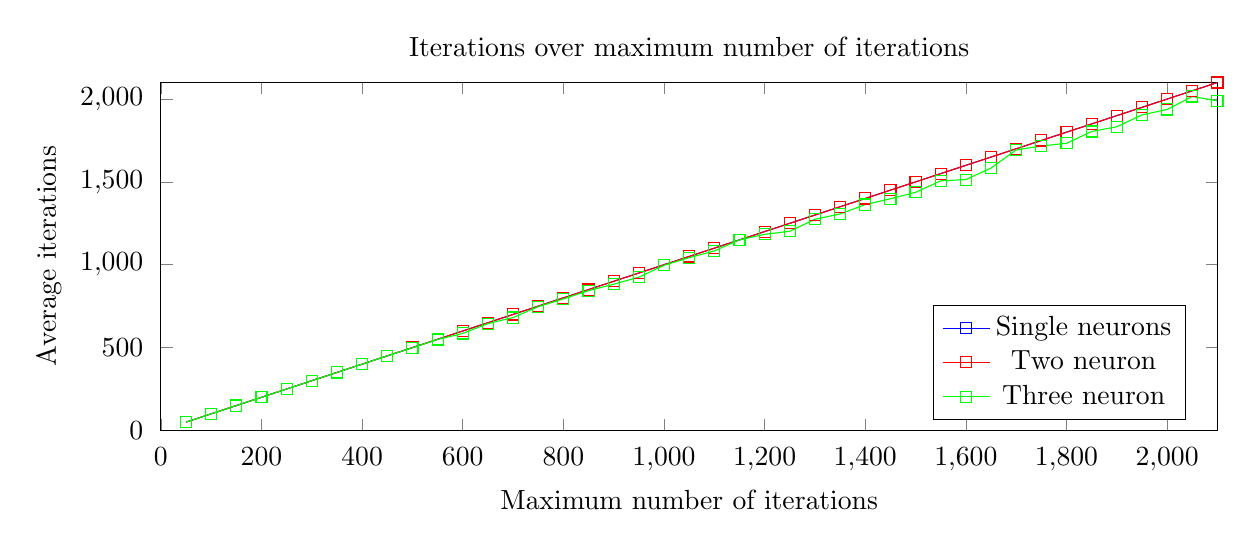
\begin{tikzpicture}
        \begin{axis}[
            width=15cm,
            height=6cm,
            legend pos=south east,
            title={Iterations over maximum number of iterations},
            xlabel={Maximum number of iterations},
            ylabel={Average iterations},
            xmin=0,
            ymin=0,
            enlargelimits=false,
            xticklabel shift={.1cm},
            yticklabel shift={.1cm} ]
        ]

        \addplot[
            color=blue,
            mark=square,
            ]
            coordinates {
                (50,50.00)(100,100.00)(150,150.00)(200,200.00)(250,250.00)(300,300.00)(350,350.00)(400,400.00)(450,450.00)(500,500.00)(550,550.00)(600,600.00)(650,650.00)(700,700.00)(750,750.00)(800,800.00)(850,850.00)(900,900.00)(950,950.00)(1000,1000.00)(1050,1050.00)(1100,1100.00)(1150,1150.00)(1200,1200.00)(1250,1250.00)(1300,1300.00)(1350,1350.00)(1400,1400.00)(1450,1450.00)(1500,1500.00)(1550,1550.00)(1600,1600.00)(1650,1650.00)(1700,1700.00)(1750,1750.00)(1800,1800.00)(1850,1850.00)(1900,1900.00)(1950,1950.00)(2000,2000.00)(2050,2050.00)(2100,2100.00)
            };
            \addlegendentry{Single neurons}
        \addplot[
            color=red,
            mark=square,
            ]
            coordinates {
                (50,50.00)(100,100.00)(150,150.00)(200,200.00)(250,250.00)(300,300.00)(350,350.00)(400,400.00)(450,450.00)(500,500.00)(550,550.00)(600,600.00)(650,650.00)(700,700.00)(750,750.00)(800,800.00)(850,850.00)(900,900.00)(950,950.00)(1000,1000.00)(1050,1050.00)(1100,1100.00)(1150,1150.00)(1200,1200.00)(1250,1250.00)(1300,1300.00)(1350,1350.00)(1400,1400.00)(1450,1450.00)(1500,1500.00)(1550,1550.00)(1600,1600.00)(1650,1650.00)(1700,1700.00)(1750,1750.00)(1800,1800.00)(1850,1850.00)(1900,1900.00)(1950,1950.00)(2000,2000.00)(2050,2050.00)(2100,2100.00)
            };
            \addlegendentry{Two neuron}
        \addplot[
            color=green,
            mark=square,
            ]
            coordinates {
                (50,50.00)(100,100.00)(150,150.00)(200,200.00)(250,250.00)(300,300.00)(350,350.00)(400,400.00)(450,450.00)(500,498.69)(550,548.75)(600,585.31)(650,644.70)(700,681.21)(750,746.81)(800,793.97)(850,843.65)(900,882.82)(950,924.71)(1000,996.55)(1050,1042.52)(1100,1083.37)(1150,1150.00)(1200,1183.52)(1250,1202.19)(1300,1274.40)(1350,1306.74)(1400,1363.23)(1450,1397.99)(1500,1437.08)(1550,1506.49)(1600,1513.89)(1650,1583.68)(1700,1693.09)(1750,1716.86)(1800,1732.89)(1850,1804.30)(1900,1832.85)(1950,1904.38)(2000,1937.28)(2050,2015.75)(2100,1988.72)
            };
            \addlegendentry{Three neuron}
        \end{axis}
        \end{tikzpicture}
        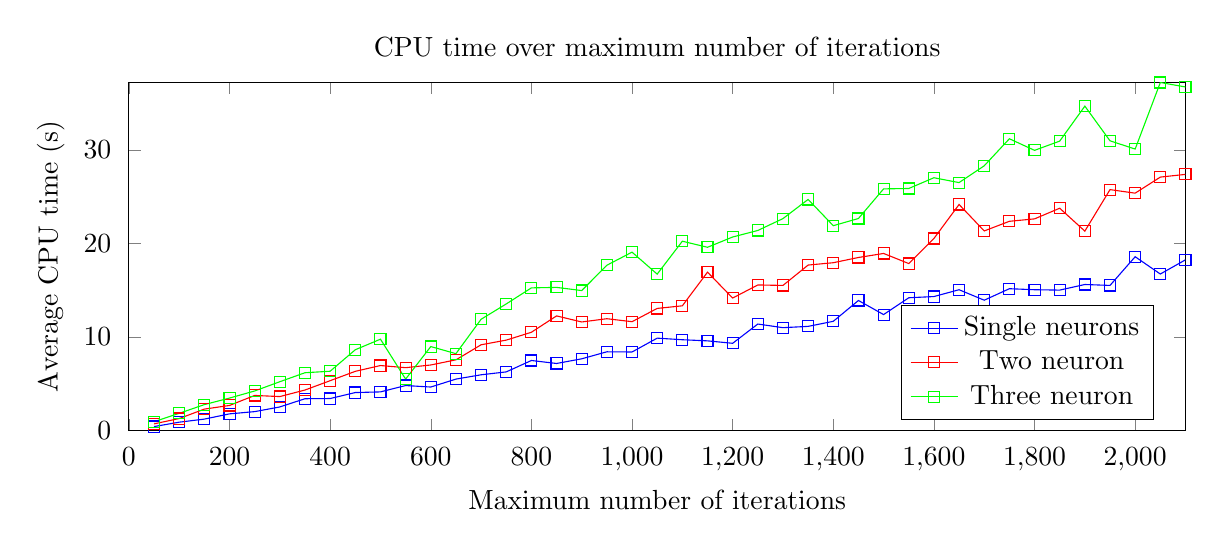
\begin{tikzpicture}
        \begin{axis}[
            width=15cm,
            height=6cm,
            legend pos=south east,
            title={CPU time over maximum number of iterations},
            xlabel={Maximum number of iterations},
            ylabel={Average CPU time (s)},
            xmin=0,
            ymin=0,
            enlargelimits=false,
            xticklabel shift={.1cm},
            yticklabel shift={.1cm} ]
        ]

        \addplot[
            color=blue,
            mark=square,
            ]
            coordinates {
                (50,0.41)(100,0.88)(150,1.21)(200,1.77)(250,2.01)(300,2.51)(350,3.39)(400,3.41)(450,4.05)(500,4.12)(550,4.80)(600,4.64)(650,5.49)(700,5.95)(750,6.26)(800,7.48)(850,7.16)(900,7.66)(950,8.41)(1000,8.39)(1050,9.87)(1100,9.70)(1150,9.58)(1200,9.32)(1250,11.38)(1300,10.99)(1350,11.13)(1400,11.67)(1450,13.90)(1500,12.39)(1550,14.19)(1600,14.32)(1650,15.05)(1700,13.93)(1750,15.16)(1800,15.05)(1850,15.01)(1900,15.61)(1950,15.51)(2000,18.58)(2050,16.73)(2100,18.25)
            };
            \addlegendentry{Single neurons}
        \addplot[
            color=red,
            mark=square,
            ]
            coordinates {
                (50,0.70)(100,1.27)(150,2.28)(200,2.67)(250,3.74)(300,3.62)(350,4.32)(400,5.32)(450,6.32)(500,6.94)(550,6.71)(600,7.00)(650,7.55)(700,9.16)(750,9.66)(800,10.50)(850,12.25)(900,11.60)(950,11.95)(1000,11.63)(1050,13.05)(1100,13.33)(1150,16.93)(1200,14.16)(1250,15.56)(1300,15.51)(1350,17.69)(1400,17.94)(1450,18.50)(1500,18.93)(1550,17.85)(1600,20.53)(1650,24.17)(1700,21.34)(1750,22.37)(1800,22.63)(1850,23.77)(1900,21.32)(1950,25.76)(2000,25.38)(2050,27.10)(2100,27.39)
            };
            \addlegendentry{Two neuron}
        \addplot[
            color=green,
            mark=square,
            ]
            coordinates {
                (50,0.93)(100,1.83)(150,2.76)(200,3.46)(250,4.22)(300,5.21)(350,6.17)(400,6.33)(450,8.63)(500,9.76)(550,5.49)(600,8.97)(650,8.21)(700,11.89)(750,13.53)(800,15.25)(850,15.30)(900,14.96)(950,17.67)(1000,19.07)(1050,16.72)(1100,20.24)(1150,19.59)(1200,20.69)(1250,21.39)(1300,22.66)(1350,24.71)(1400,21.90)(1450,22.67)(1500,25.84)(1550,25.88)(1600,27.03)(1650,26.51)(1700,28.31)(1750,31.20)(1800,29.96)(1850,30.95)(1900,34.69)(1950,30.98)(2000,30.10)(2050,37.22)(2100,36.74)
            };
            \addlegendentry{Three neuron}
        \end{axis}
        \end{tikzpicture}
    \end{center}
    \caption{Performance metrics of the BNA algorithm on the \textit{LocalOpt} benchmark, over different maximum iterations.
    The evolution stopped when the fitness was $2\%$ away from the maximal fitness of $1.0$ or the maximum number of iterations was reached.}
    \label{fig:bna_localopt}
\end{figure}

\subsubsection{XOR problem}

The \textit{XOR} problem requires two V-neurons to be solved, an example of a solution is shown in \Cref{fig:bna_xor_visual}. The results of the algorithm, with one and two neurons, on the task are
presented in \Cref{tab:bna_xor}. The algorithm was tested with a maximum number of stagnant iterations of $200$. Using two neurons allows for a slight increase in fitness, from $0.75$ to $0.79$,
while also resulting in a slight decrease in the number of iterations, but the CPU time remains the same. This shows that the algorithm gets stuck in a $0.75$ fitness local optima, in most runs.

\begin{figure}
    \centering
        \centering
        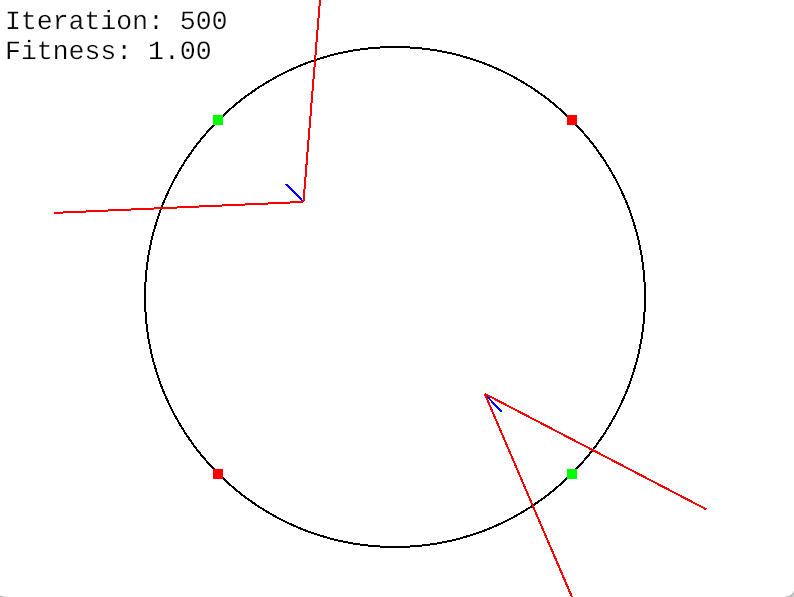
\includegraphics[width=0.4\textwidth]{Pictures/bna-xor}
       \caption{Local optima with fitness of $0.75$}
    \caption{Visualization of a solution to the \textit{XOR} problem, using the BNA algorithm with two V-neurons.}
    \label{fig:bna_xor_visual}
\end{figure}

\begin{table}
    \caption{Results of the BNA algorithm on the \textit{XOR} problem. The algorithm was tested with a maximum number of stagnant iterations of $200$.}
    \centering
    \label{tab:bna_xor}
    \begin{tabular}{ |c|c|c|c| }
        \hline
        Number of neurons & Average fitness & Average iterations & Average CPU time (s) \\
        \hline
        1 & 0.75 & 207 & 0.01 \\
        \hline
        2 & 0.79 & 174 & 0.01 \\
        \hline\hline
    \end{tabular}
\end{table}

\subsubsection{Proben1 classification problems}

The results of the BNA algorithm on the \textit{Proben1} classification problems, with different number of V-neurons and a maximum number of stagnant iterations of $200$, are presented
in \Cref{fig:bna_proben1}. Once again, the same observations as the experiment with the $(1 + 1)$ NA algorithm on the task can be made. For this configuration,
the fitness drops with the number of V-neurons, while the number of iterations and CPU time increase. The fitness on the train and test sets are very close.
Results in the case of a maximum iteration number of $10000$ are presented in \Cref{tab:bna_proben1}. This criterion allowed for higher fitness values. It was however not enough to allow
the configurations with more than three V-neurons to reach a fitness as high as the one with a single V-neuron. But the CPU time is already particularly high and would make
a further increase in the number of iterations impractical.

\begin{table}
    \caption{Results of the BNA algorithm on the \textit{Proben1 Cancer1} problem. The algorithm was tested with $10000$ iterations.}
    \centering
    \label{tab:bna_proben1}
    \begin{tabular}{ |c|c|c|c| }
        \hline
        Number of neurons & Average test fitness & Average CPU time (s) \\
        \hline
        1 & 0.96 & 199 \\
        \hline
        2 & 0.94 & 415 \\
        \hline
        3 & 0.85 & 660 \\
        \hline
        4 & 0.83 & 862 \\
        \hline\hline
    \end{tabular}
\end{table}

\begin{figure}
    \begin{center}
        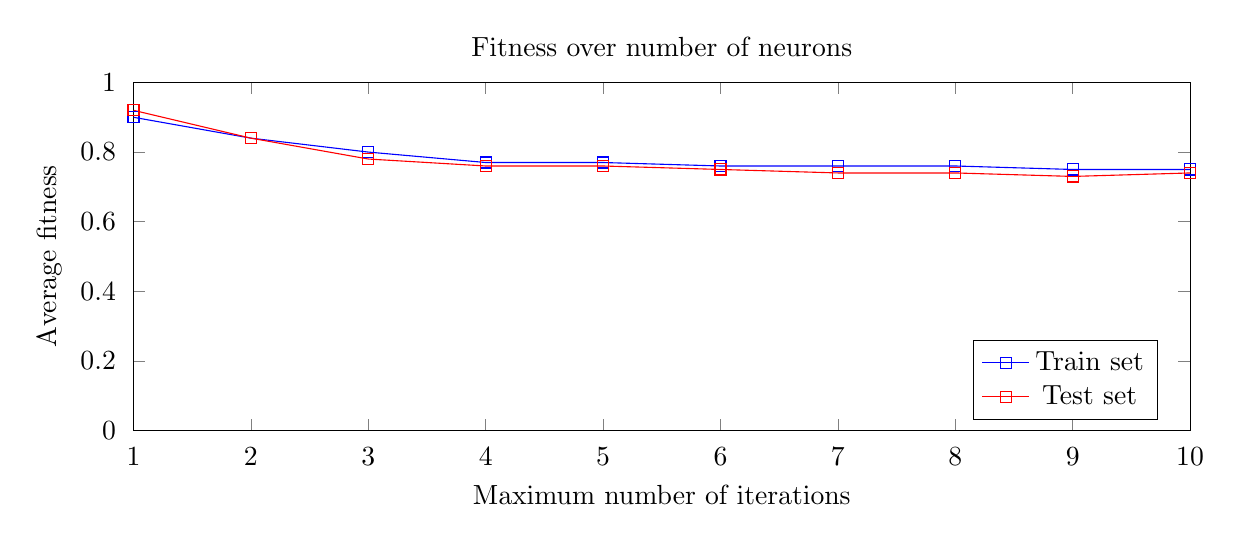
\begin{tikzpicture}
        \begin{axis}[
            width=15cm,
            height=6cm,
            title={Fitness over number of neurons},
            legend pos=south east,
            xlabel={Maximum number of iterations},
            ylabel={Average fitness},
            enlargelimits=false,
            xmin=1,
            ymin=0, ymax=1,
            ytick={0,0.2,...,1},
            xticklabel shift={.1cm},
            yticklabel shift={.1cm} ]
        ]

        \addplot[
            color=blue,
            mark=square,
            ]
            coordinates {
                (1,0.90)(2,0.84)(3,0.80)(4,0.77)(5,0.77)(6,0.76)(7,0.76)(8,0.76)(9,0.75)(10,0.75)
        };
        \addlegendentry{Train set}
        \addplot[
            color=red,
            mark=square,
            ]
            coordinates {
            (1,0.92)(2,0.84)(3,0.78)(4,0.76)(5,0.76)(6,0.75)(7,0.74)(8,0.74)(9,0.73)(10,0.74)
        };
        \addlegendentry{Test set}
        \end{axis}
        \end{tikzpicture}
        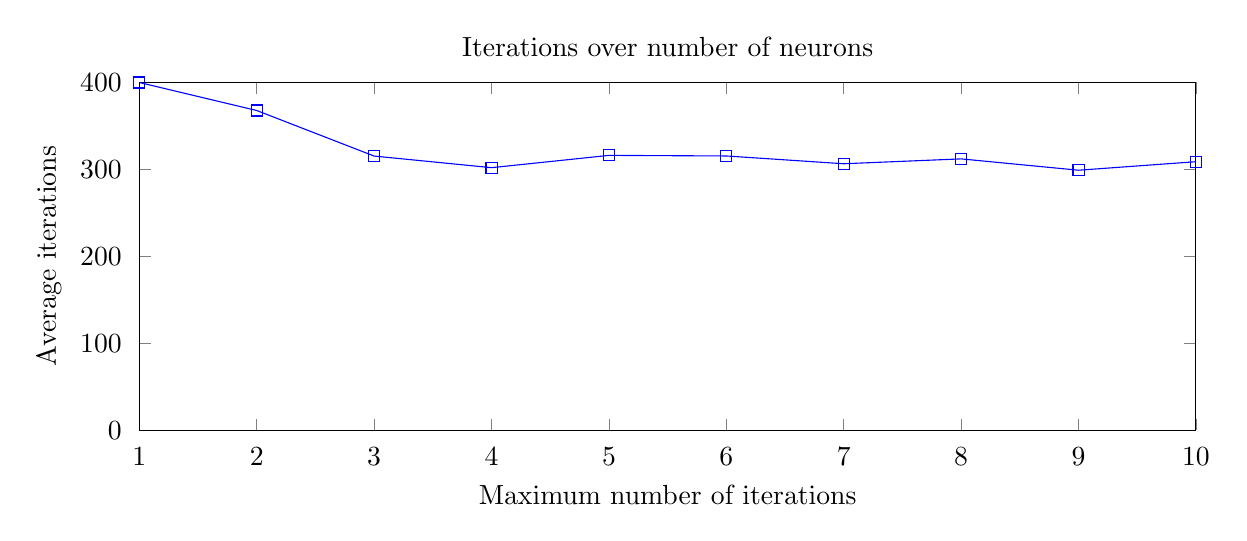
\begin{tikzpicture}
        \begin{axis}[
            width=15cm,
            height=6cm,
            legend pos=south east,
            title={Iterations over number of neurons},
            xlabel={Maximum number of iterations},
            ylabel={Average iterations},
            xmin=1,
            ymin=0,
            enlargelimits=false,
            xticklabel shift={.1cm},
            yticklabel shift={.1cm} ]
        ]

        \addplot[
            color=blue,
            mark=square,
            ]
            coordinates {
                (1,400.21)(2,367.98)(3,315.58)(4,302.22)(5,316.36)(6,315.69)(7,306.73)(8,312.33)(9,299.29)(10,309.09)
            };
        \end{axis}
        \end{tikzpicture}
        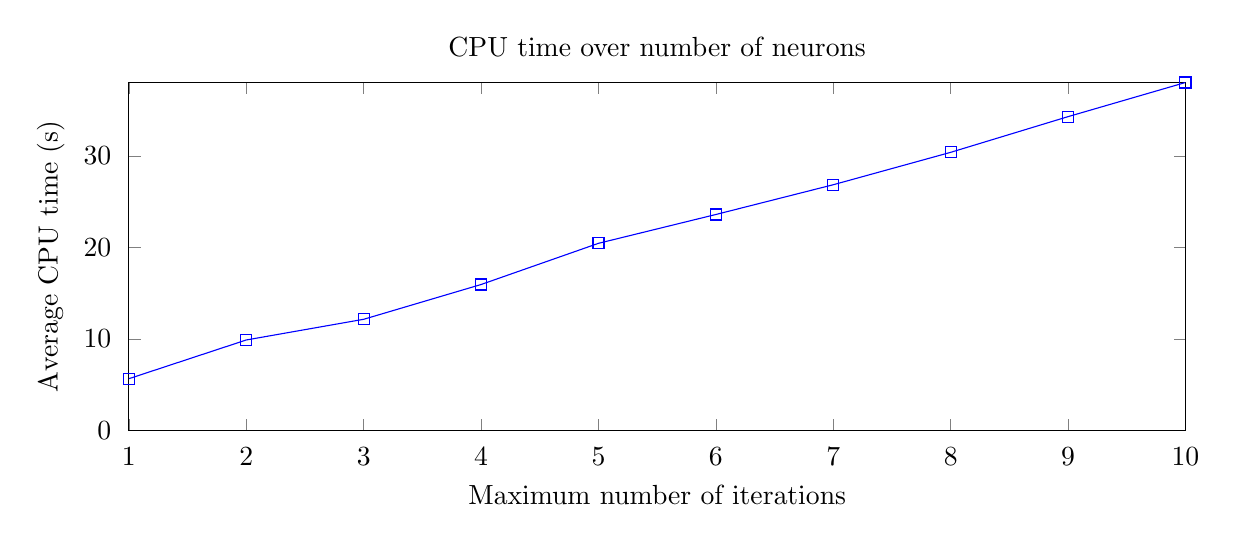
\begin{tikzpicture}
        \begin{axis}[
            width=15cm,
            height=6cm,
            legend pos=south east,
            title={CPU time over number of neurons},
            xlabel={Maximum number of iterations},
            ylabel={Average CPU time (s)},
            xmin=1,
            ymin=0,
            enlargelimits=false,
            xticklabel shift={.1cm},
            yticklabel shift={.1cm} ]
        ]

        \addplot[
            color=blue,
            mark=square,
            ]
            coordinates {
                (1,5.65)(2,9.88)(3,12.14)(4,15.94)(5,20.44)(6,23.59)(7,26.84)(8,30.38)(9,34.28)(10,38.01)
            };
        \end{axis}
        \end{tikzpicture}
    \end{center}
    \caption{Performance metrics of the BNA algorithm on the \textit{Proben1 Cancer1} benchmark, over different number of neurons.
    The evolution stopped when the fitness was $2\%$ away from the maximal fitness of $1.0$ or the maximum number of $200$ stagnant iterations was reached.}
    \label{fig:bna_proben1}
\end{figure}

\subsection{Results of the NEAT algorithm}

The NEAT algorithm can be applied to all of the selected benchmark problems. Experiments are thus conducted on the unit-sphere classification problems, the \textit{XOR}
problem, the \textit{Proben1 Cancer1} problem and the double pole balancing problem. Many parameters can be tuned for this algorithm, including:

\begin{itemize}
    \item The population size
    \item The various mutation probabilities
    \item The weights for computing the similarity between genomes
    \item The similarity threshold
    \item The parameters of the connection weights distribution
    \item The parameters of the weights perturbation distribution
    \item{The survival threshold}
\end{itemize}

\subsubsection{XOR problem}

The NEAT algorithm was first tested on the \textit{XOR} problem, as done in \cite{neat}. In addition to being used for evaluating the performance of the algorithm, different experiments aimed
at understanding the impact of some of the parameters were conducted on this benchmark. The results are presented and discussed in this section.

Compared to the $(1 + 1)$ NA and BNA algorithms discussed previously, the NEAT algorithm is population-based.
Thus, the first experiment consisted in testing different population sizes.The algorithm was evolved with a maximum number of $500$ generations. For the other parameters, the same values as in \cite{neat} were used.
The results are presented in \Cref{fig:neat_xor}. The average fitness increases with the population size, while the number of iterations decreases as a consequence because of the maximum fitness tolerance termination
criterion. However, the CPU time increases with the population size, because of the increased duration of an iteration. For example, a population of $50$ individuals resulted in a fitness of $0.82$ in $2.3$ seconds
on average, while a population of $1500$ individuals resulted in a fitness of $0.96$ in $66.6$ seconds on average.

\begin{figure}
    \begin{center}
        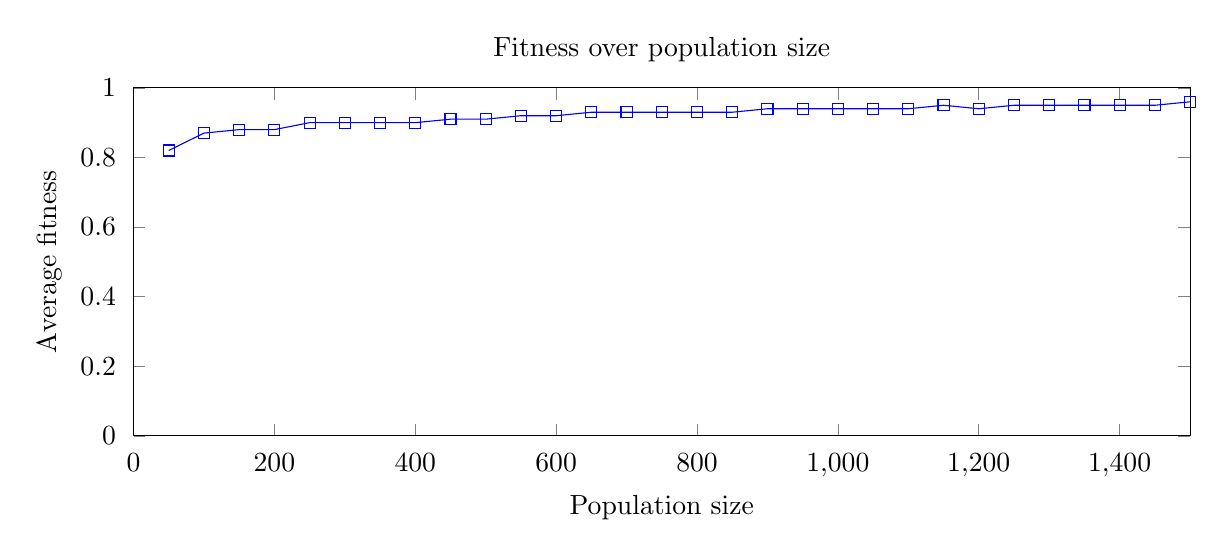
\begin{tikzpicture}
        \begin{axis}[
            width=15cm,
            height=6cm,
            title={Fitness over population size},
            legend pos=south east,
            xlabel={Population size},
            ylabel={Average fitness},
            enlargelimits=false,
            xmin=0,
            ymin=0, ymax=1,
            ytick={0,0.2,...,1},
            xticklabel shift={.1cm},
            yticklabel shift={.1cm} ]
        ]

        \addplot[
            color=blue,
            mark=square,
            ]
            coordinates {
                (50,0.82)(100,0.87)(150,0.88)(200,0.88)(250,0.90)(300,0.90)(350,0.90)(400,0.90)(450,0.91)(500,0.91)(550,0.92)(600,0.92)(650,0.93)(700,0.93)(750,0.93)(800,0.93)(850,0.93)(900,0.94)(950,0.94)(1000,0.94)(1050,0.94)(1100,0.94)(1150,0.95)(1200,0.94)(1250,0.95)(1300,0.95)(1350,0.95)(1400,0.95)(1450,0.95)(1500,0.96)
            };
        \end{axis}
        \end{tikzpicture}
        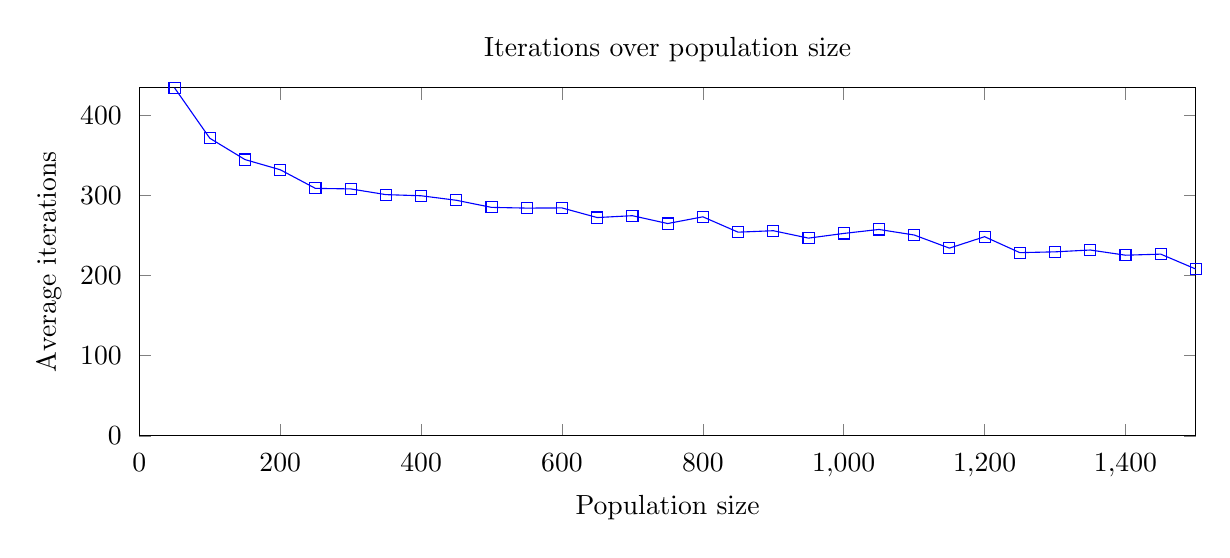
\begin{tikzpicture}
        \begin{axis}[
            width=15cm,
            height=6cm,
            legend pos=south east,
            title={Iterations over population size},
            xlabel={Population size},
            ylabel={Average iterations},
            xmin=0,
            ymin=0,
            enlargelimits=false,
            xticklabel shift={.1cm},
            yticklabel shift={.1cm} ]
        ]

        \addplot[
            color=blue,
            mark=square,
            ]
            coordinates {
                (50,434.80)(100,371.88)(150,345.18)(200,332.48)(250,309.19)(300,308.54)(350,301.39)(400,299.96)(450,294.33)(500,285.44)(550,284.55)(600,284.78)(650,272.73)(700,275.06)(750,265.25)(800,273.65)(850,254.47)(900,256.28)(950,247.01)(1000,252.89)(1050,257.86)(1100,250.93)(1150,234.51)(1200,248.80)(1250,228.87)(1300,229.88)(1350,232.16)(1400,225.69)(1450,227.02)(1500,208.31)
            };
        \end{axis}
        \end{tikzpicture}
        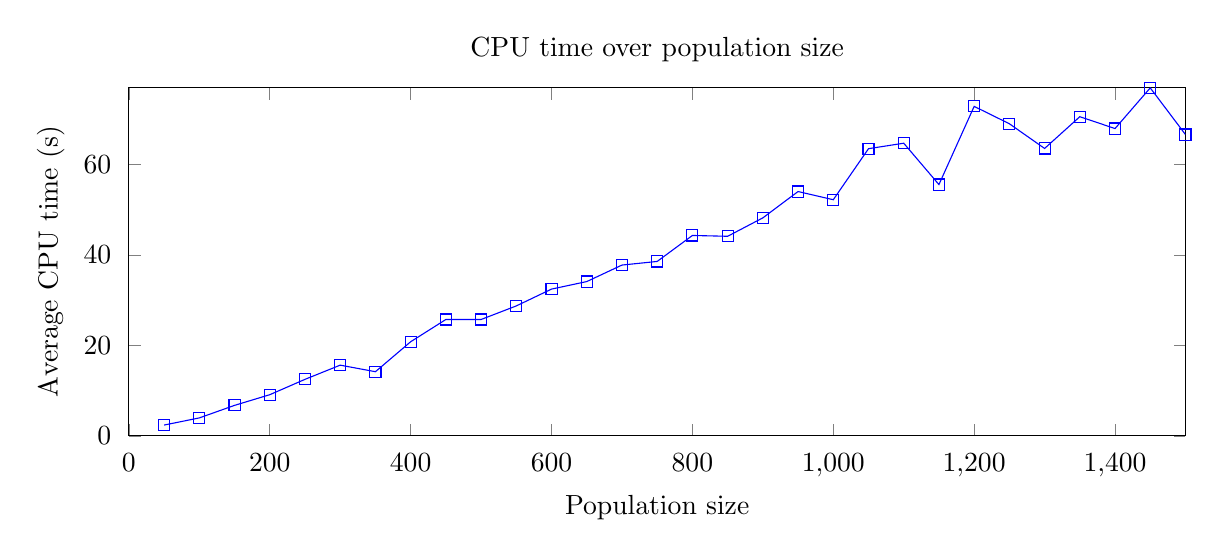
\begin{tikzpicture}
        \begin{axis}[
            width=15cm,
            height=6cm,
            legend pos=south east,
            title={CPU time over population size},
            xlabel={Population size},
            ylabel={Average CPU time (s)},
            xmin=0,
            ymin=0,
            enlargelimits=false,
            xticklabel shift={.1cm},
            yticklabel shift={.1cm} ]
        ]

        \addplot[
            color=blue,
            mark=square,
            ]
            coordinates {
                (50,2.37)(100,3.95)(150,6.72)(200,9.08)(250,12.47)(300,15.61)(350,14.16)(400,20.78)(450,25.70)(500,25.70)(550,28.70)(600,32.42)(650,34.08)(700,37.73)(750,38.53)(800,44.27)(850,44.09)(900,48.16)(950,53.98)(1000,52.17)(1050,63.45)(1100,64.66)(1150,55.52)(1200,72.80)(1250,68.96)(1300,63.50)(1350,70.52)(1400,67.90)(1450,76.89)(1500,66.57)
            };
        \end{axis}
        \end{tikzpicture}
    \end{center}
    \caption{Performance metrics of the NEAT algorithm on the \textit{XOR} benchmark, over different population sizes.
    The evolution stopped when the fitness was $2\%$ away from the maximal fitness of $1.0$ or the maximum number of $500$ generations was reached.
    The other parameters were set to the same values as in \cite{neat}.}
    \label{fig:neat_xor}
\end{figure}

One of the main characteristics of the NEAT algorithm is the speciation mechanism, where individuals are separated into species based on their similarity. The second experiment consisted in testing different
similarity thresholds, which would impact the number of species and the number of individuals in each species. Indeed, a higher similarity threshold would result in fewer species, while a lower similarity threshold
would result in more species. The results are presented in \Cref{fig:neat_xor_similarity}. The population size was set to $500$ individuals and the maximum number of generations to $500$. It can be observed that
the highest fitness values are reached in the $2.5$ to $8$ range, where the iterations and CPU time are also the lowest. The fitness was lower for the smaller similarity thresholds, where there were more
species, but with a lower number of individuals in each species. Starting from thresholds greater than $8$, the performances remain stable, which is because of these values resulting in a single species.

\begin{figure}
    \begin{center}
        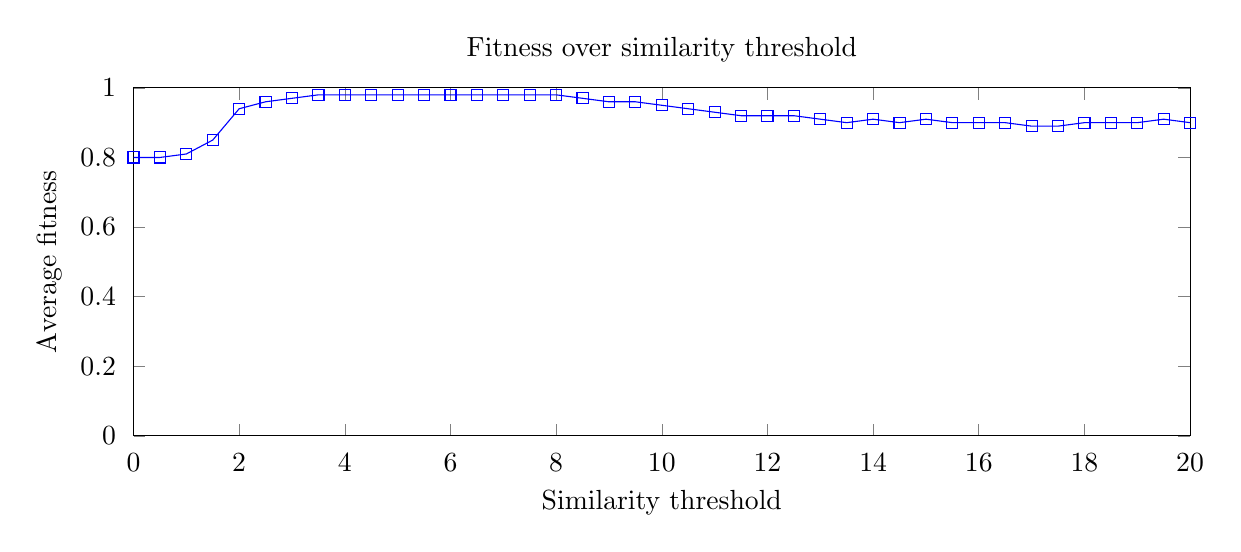
\begin{tikzpicture}
        \begin{axis}[
            width=15cm,
            height=6cm,
            title={Fitness over similarity threshold},
            legend pos=south east,
            xlabel={Similarity threshold},
            ylabel={Average fitness},
            enlargelimits=false,
            xmin=0,
            ymin=0, ymax=1,
            ytick={0,0.2,...,1},
            xticklabel shift={.1cm},
            yticklabel shift={.1cm} ]
        ]

        \addplot[
            color=blue,
            mark=square,
            ]
            coordinates {
                (0.0,0.80)(0.5,0.80)(1.0,0.81)(1.5,0.85)(2.0,0.94)(2.5,0.96)(3.0,0.97)(3.5,0.98)(4.0,0.98)(4.5,0.98)(5.0,0.98)(5.5,0.98)(6.0,0.98)(6.5,0.98)(7.0,0.98)(7.5,0.98)(8.0,0.98)(8.5,0.97)(9.0,0.96)(9.5,0.96)(10.0,0.95)(10.5,0.94)(11.0,0.93)(11.5,0.92)(12.0,0.92)(12.5,0.92)(13.0,0.91)(13.5,0.90)(14.0,0.91)(14.5,0.90)(15.0,0.91)(15.5,0.90)(16.0,0.90)(16.5,0.90)(17.0,0.89)(17.5,0.89)(18.0,0.90)(18.5,0.90)(19.0,0.90)(19.5,0.91)(20.0,0.90)
            };
        \end{axis}
        \end{tikzpicture}
        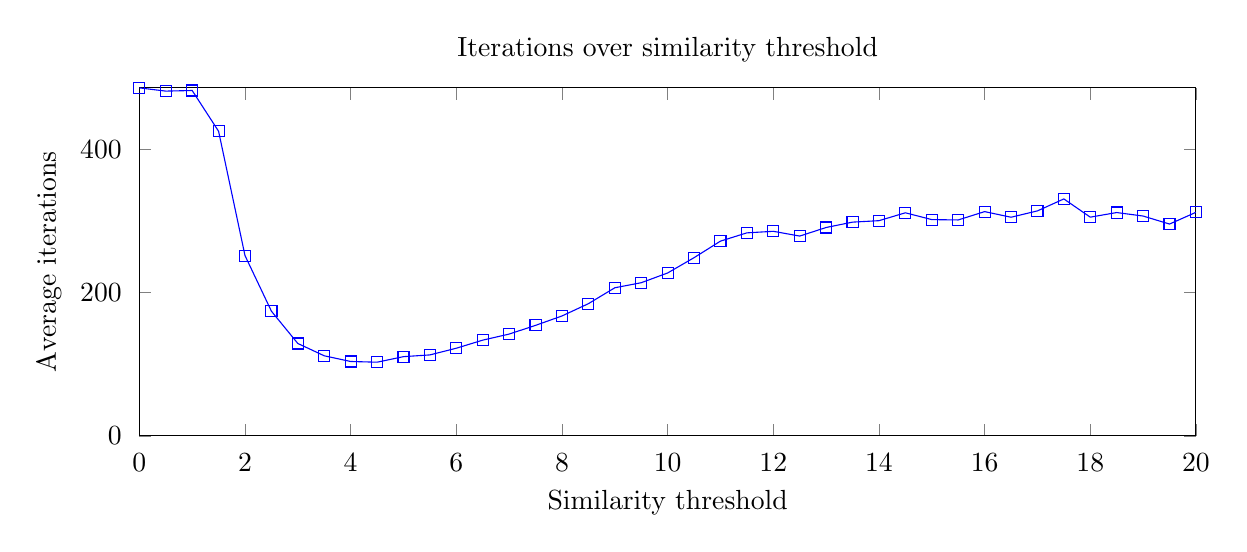
\begin{tikzpicture}
        \begin{axis}[
            width=15cm,
            height=6cm,
            legend pos=south east,
            title={Iterations over similarity threshold},
            xlabel={Similarity threshold},
            ylabel={Average iterations},
            xmin=0,
            ymin=0,
            enlargelimits=false,
            xticklabel shift={.1cm},
            yticklabel shift={.1cm} ]
        ]

        \addplot[
            color=blue,
            mark=square,
            ]
            coordinates {
                (0.0,486.12)(0.5,481.60)(1.0,482.44)(1.5,425.45)(2.0,251.76)(2.5,174.06)(3.0,128.96)(3.5,111.75)(4.0,103.80)(4.5,102.82)(5.0,110.56)(5.5,113.00)(6.0,122.35)(6.5,133.64)(7.0,142.11)(7.5,154.28)(8.0,167.42)(8.5,184.58)(9.0,206.81)(9.5,213.87)(10.0,227.49)(10.5,248.85)(11.0,271.99)(11.5,283.54)(12.0,285.71)(12.5,279.04)(13.0,291.03)(13.5,298.53)(14.0,300.55)(14.5,311.57)(15.0,302.06)(15.5,301.56)(16.0,313.23)(16.5,305.37)(17.0,314.23)(17.5,330.94)(18.0,305.47)(18.5,311.92)(19.0,307.03)(19.5,295.83)(20.0,312.24)
            };
        \end{axis}
        \end{tikzpicture}
        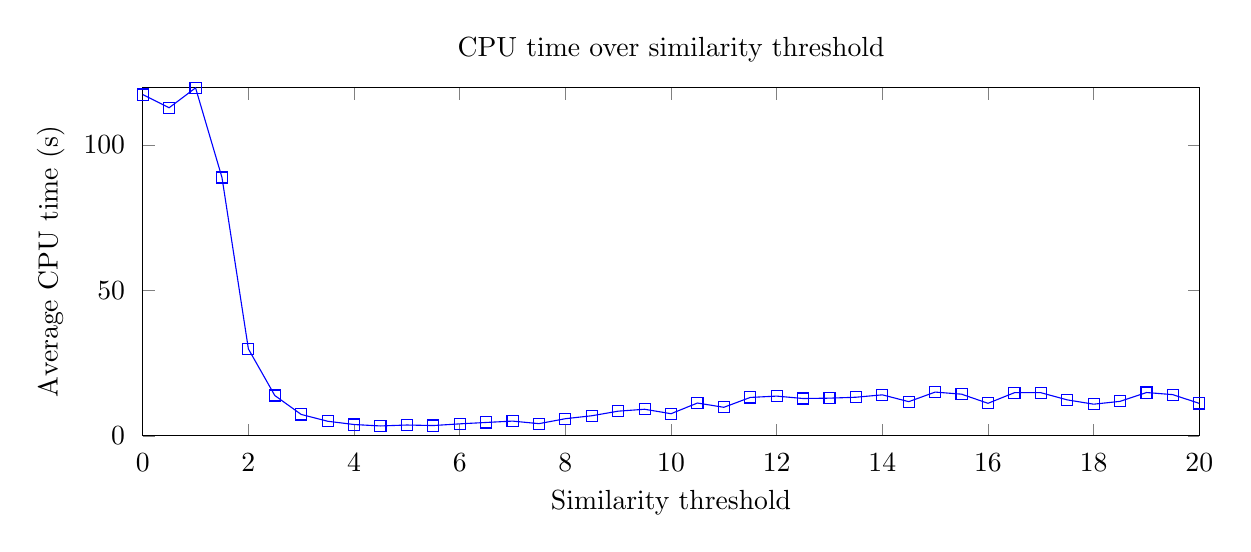
\begin{tikzpicture}
        \begin{axis}[
            width=15cm,
            height=6cm,
            legend pos=south east,
            title={CPU time over similarity threshold},
            xlabel={Similarity threshold},
            ylabel={Average CPU time (s)},
            xmin=0,
            ymin=0,
            enlargelimits=false,
            xticklabel shift={.1cm},
            yticklabel shift={.1cm} ]
        ]

        \addplot[
            color=blue,
            mark=square,
            ]
            coordinates {
                (0.0,117.27)(0.5,112.74)(1.0,119.57)(1.5,88.77)(2.0,29.85)(2.5,13.84)(3.0,7.33)(3.5,5.00)(4.0,3.87)(4.5,3.38)(5.0,3.70)(5.5,3.52)(6.0,4.10)(6.5,4.58)(7.0,5.05)(7.5,4.17)(8.0,5.87)(8.5,6.88)(9.0,8.46)(9.5,9.12)(10.0,7.59)(10.5,11.26)(11.0,9.79)(11.5,13.18)(12.0,13.64)(12.5,12.81)(13.0,12.93)(13.5,13.25)(14.0,14.07)(14.5,11.73)(15.0,15.02)(15.5,14.30)(16.0,11.16)(16.5,14.81)(17.0,14.81)(17.5,12.34)(18.0,10.86)(18.5,11.83)(19.0,14.87)(19.5,14.14)(20.0,11.12)
            };
        \end{axis}
        \end{tikzpicture}
    \end{center}
    \caption{Performance metrics of the NEAT algorithm on the \textit{XOR} benchmark, over different similarity thresholds.
    The evolution stopped when the fitness was $2\%$ away from the maximal fitness of $1.0$ or the maximum number of $500$ generations was reached.
    The other parameters were set to the same values as in \cite{neat}.}
    \label{fig:neat_xor_similarity}
\end{figure}

Another parameter is the maximum number of generations (or iterations).\Cref{fig:neat_xor_generations} presents the results of the algorithm on the problem, with different maximum numbers of generations,
a population size of $300$ and a similarity threshold of $8.0$. As expected, all three metrics increase with the number of generations, particularly in the $50$ to $200$ range, before stabilizing.
The algorithm was able to solve the problem in less than $150$ generations on average.

\begin{figure}
    \begin{center}
        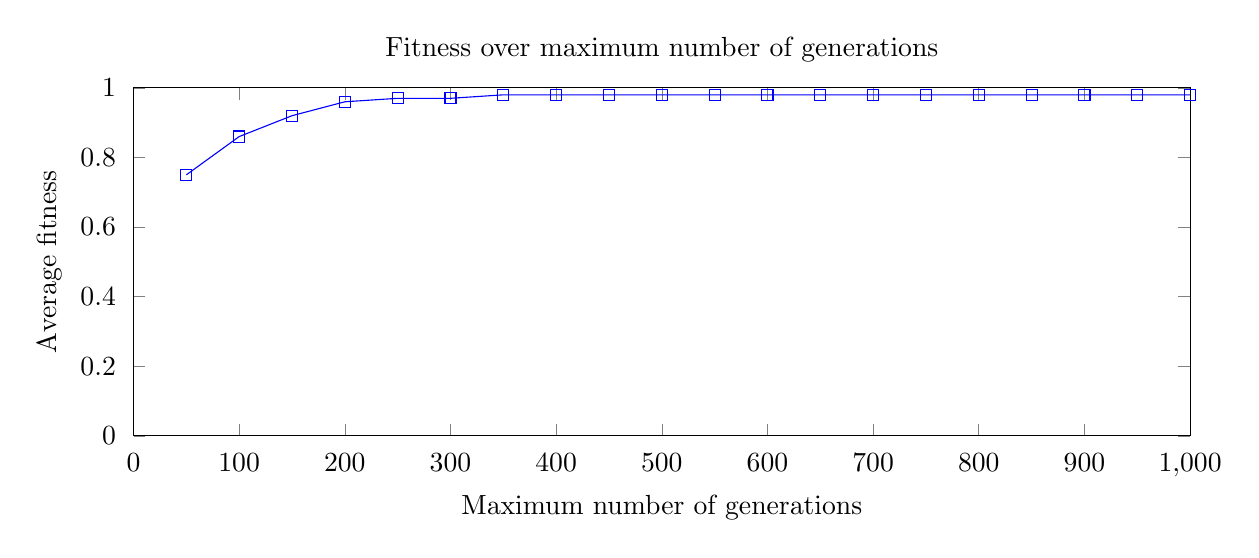
\begin{tikzpicture}
        \begin{axis}[
            width=15cm,
            height=6cm,
            title={Fitness over maximum number of generations},
            xlabel={Maximum number of generations},
            ylabel={Average fitness},
            enlargelimits=false,
            xmin=0,
            ymin=0, ymax=1,
            ytick={0,0.2,...,1},
            xticklabel shift={.1cm},
            yticklabel shift={.1cm} ]
        ]

        \addplot[
            color=blue,
            mark=square,
            ]
            coordinates {
                (50,0.75)(100,0.86)(150,0.92)(200,0.96)(250,0.97)(300,0.97)(350,0.98)(400,0.98)(450,0.98)(500,0.98)(550,0.98)(600,0.98)(650,0.98)(700,0.98)(750,0.98)(800,0.98)(850,0.98)(900,0.98)(950,0.98)(1000,0.98)
            };
        \end{axis}
        \end{tikzpicture}
        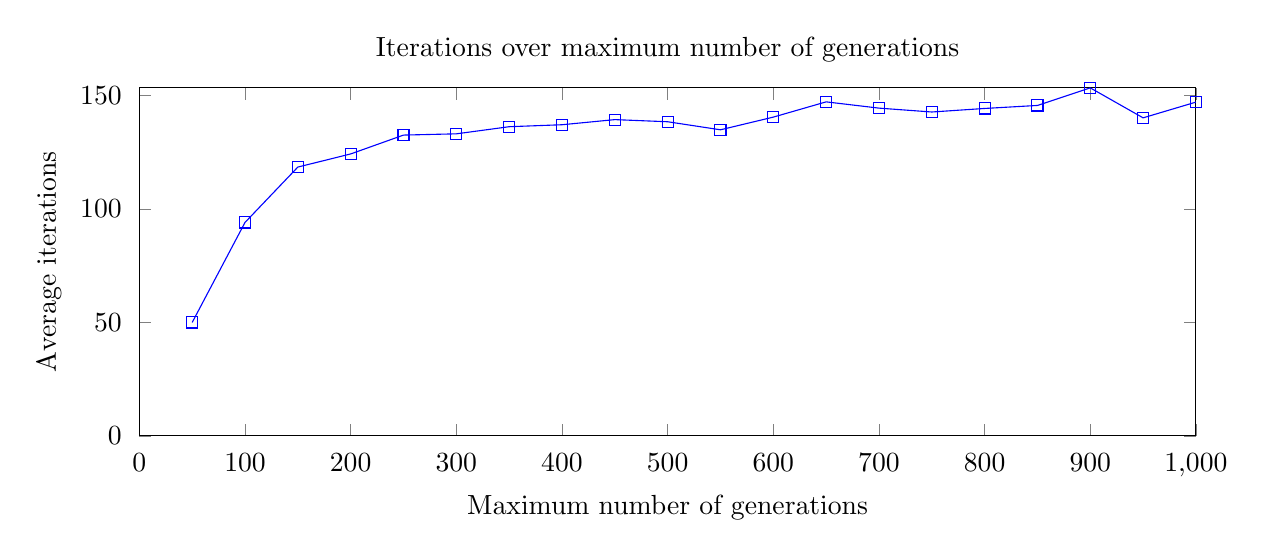
\begin{tikzpicture}
        \begin{axis}[
            width=15cm,
            height=6cm,
            legend pos=south east,
            title={Iterations over maximum number of generations},
            xlabel={Maximum number of generations},
            ylabel={Average iterations},
            xmin=0,
            ymin=0,
            enlargelimits=false,
            xticklabel shift={.1cm},
            yticklabel shift={.1cm} ]
        ]

        \addplot[
            color=blue,
            mark=square,
            ]
            coordinates {
                (50,49.98)(100,94.09)(150,118.51)(200,124.30)(250,132.62)(300,133.17)(350,136.31)(400,137.18)(450,139.44)(500,138.50)(550,134.95)(600,140.54)(650,147.27)(700,144.51)(750,142.80)(800,144.36)(850,145.69)(900,153.44)(950,140.22)(1000,147.16)
            };
        \end{axis}
        \end{tikzpicture}
        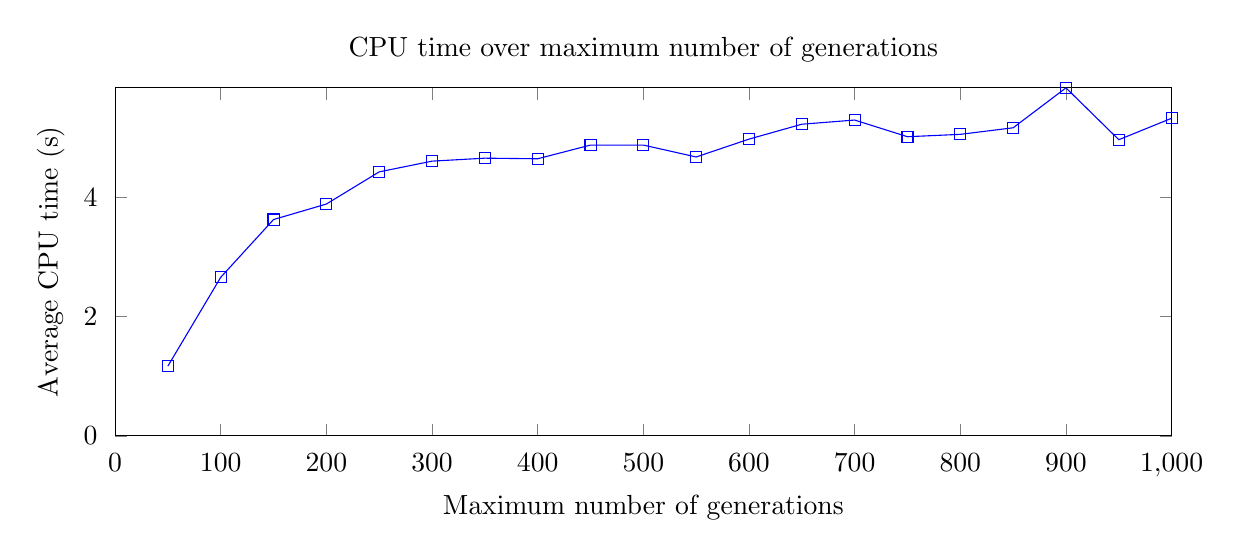
\begin{tikzpicture}
        \begin{axis}[
            width=15cm,
            height=6cm,
            legend pos=south east,
            title={CPU time over maximum number of generations},
            xlabel={Maximum number of generations},
            ylabel={Average CPU time (s)},
            xmin=0,
            ymin=0,
            enlargelimits=false,
            xticklabel shift={.1cm},
            yticklabel shift={.1cm} ]
        ]

        \addplot[
            color=blue,
            mark=square,
            ]
            coordinates {
                (50,1.17)(100,2.66)(150,3.63)(200,3.89)(250,4.43)(300,4.61)(350,4.66)(400,4.65)(450,4.88)(500,4.88)(550,4.68)(600,4.98)(650,5.23)(700,5.30)(750,5.02)(800,5.06)(850,5.17)(900,5.84)(950,4.97)(1000,5.33)
            };
        \end{axis}
        \end{tikzpicture}
    \end{center}
    \caption{Performance metrics of the NEAT algorithm on the \textit{XOR} benchmark, over different maximum generations.
    The evolution stopped when the fitness was $2\%$ away from the maximal fitness of $1.0$ or the maximum number of generations was reached.
    The other parameters were set to the same values as in \cite{neat}.}
    \label{fig:neat_xor_generations}
\end{figure}

Finally, the most important characteristic of the algorithm is its ability to evolve topologies, by adding connections or nodes through mutations. This final experiment consisted in testing different
values for the probability of adding a new node (and its connections) to the genome. The results are presented in \Cref{fig:neat_xor_probabilities}. The population size was set to $300$ individuals,
the similarity threshold to $8.0$ and the maximum number of generations to $300$. As it was the case for the other parameters, there is a range of values for the new node mutation probability that
result in the best performance, in this case around the value of $0.05$, which is consistent with the choice made in \cite{neat} of $0.03$. Furthermore, for a value of $0.0$, no hidden nodes are added
to the network, and because of the starting topology only consists in a input and output layer, the algorithm cannot solve the problem, which requires hidden neurons. For higher values,
too many nodes are added, which results in an increase in the CPU time, and a decrease in the fitness, because of the increased complexity of the networks.

% TODO minimal network figure

\begin{figure}
    \begin{center}
        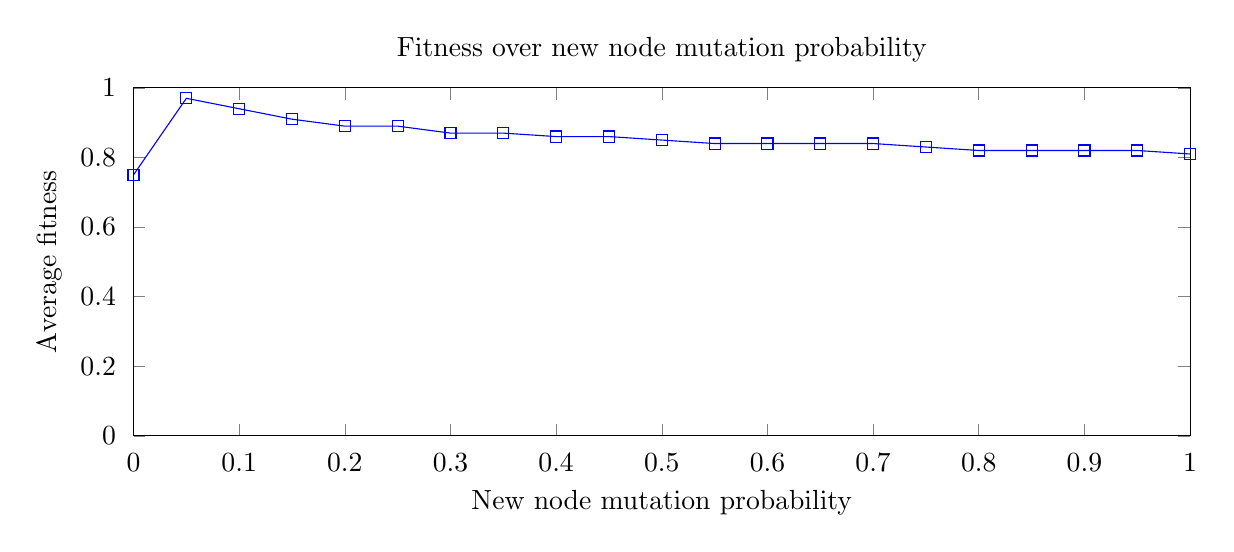
\begin{tikzpicture}
        \begin{axis}[
            width=15cm,
            height=6cm,
            title={Fitness over new node mutation probability},
            xlabel={New node mutation probability},
            ylabel={Average fitness},
            enlargelimits=false,
            xmin=0,
            ymin=0, ymax=1,
            ytick={0,0.2,...,1},
            xticklabel shift={.1cm},
            yticklabel shift={.1cm} ]
        ]

        \addplot[
            color=blue,
            mark=square,
            ]
            coordinates {
                (0.00,0.75)(0.05,0.97)(0.10,0.94)(0.15,0.91)(0.20,0.89)(0.25,0.89)(0.30,0.87)(0.35,0.87)(0.40,0.86)(0.45,0.86)(0.50,0.85)(0.55,0.84)(0.60,0.84)(0.65,0.84)(0.70,0.84)(0.75,0.83)(0.80,0.82)(0.85,0.82)(0.90,0.82)(0.95,0.82)(1.00,0.81)
            };
        \end{axis}
        \end{tikzpicture}
        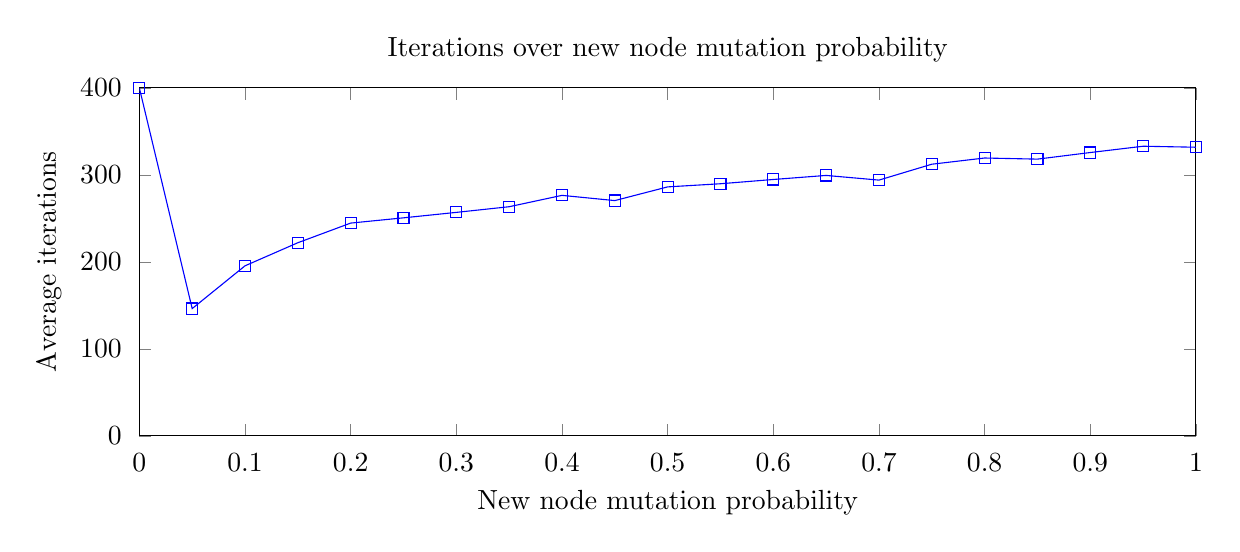
\begin{tikzpicture}
        \begin{axis}[
            width=15cm,
            height=6cm,
            legend pos=south east,
            title={Iterations over new node mutation probability},
            xlabel={New node mutation probability},
            ylabel={Average iterations},
            xmin=0,
            ymin=0,
            enlargelimits=false,
            xticklabel shift={.1cm},
            yticklabel shift={.1cm} ]
        ]

        \addplot[
            color=blue,
            mark=square,
            ]
            coordinates {
                (0.00,400.00)(0.05,146.24)(0.10,195.41)(0.15,221.95)(0.20,244.54)(0.25,250.58)(0.30,256.85)(0.35,263.36)(0.40,276.41)(0.45,270.41)(0.50,286.16)(0.55,289.77)(0.60,294.68)(0.65,299.33)(0.70,293.96)(0.75,312.23)(0.80,319.36)(0.85,318.08)(0.90,325.66)(0.95,332.90)(1.00,331.76)
            };
        \end{axis}
        \end{tikzpicture}
        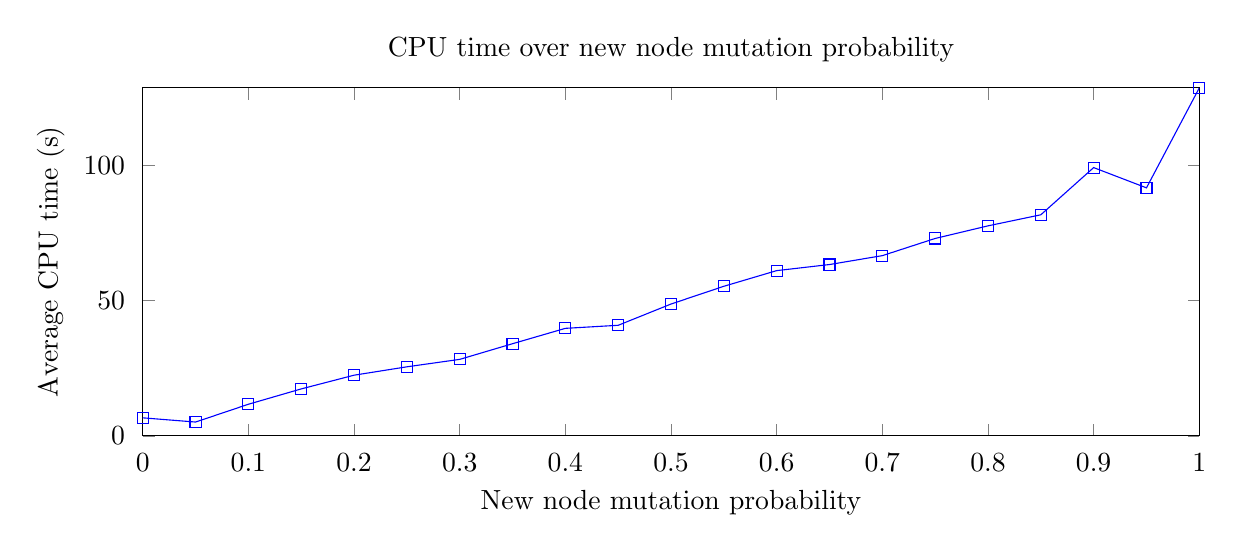
\begin{tikzpicture}
        \begin{axis}[
            width=15cm,
            height=6cm,
            legend pos=south east,
            title={CPU time over new node mutation probability},
            xlabel={New node mutation probability},
            ylabel={Average CPU time (s)},
            xmin=0,
            ymin=0,
            enlargelimits=false,
            xticklabel shift={.1cm},
            yticklabel shift={.1cm} ]
        ]

        \addplot[
            color=blue,
            mark=square,
            ]
            coordinates {
                (0.00,6.64)(0.05,5.08)(0.10,11.66)(0.15,17.33)(0.20,22.40)(0.25,25.50)(0.30,28.25)(0.35,34.04)(0.40,39.72)(0.45,40.85)(0.50,48.71)(0.55,55.27)(0.60,61.06)(0.65,63.31)(0.70,66.60)(0.75,72.95)(0.80,77.61)(0.85,81.70)(0.90,99.15)(0.95,91.66)(1.00,128.62)
            };
        \end{axis}
        \end{tikzpicture}
    \end{center}
    \caption{Performance metrics of the NEAT algorithm on the \textit{XOR} benchmark, over different new node mutation probabilities.
    The evolution stopped when the fitness was $2\%$ away from the maximal fitness of $1.0$ or the maximum number of generations was reached.
    The other parameters were set to the same values as in \cite{neat}.}
    \label{fig:neat_xor_probabilities}
\end{figure}

\subsubsection{Double pole balancing problem}

The NEAT algorithm was also tested on the double pole balancing control problem.
The configuration described in \cite{neat} was found to be particularly efficient on this task, the results using it are presented in \Cref{tab:nneat_pole}.
The algorithm was always able to solve the problem, and in $11$ iterations on average. The CPU time was $6.19$ seconds on average, which is high when compared to the previous benchmarks,
when considering the same number of iterations. This is because of the fitness evaluation being more computationally expensive for this problem, as it requires simulating the pole balancing
system.

\begin{table}
    \caption{Results of the NEAT algorithm on the \textit{Pole balancing} problem. The algorithm was tested with the same configuration as in \cite{neat}, with a maximum of $100$ generations.}
    \centering
    \label{tab:nneat_pole}
    \begin{tabular}{ |c|c|c| }
        \hline
        Average fitness & Average iterations & Average CPU time (s) \\
        \hline
        1.00 & 11 & 6.19 \\
        \hline\hline
    \end{tabular}
\end{table}

\subsubsection{Unit sphere classification problems}

The algorithm was tested on the \textit{Half}, \textit{Quarter} and \textit{TwoQuarters} and \textit{LocalOpt} unit sphere classification problems. The performance metrics are presented in \Cref{tab:nneat_sphere}.

% TODO Config in Appendix

\begin{table}
    \caption{Results of the NEAT algorithm on the unit-sphere classification problems.}
    \centering
    \label{tab:nneat_sphere}
    \begin{tabular}{ |c|c|c|c| }
        \hline
        Problem & Average fitness & Average iterations & Average CPU time (s) \\
        \hline
        Half & 0.98 & 24 & 127 \\
        \hline
        Quarter & 0.98 & 9 & 39 \\
        \hline
        TwoQuarters & 0.74 & 100 & 935 \\
        \hline
        LocalOpt & 0.65 & 100 & 1134 \\
        \hline\hline
    \end{tabular}
\end{table}

\subsubsection{Proben1 classification problems}

Finally, the NEAT algorithm was tested on the \textit{Proben1 Cancer1} problem. The results are presented in \Cref{tab:neat_proben1}.
The algorithm was able to solve the problem in all of the runs, in the particularly low number of 7 Iterations on average. However, the CPU time was high. As a matter of fact, it was
higher than for the pole balancing problem, with an average of $35.8$ seconds, despite the lower number of iterations.

% TODO Config in Appendix

\begin{table}
    \caption{Results of the NEAT algorithm on the \textit{Proben1 Cancer1} problem.}
    \centering
    \label{tab:neat_proben1}
    \begin{tabular}{ |c|c|c| }
        \hline
        Average test set fitness & Average iterations & Average CPU time (s) \\
        \hline
        0.98 & 7 & 35.8 \\
        \hline\hline
    \end{tabular}
\end{table}

\subsection{Results of the CMA-ES algorithm}

The CMA-ES algorithm can be used to evolve the connection weights of networks, which can be used to solve all the selected benchmark problems. Experiments are thus conducted on the unit-sphere
classification problems, the \textit{XOR} problem, the \textit{Proben1 Cancer1} problem and the double pole balancing problem. Many parameters can be tuned for this algorithm.
However, the focus was put on the fixed network topologies, while using the default parameters for the algorithm provided by the \texttt{cmaes}
crate \footnote{\url{https://docs.rs/cmaes/latest/cmaes/options/struct.CMAESOptions.html}}. For all of the following experiments, the sigmoid activation function was used for hidden
and output neurons.

\subsubsection{XOR problem}

The CMA-ES algorithm was first tested on the evolution of connection weights for the \textit{XOR} problem.
Fully connected networks with $0$ to $5$ hidden neurons were tested. The results are presented in \Cref{fig:cmaes_xor}.
For $0$ to $2$ hidden neurons, the algorithm was only able to find the $0.75$ fitness local optima. The number of iterations and the CPU time increased with the number of hidden neurons,
but both remained particularly low. For the $4$ and $5$ hidden neurons case, the algorithm was able to find an optimal solution in the majority of the runs.

\begin{figure}
    \begin{center}
        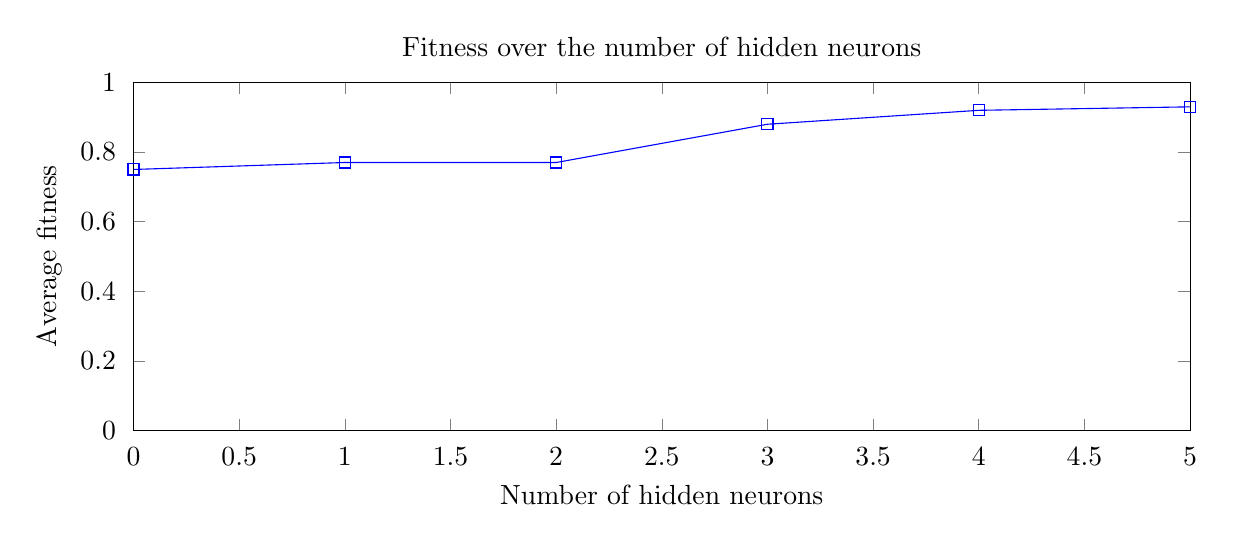
\begin{tikzpicture}
        \begin{axis}[
            width=15cm,
            height=6cm,
            title={Fitness over the number of hidden neurons},
            xlabel={Number of hidden neurons},
            ylabel={Average fitness},
            enlargelimits=false,
            xmin=0,
            ymin=0, ymax=1,
            ytick={0,0.2,...,1},
            xticklabel shift={.1cm},
            yticklabel shift={.1cm} ]
        ]

        \addplot[
            color=blue,
            mark=square,
            ]
            coordinates {
                (0,0.75)(1,0.77)(2,0.77)(3,0.88)(4,0.92)(5,0.93)
            };
        \end{axis}
        \end{tikzpicture}
        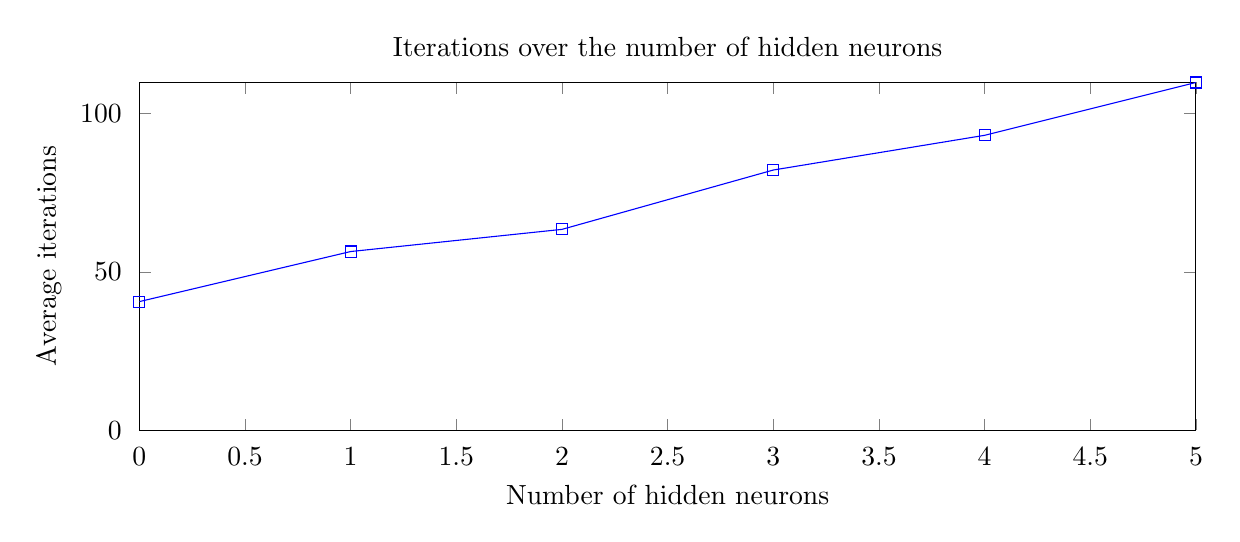
\begin{tikzpicture}
        \begin{axis}[
            width=15cm,
            height=6cm,
            legend pos=south east,
            title={Iterations over the number of hidden neurons},
            xlabel={Number of hidden neurons},
            ylabel={Average iterations},
            xmin=0,
            ymin=0,
            enlargelimits=false,
            xticklabel shift={.1cm},
            yticklabel shift={.1cm} ]
        ]

        \addplot[
            color=blue,
            mark=square,
            ]
            coordinates {
                (0,40.67)(1,56.48)(2,63.48)(3,82.22)(4,93.18)(5,109.86)
            };
        \end{axis}
        \end{tikzpicture}
        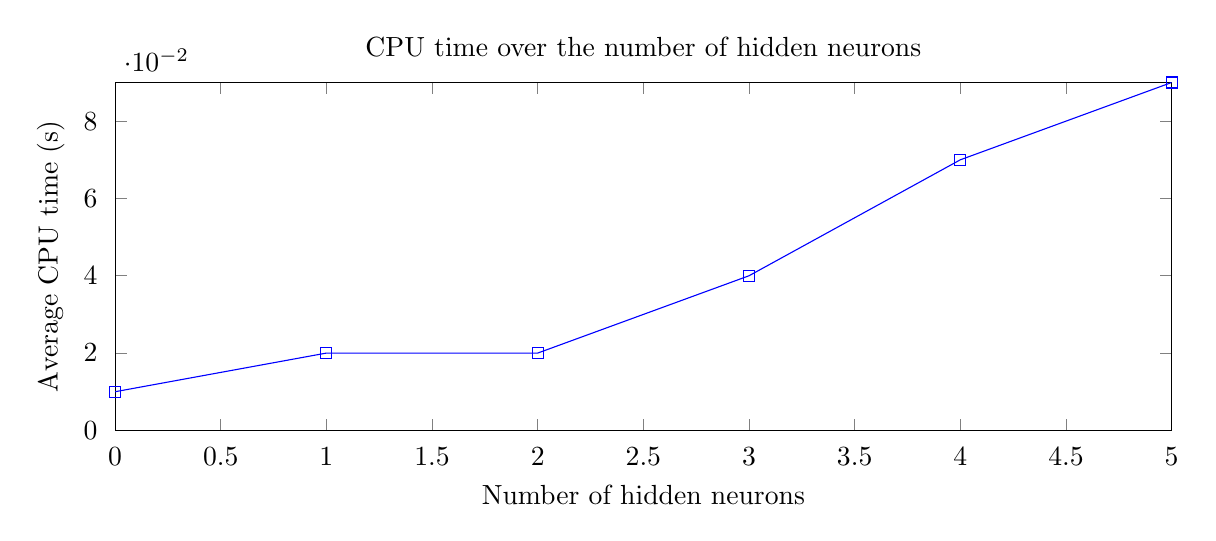
\begin{tikzpicture}
        \begin{axis}[
            width=15cm,
            height=6cm,
            legend pos=south east,
            title={CPU time over the number of hidden neurons},
            xlabel={Number of hidden neurons},
            ylabel={Average CPU time (s)},
            xmin=0,
            ymin=0,
            enlargelimits=false,
            xticklabel shift={.1cm},
            yticklabel shift={.1cm} ]
        ]

        \addplot[
            color=blue,
            mark=square,
            ]
            coordinates {
                (0,0.01)(1,0.02)(2,0.02)(3,0.04)(4,0.07)(5,0.09)
            };
        \end{axis}
        \end{tikzpicture}
    \end{center}
    \caption{Performance metrics of the CMA-ES algorithm on the \textit{XOR} benchmark, over different number of hidden neurons.}
    \label{fig:cmaes_xor}
\end{figure}

\subsubsection{Double pole balancing problem}

Fully connected networks with $0$ to $6$ hidden neurons were considered for the double pole balancing problem. The results are presented in \Cref{fig:cmaes_pole}.
The main observation which can be made is that when initially switching from a two-layers to a three-layers network, the fitness drops significantly from $0.67$ to $0.1$ but
increases as more hidden neurons are added and eventually reaches $0.89$ for $6$ hidden neurons. Furthermore, in addition to the lower fitness values compared to the simpler \textit{XOR} problem,
the number of iterations and CPU time were significantly higher, with the CPU time reaching $300$ seconds for $6$ hidden neurons.

\begin{figure}
    \begin{center}
        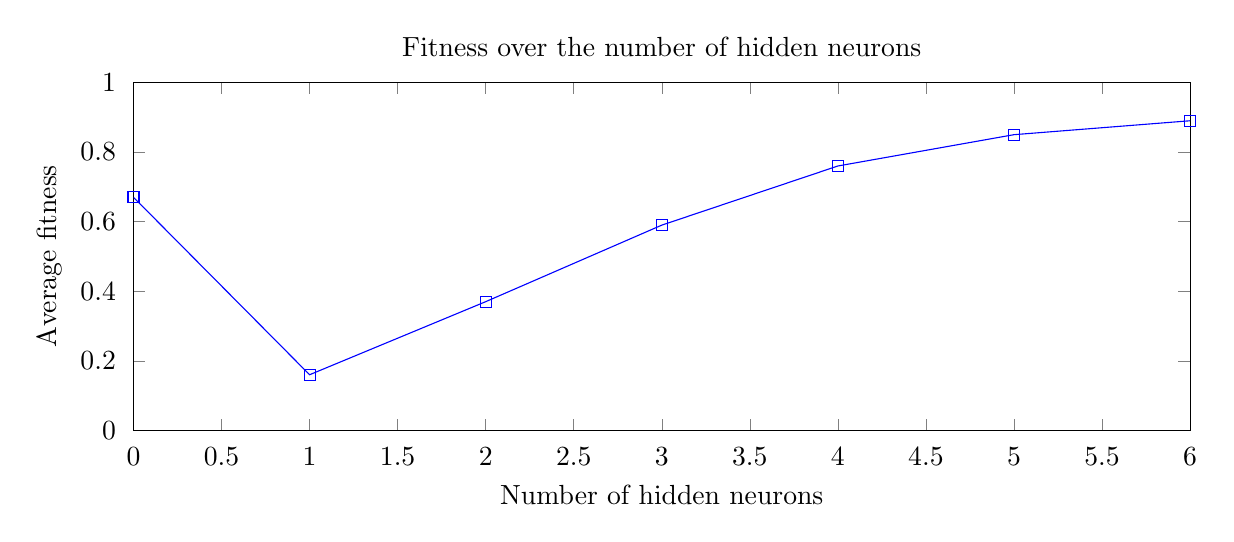
\begin{tikzpicture}
        \begin{axis}[
            width=15cm,
            height=6cm,
            title={Fitness over the number of hidden neurons},
            xlabel={Number of hidden neurons},
            ylabel={Average fitness},
            enlargelimits=false,
            xmin=0,
            ymin=0, ymax=1,
            ytick={0,0.2,...,1},
            xticklabel shift={.1cm},
            yticklabel shift={.1cm} ]
        ]

        \addplot[
            color=blue,
            mark=square,
            ]
            coordinates {
                (0,0.67)(1,0.16)(2,0.37)(3,0.59)(4,0.76)(5,0.85)(6,0.89)
            };
        \end{axis}
        \end{tikzpicture}
        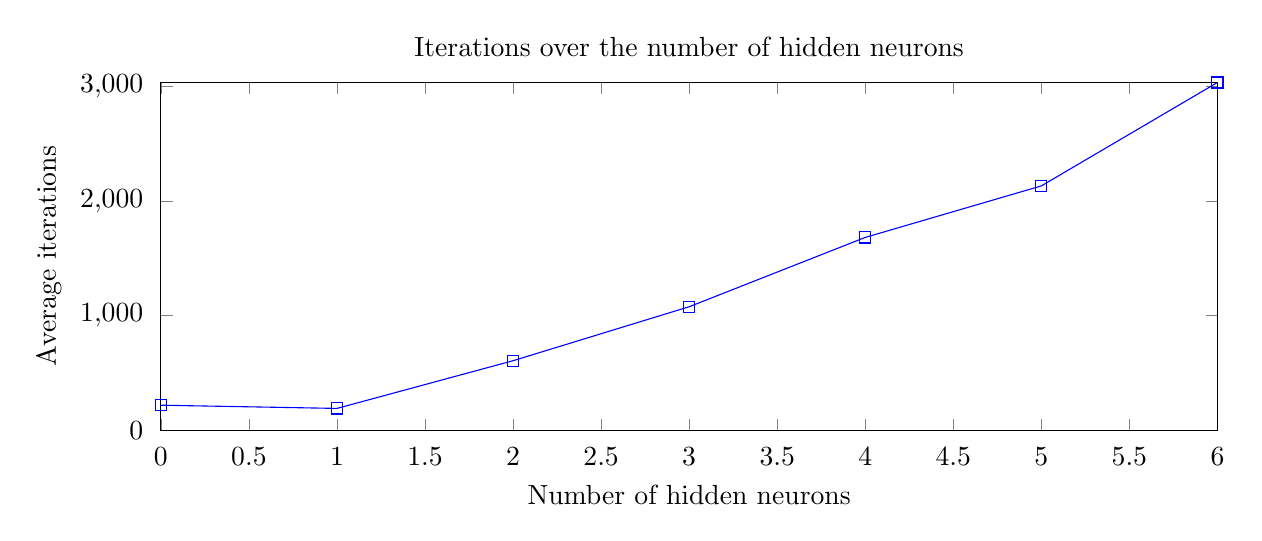
\begin{tikzpicture}
        \begin{axis}[
            width=15cm,
            height=6cm,
            legend pos=south east,
            title={Iterations over the number of hidden neurons},
            xlabel={Number of hidden neurons},
            ylabel={Average iterations},
            xmin=0,
            ymin=0,
            enlargelimits=false,
            xticklabel shift={.1cm},
            yticklabel shift={.1cm} ]
        ]

        \addplot[
            color=blue,
            mark=square,
            ]
            coordinates {
                (0,219.50)(1,191.51)(2,607.18)(3,1077.43)(4,1681.43)(5,2130.26)(6,3031.31)
            };
        \end{axis}
        \end{tikzpicture}
        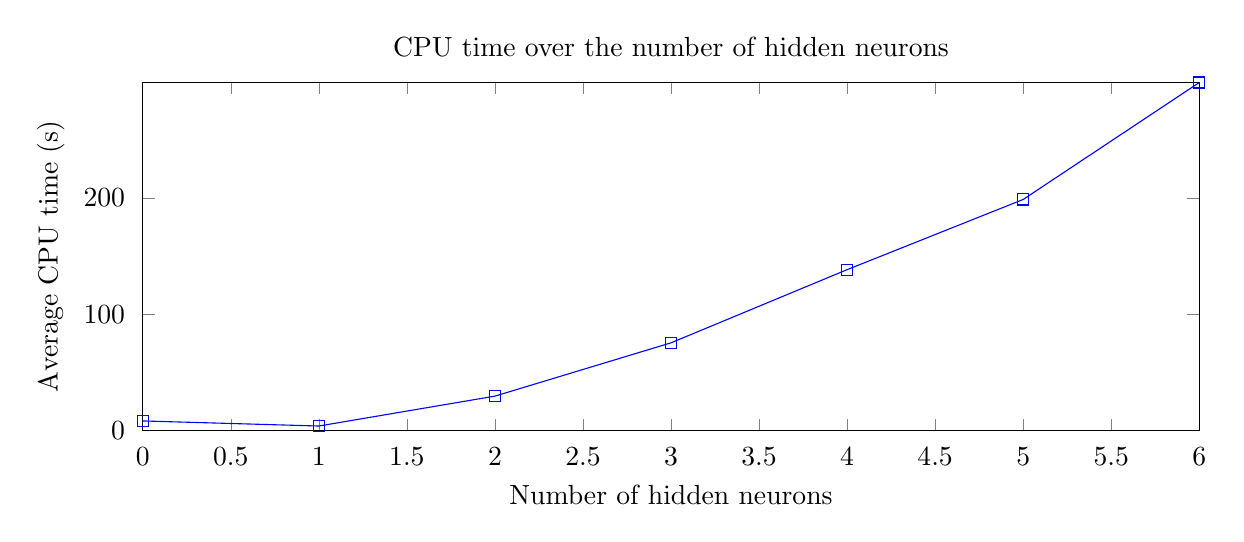
\begin{tikzpicture}
        \begin{axis}[
            width=15cm,
            height=6cm,
            legend pos=south east,
            title={CPU time over the number of hidden neurons},
            xlabel={Number of hidden neurons},
            ylabel={Average CPU time (s)},
            xmin=0,
            ymin=0,
            enlargelimits=false,
            xticklabel shift={.1cm},
            yticklabel shift={.1cm} ]
        ]

        \addplot[
            color=blue,
            mark=square,
            ]
            coordinates {
                (0,8.15)(1,3.77)(2,29.49)(3,75.35)(4,138.29)(5,198.70)(6,299.32)
            };
        \end{axis}
        \end{tikzpicture}
    \end{center}
    \caption{Performance metrics of the CMA-ES algorithm on the \textit{Double Pole Balancing} benchmark, over different number of hidden neurons.}
    \label{fig:cmaes_pole}
\end{figure}

\subsubsection{Unit sphere classification problems}

The algorithm was tested with networks ranging from $0$ to $6$ hidden neurons on the \textit{Half}, \textit{Quarter}, \textit{TwoQuarters} and \textit{LocalOpt} unit sphere classification problems.
The results are presented in \Cref{fig:cmaes_sphere}. Firstly, it can be noted how similar the tendencies for these metrics are for the four problems, and how they reflect the problem
complexities. For the \textit{Half} and \textit{Quarter} problems, the algorithm was able to always find the optimal solution, except for the $1$ hidden neuron case, in less than
$400$ iterations and $45$ seconds, on average. However, for the \textit{TwoQuarters} and \textit{LocalOpt} problems, the algorithm was never able to find an optimal solution, for the
\textitP{LocalOpt} problem the fitness was even lower than $0.75$ for all but the $6$ hidden neurons case. As a consequence, the number of iterations and CPU time were higher than
for the two other problems.

\begin{figure}
    \begin{center}
        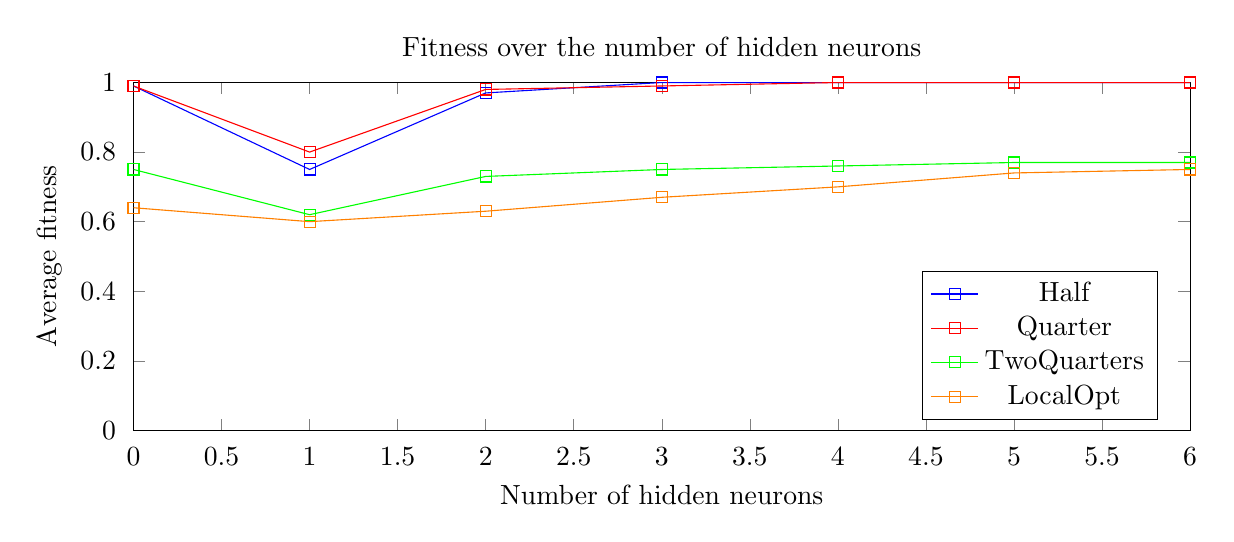
\begin{tikzpicture}
        \begin{axis}[
            width=15cm,
            height=6cm,
            legend pos=south east,
            title={Fitness over the number of hidden neurons},
            xlabel={Number of hidden neurons},
            ylabel={Average fitness},
            enlargelimits=false,
            xmin=0,
            ymin=0, ymax=1,
            ytick={0,0.2,...,1},
            xticklabel shift={.1cm},
            yticklabel shift={.1cm} ]
        ]

        \addplot[
            color=blue,
            mark=square,
            ]
            coordinates {
                (0,0.99)(1,0.75)(2,0.97)(3,1.00)(4,1.00)(5,1.00)(6,1.00)
            };
            \addlegendentry{Half}
        \addplot[
            color=red,
            mark=square,
            ]
            coordinates {
                (0,0.99)(1,0.80)(2,0.98)(3,0.99)(4,1.00)(5,1.00)(6,1.00)
            };
            \addlegendentry{Quarter}
        \addplot[
            color=green,
            mark=square,
            ]
            coordinates {
                (0,0.75)(1,0.62)(2,0.73)(3,0.75)(4,0.76)(5,0.77)(6,0.77)
            };
            \addlegendentry{TwoQuarters}
        \addplot[
            color=orange,
            mark=square,
            ]
            coordinates {
                (0,0.64)(1,0.60)(2,0.63)(3,0.67)(4,0.70)(5,0.74)(6,0.75)
            };
            \addlegendentry{LocalOpt}
        \end{axis}
        \end{tikzpicture}
        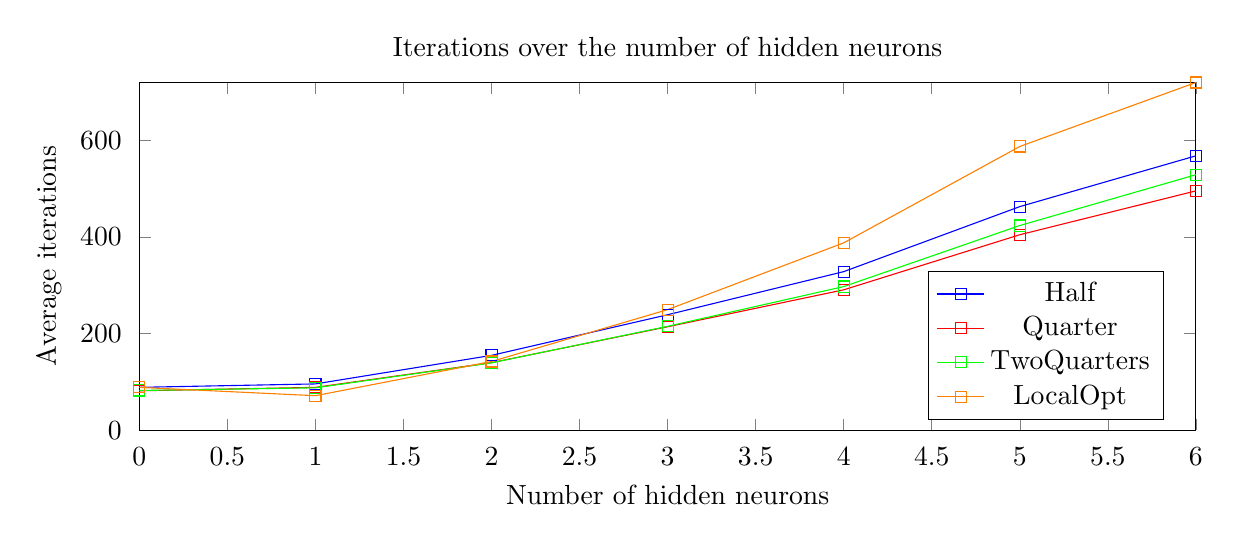
\begin{tikzpicture}
        \begin{axis}[
            width=15cm,
            height=6cm,
            legend pos=south east,
            title={Iterations over the number of hidden neurons},
            xlabel={Number of hidden neurons},
            ylabel={Average iterations},
            xmin=0,
            ymin=0,
            enlargelimits=false,
            xticklabel shift={.1cm},
            yticklabel shift={.1cm} ]
        ]

        \addplot[
            color=blue,
            mark=square,
            ]
            coordinates {
                (0,89.11)(1,96.17)(2,155.21)(3,239.27)(4,328.45)(5,462.97)(6,568.01)
            };
            \addlegendentry{Half}
        \addplot[
            color=red,
            mark=square,
            ]
            coordinates {
                (0,81.96)(1,89.09)(2,140.14)(3,214.40)(4,290.83)(5,404.78)(6,495.47)
            };
            \addlegendentry{Quarter}
        \addplot[
            color=green,
            mark=square,
            ]
            coordinates {
                (0,82.60)(1,88.10)(2,139.73)(3,215.31)(4,297.54)(5,423.82)(6,528.90)
            };
            \addlegendentry{TwoQuarters}
        \addplot[
            color=orange,
            mark=square,
            ]
            coordinates {
                (0,89.02)(1,71.80)(2,142.56)(3,249.84)(4,387.99)(5,587.37)(6,719.70)
            };
            \addlegendentry{LocalOpt}
        \end{axis}
        \end{tikzpicture}
        \begin{tikzpicture}
        \begin{axis}[
            width=15cm,
            height=6cm,
            legend pos=south east,
            title={CPU time over the number of hidden neurons},
            xlabel={Number of hidden neurons},
            ylabel={Average CPU time (s)},
            xmin=0,
            ymin=0,
            enlargelimits=false,
            xticklabel shift={.1cm},
            yticklabel shift={.1cm} ]
        ]

        \addplot[
            color=blue,
            mark=square,
            ]
            coordinates {
                (0,2.40)(1,3.18)(2,6.83)(3,12.22)(4,24.36)(5,36.22)(6,50.96)
            };
            \addlegendentry{Half}
        \addplot[
            color=red,
            mark=square,
            ]
            coordinates {
                (0,2.25)(1,2.79)(2,6.13)(3,9.47)(4,22.36)(5,32.22)(6,43.57)
            };
            \addlegendentry{Quarter}
        \addplot[
            color=green,
            mark=square,
            ]
            coordinates {
                (0,2.25)(1,2.91)(2,5.52)(3,9.99)(4,22.66)(5,32.81)(6,47.98)
            };
            \addlegendentry{TwoQuarters}
        \addplot[
            color=orange,
            mark=square,
            ]
            coordinates {
                (0,2.46)(1,2.32)(2,6.15)(3,12.54)(4,28.56)(5,46.02)(6,68.19)
            };
            \addlegendentry{LocalOpt}
        \end{axis}
        \end{tikzpicture}
    \end{center}
    \caption{Performance metrics of the CMA-ES algorithm on the unit-sphere classification benchmarks, over different number of hidden neurons.}
    \label{fig:cmaes_sphere}
\end{figure}

\subsubsection{Proben1 classification problems}

Finally, the CMA-ES algorithm was tested on the \textit{Proben1 Cancer1} problem, with fully connected networks with $0$ to $3$ hidden neurons. The results are presented in \Cref{fig:cmaes_proben1}.
Here, it was able to average a fitness of $0.98$, on the test set, for the $0, 2$ and $3$ hidden neurons cases, and $0.78$ for the $1$ hidden neuron case.
The number of iterations and CPU time increased with the number of hidden neurons, with the CPU time reaching $20.79$ seconds for $3$ hidden neurons, with $319$ iterations.

\begin{figure}
    \begin{center}
        \begin{tikzpicture}
        \begin{axis}[
            width=15cm,
            height=6cm,
            title={Fitness over the number of hidden neurons},
            xlabel={Number of hidden neurons},
            ylabel={Average fitness},
            enlargelimits=false,
            xmin=0,
            ymin=0, ymax=1,
            ytick={0,0.2,...,1},
            xticklabel shift={.1cm},
            yticklabel shift={.1cm} ]
        ]

        \addplot[
            color=blue,
            mark=square,
            ]
            coordinates {
                (0,0.98)(1,0.78)(2,0.96)(3,0.98)
            };
        \end{axis}
        \end{tikzpicture}
        \begin{tikzpicture}
        \begin{axis}[
            width=15cm,
            height=6cm,
            legend pos=south east,
            title={Iterations over the number of hidden neurons},
            xlabel={Number of hidden neurons},
            ylabel={Average iterations},
            xmin=0,
            ymin=0,
            enlargelimits=false,
            xticklabel shift={.1cm},
            yticklabel shift={.1cm} ]
        ]

        \addplot[
            color=blue,
            mark=square,
            ]
            coordinates {
                (0,148.35)(1,154.35)(2,223.47)(3,319.86)
            };
        \end{axis}
        \end{tikzpicture}
        \begin{tikzpicture}
        \begin{axis}[
            width=15cm,
            height=6cm,
            legend pos=south east,
            title={CPU time over the number of hidden neurons},
            xlabel={Number of hidden neurons},
            ylabel={Average CPU time (s)},
            xmin=0,
            ymin=0,
            enlargelimits=false,
            xticklabel shift={.1cm},
            yticklabel shift={.1cm} ]
        ]

        \addplot[
            color=blue,
            mark=square,
            ]
            coordinates {
                (0,5.99)(1,7.64)(2,12.99)(3,20.79)
            };
        \end{axis}
        \end{tikzpicture}
    \end{center}
    \caption{Performance metrics of the CMA-ES algorithm on the \textit{Proben1} benchmark, over different number of hidden neurons.}
    \label{fig:cmaes_proben1}
\end{figure}

\section{Discussion}

This section presents a comparison of the performance of the algorithms on the different benchmarks.
Then, based on this comparison, and the insights from the various experiments conducted and analyzed in \Cref{sec:results}, guidelines are proposed for the selection of the algorithm
based on the problem at hand, and for the selection of the parameters for the algorithms.

The comparison is based on the fitness and CPU time metrics, as the number of iterations/generations is not directly comparable between the different algorithms.
Furthermore, for each of the algorithm, the most efficient configuration were used to represent it in the comparison, where the efficiency is defined as a trade-off between the fitness
and the CPU time, with preference given to the fitness.

\subsection{Unit-sphere classification problems}

The performance of the algorithms on the unit-sphere classification problems is presented in \Cref{tab:comparison_sphere}.
All of the algorithms were able to solve the \textit{Half} and \textit{Quarter} problems.  However, the CPU time varied significantly between the algorithms, the $1 + 1$ NA and BNA algorithms
both required around $0.4$ seconds, while the NEAT algorithm required $127$ seconds.

For the \textit{TwoQuarters} problem, the $(1 + !)$ NA algorithm got the best fitness, followed by the BNA algorithm, while the NEAT and CMA-ES algorithms got values around $0.75$,
corresponding to the fitness value of a local-optima solution. However, the CMA-ES algorithm stopped after $6$ seconds compared to the $935$ seconds for the NEAT algorithm.
The same patterns were observed for the \textit{LocalOpt} problem.

Therefore, for these problems, the $(1 + 1)$ NA and BNA algorithm are the most efficient, with the NEAT algorithm being particularly slow and the CMA-ES algorithm unable to find the
optimal solutions to the problems.

\begin{table}[]
\caption{Comparison of the performance of the algorithms on the unit-sphere classification problems.}
\label{tab:comparison_sphere}
\centering
\begin{tabular}{|c|cccccccc|}
\hline
                   & \multicolumn{8}{c|}{\textbf{Problem}}                                                                                                                                                                                         \\ \hline
\textbf{}          & \multicolumn{2}{c|}{\textit{\textbf{Half}}}             & \multicolumn{2}{c|}{\textit{\textbf{Quarter}}}          & \multicolumn{2}{c|}{\textit{\textbf{TwoQuarters}}}      & \multicolumn{2}{c|}{\textit{\textbf{LocalOpt}}} \\ \hline
\textbf{Algorithm} & \multicolumn{1}{c|}{Fitness} & \multicolumn{1}{c|}{CPU} & \multicolumn{1}{c|}{Fitness} & \multicolumn{1}{c|}{CPU} & \multicolumn{1}{c|}{Fitness} & \multicolumn{1}{c|}{CPU} & \multicolumn{1}{c|}{Fitness}       & CPU        \\ \hline
\textbf{(1 +1) NA} & \multicolumn{1}{c|}{1.0}     & \multicolumn{1}{c|}{0.4} & \multicolumn{1}{c|}{1.0}     & \multicolumn{1}{c|}{0.4} & \multicolumn{1}{c|}{0.94}    & \multicolumn{1}{c|}{14}  & \multicolumn{1}{c|}{0.85}          & 15         \\ \hline
\textbf{BNA}       & \multicolumn{1}{c|}{1.0}     & \multicolumn{1}{c|}{0.4} & \multicolumn{1}{c|}{1.0}     & \multicolumn{1}{c|}{0.4} & \multicolumn{1}{c|}{0.85}    & \multicolumn{1}{c|}{14}  & \multicolumn{1}{c|}{0.80}          & 28         \\ \hline
\textbf{NEAT}      & \multicolumn{1}{c|}{1.0}     & \multicolumn{1}{c|}{127} & \multicolumn{1}{c|}{1.0}     & \multicolumn{1}{c|}{39}  & \multicolumn{1}{c|}{0.74}    & \multicolumn{1}{c|}{935} & \multicolumn{1}{c|}{0.65}          & 1134       \\ \hline
\textbf{CMA-ES}    & \multicolumn{1}{c|}{1.0}     & \multicolumn{1}{c|}{6}   & \multicolumn{1}{c|}{1.0}     & \multicolumn{1}{c|}{6}   & \multicolumn{1}{c|}{0.77}    & \multicolumn{1}{c|}{6}   & \multicolumn{1}{c|}{0.75}          & 68         \\ \hline
\end{tabular}
\end{table}

\subsection{XOR problem}

The performance of the algorithms on the \textit{XOR} problem is presented in \Cref{tab:comparison_xor}.
The NEAT algorithm achieved the best fitness, with $0.96$, followed by the CMA-ES algorithm with $00.93$. However, for this problem NEAT was also significantly slower than the other algorithms,
with a CPU time of $67$s, compared to $0.09$s for the CMA-ES algorithm and $0.01$ for the $(1 + 1)$ NA and BNA algorithms.
In addition, it can be noted how the fitness results are inverted compared to the unit-sphere classification problems, with the BNA and $(1 + 1)$ NA finding optimal solutions less often
than the NEAT and CMA-ES algorithms.
Thus, for this problem, the CMA-ES algorithm is the best choice, being comparable in speed to the $(1 + 1)$ NA and BNA algorithms, and in fitness to the NEAT algorithm.

\begin{table}
    \caption{Comparison of the performance of the algorithms on the \textit{XOR} benchmark.}
    \label{tab:comparison_xor}
    \centering
    \begin{tabular}{ |c|c|c| }
        \hline
        Algoeithm & Fitness & CPU time (s) \\
        \hline
        (1 + 1) NA & 0.83 & 0.01 \\
        \hline
        BNA & 0.79 & 0.01 \\
        \hline
        NEAT & 0.96 & 67 \\
        \hline
        CMA-ES & 0.93 & 0.09 \\
        \hline\hline
    \end{tabular}
\end{table}

\subsection{Proben1 classification problems}

The performance of the algorithms on the \textit{Proben1 Cancer1} problem is presented in \Cref{tab:comparison_proben1}.
The four algorithms reached high fitness values on the task. The CMA-ES algorithm needed the least CPU time, with $21$ seconds, followed by the NEAT algorithm with $37$ seconds.
For this problem, the $(1 + 1)$ NA and BNA algorithms were the slowest, with the BNA algorithm being almost three times slower than the $(1 + 1)$ NA algorithm.
Thus, the CMA-ES algorithm is the best choices for this problem, being the fastest, and reaching the same fitness as the NEAT algorithm.

\begin{table}
    \caption{Comparison of the performance of the algorithms on the \textit{Proben1 Cancer1} benchmark.}
    \label{tab:comparison_proben1}
    \centering
    \begin{tabular}{ |c|c|c| }
        \hline
        Algoeithm & Fitness & CPU time (s) \\
        \hline
        (1 + 1) NA & 0.96 & 72 \\
        \hline
        BNA & 0.96 & 199 \\
        \hline
        NEAT & 0.98 & 37 \\
        \hline
        CMA-ES & 0.98 & 21 \\
        \hline\hline
    \end{tabular}
\end{table}

\subsection{Double pole balancing problem}

The performance of the NEAT and CMA-ES algorithms on the double pole balancing problem is presented in \Cref{tab:comparison_pole}.
For this task, the NEAT algorithm is clearly the best choice, with a fitness of $1.0$, compared to $0.89$ for the CMA-ES algorithm, and a significantly lower CPU time, of $6.4$
seconds compared to $300$ seconds for the CMA-ES algorithm.

\begin{table}
    \caption{Comparison of the performance of the algorithms on the \textit{Double Pole Balancing} benchmark.}
    \label{tab:comparison_pole}
    \centering
    \begin{tabular}{ |c|c|c| }
        \hline
        Algoeithm & Fitness & CPU time (s) \\
        \hline
        NEAT & 1.0 & 6.4 \\
        \hline
        CMA-ES & 0.89 & 300 \\
        \hline\hline
    \end{tabular}
\end{table}

\subsection{Guidelines}

...
